% Gelfand seminar notes, 1972-73: source pages P000449-P000500.
% Russian diplomatic transcription (AI-made, checked against the scans), cut page by page from the cumulative working reader A4-reader-chapters01-29-first1358-separated-diplomatic-r2.
% \SourcePage{GELFAND-Pnnnnnn}{label} starts a scanned page; the second argument is the number written
% on the page, if any. Editorial notes give the page, a label and the transcriber's remark; \Unclear
% marks a doubtful reading.
\SourcePage{GELFAND-P000449}{71}
\SourceFigure{GELFAND-P000449}{quotient-conclusion}{Короткая косая черта соединяет $S$ с подписью.
\par\smallskip\centering\color{black}
\begingroup\color{black}\GelfandFitDiagram{\begin{tikzpicture}[x=1mm,y=1mm,every node/.style={inner sep=0pt}]
\node[anchor=base west] (exists) at (0,13) {$\exists$};
\node[anchor=base west] (subgroup) at ([xshift=1.5mm]exists.base east) {$S$};
\node[anchor=base west] at (subgroup.base east) {$\subset G$};
\node[anchor=base west] at (38,12.6) {$X\cong G/S$};
\draw ([xshift=.25mm,yshift=-1mm]subgroup.south)--++(1.15,-1.65);
\node[anchor=base west] at (12,8.2) {подгр.};
\node[anchor=base west] at (9,2.5) {(стабилиз.)};
\end{tikzpicture}}\endgroup}
\end{GelfandAdjacentEvidence}
\begin{GelfandAdjacentEvidence}{GELFAND-P000449}{2}


\SourceFigure{GELFAND-P000449}{closing-dots}{Десять точек образуют разделитель.
\par\smallskip\centering\color{black}
\begingroup\color{black}\GelfandFitDiagram{\begin{tikzpicture}[x=1mm,y=1mm]
\foreach \x/\y in {0/0,4/.3,9/.3,15/.4,22/.6,28/.6,33/.7,37/.5,41/.6,45/.4}
  \fill (\x,\y) circle [radius=.37mm];
\end{tikzpicture}}\endgroup}
\end{GelfandAdjacentEvidence}



\Needspace{7\baselineskip}
\begin{GelfandAdjacentEvidence}{GELFAND-P000450}{1}
\SourcePage{GELFAND-P000450}{unlabelled}
\uuline{\mbox{$25/\underline{\overline{\mathrm{IX}}}$}-72\,г.}
\quad\uuline{Габриэлов.}

Сем-во структур Ходжа над $S$ (неособое аналит. мн-зие)
\Unclear{GELFAND-P000450}{non-singular-word}{После «б» два соединённых округлых штриха. Набрано «неособое».}
\end{GelfandAdjacentEvidence}
\begin{GelfandAdjacentEvidence}{GELFAND-P000450}{2}


$1)$ $\mathcal H_{\mathbb Z}$ — лок. своб. пучок $\mathbb Z$-модулей конечн. типа.

\sout{2)}\quad По нему стр. лок. трив. компл. рассл. $H_{\mathbb C}$.
\Unclear{GELFAND-P000450}{cancelled-number}{Зачёркнутое начало строки предположительно «2)».}
\end{GelfandAdjacentEvidence}
\begin{GelfandAdjacentEvidence}{GELFAND-P000450}{3}


\SourceFigure{GELFAND-P000450}{deligne-annotation}{Стрелка от записи комплексного продолжения направлена к заметке. Нижняя черта заметки загнута слева вверх.
\par\smallskip\centering\color{black}
\begingroup\color{black}\GelfandFitDiagram{\begin{tikzpicture}[x=1mm,y=1mm,every node/.style={font=\scriptsize,inner sep=0pt,anchor=base west}]
\node (complex) at (0,16)
  {$H_{\mathbb C}=H_{\mathbb Z}\otimes_{\mathbb Z}\mathbb C,$};
\node at ([xshift=3mm]complex.base east)
  {$H_{\mathcal O}=H_{\mathbb Z}\otimes_{\mathbb Z}\mathcal O_S$.};
\node at (0,8) {и $H_{\mathbb R}$ — вещ. расслоение.};
\node (localsystem) at (36,8) {лок. система (Делинь) —};
\node (bundle) at (40,3.4) {— рассл. со связностью.};
\draw[->] ([xshift=-1mm,yshift=-.8mm]complex.south east)
  -- ([xshift=-1mm,yshift=.25mm]localsystem.base west);
\draw (33,7.8) .. controls (32,2) and (34.4,1.6) .. (37,1.2)
  -- ([xshift=2mm,yshift=-1mm]bundle.south east);
\end{tikzpicture}}\endgroup}
\end{GelfandAdjacentEvidence}
\begin{GelfandAdjacentEvidence}{GELFAND-P000450}{4}


$2)$ в $H_{\mathbb C}$ убывающая фильтрация голом. расслоениями
\[
H_{\mathbb C}=F^0\supset F^1\supset\ldots\supset F^n
\]

\SourceFigure{GELFAND-P000450}{connection-bubble}{Вписанное «есть» охвачено петлёй.
\par\smallskip\centering\color{black}
\begingroup\color{black}\GelfandFitDiagram{\begin{tikzpicture}[x=1mm,y=1mm,every node/.style={font=\scriptsize,inner sep=0pt,anchor=base west}]
\node (prefix) at (0,4) {$3)$ в $H_{\mathcal O}$};
\node (natural) at ([xshift=4mm]prefix.base east) {естеств. связность (Гаусса—Манина)};
\node (exists) at ([xshift=-.7mm,yshift=5.8mm]natural.base west) {есть};
\coordinate (tail) at ([xshift=-2mm,yshift=.4mm]natural.base west);
\draw ([xshift=-2mm,yshift=.5mm]exists.north west)
  .. controls ([xshift=2mm,yshift=3mm]exists.north west) and
              ([xshift=2mm,yshift=2.6mm]exists.north east) ..
              ([xshift=1.5mm,yshift=.55mm]exists.north east)
  .. controls ([xshift=3mm,yshift=-1mm]exists.north east) and
              ([xshift=3.1mm,yshift=-.8mm]exists.south east) ..
              ([xshift=1.2mm,yshift=-1.2mm]exists.south east)
  .. controls ([xshift=2mm,yshift=-1.5mm]exists.south west) and
              ([xshift=-.8mm,yshift=-1.6mm]exists.south west) .. (tail)
  .. controls ([xshift=-2mm,yshift=-.6mm]exists.south west) and
              ([xshift=-1.6mm,yshift=.5mm]exists.south west) ..
              ([xshift=-1.55mm,yshift=.5mm]exists.north west);
\end{tikzpicture}}\endgroup}
\end{GelfandAdjacentEvidence}
\begin{GelfandAdjacentEvidence}{GELFAND-P000450}{5}

\Unclear{GELFAND-P000450}{connection-name}{Серединные буквы первой фамилии соединены. Набрано «Гаусса—Манина».}
\end{GelfandAdjacentEvidence}
\begin{GelfandAdjacentEvidence}{GELFAND-P000450}{6}


\SourceFigure{GELFAND-P000450}{kernel-caption}{Заметка о ядре стоит справа от формулы. Знак перед тире предположительно запятая.
\par\smallskip\centering\color{black}\scriptsize
\begin{tabular}{@{}p{.53\linewidth}@{\enspace}p{.42\linewidth}@{}}
$\nabla\colon H_{\mathcal O}\longrightarrow\Omega^1\otimes_{\mathcal O_S}H_{\mathcal O}$
& \raggedright (дифф. опер. с ядром, — сеч. $H_{\mathbb C}$).\tabularnewline
\end{tabular}}
\end{GelfandAdjacentEvidence}
\begin{GelfandAdjacentEvidence}{GELFAND-P000450}{7}


(есть лок. пост. сечения $\mathbb Z$ — образ пучка $H_{\mathbb C}$)
\Unclear{GELFAND-P000450}{local-section-glyph}{Знак между «сечения» и тире предположительно $\mathbb Z$. У него петля и длинный нижний штрих. Точное чтение не установлено.}
\end{GelfandAdjacentEvidence}
\begin{GelfandAdjacentEvidence}{GELFAND-P000450}{8}


Связность должна удовл. условию:
\[
\nabla(\mathcal F^p)\subset\Omega_S^1\otimes\mathcal F^{p-1}
\qquad(\mathcal F^p=F^p\otimes_{\mathbb C}\mathcal O_S)
\]

$4)$ $\psi$ — билин., лок. пост. форма на $H_{\mathbb C}$, дающая при огранич. на $\forall$ слой настоящую структ. Ходжа.

\begin{center}
\rule[.5ex]{16mm}{.35pt}\enspace$\bullet$\enspace\rule[.5ex]{19mm}{.35pt}
\end{center}
Классифицир. пр-во структур Ходжа.

Рассм.\par
\hfill\rule[.5ex]{15mm}{.35pt}\enspace$\bullet$\enspace\rule[.5ex]{15mm}{.35pt}\hspace{20mm}
\[
F=\{F^0\supset F^1\supset\ldots\supset F^n\}
\qquad\text{— флаги }\mbox{\uuline{фиксир.}\ \uuline{разм.}}
\]

в фикс. пр-ве, $\mathbb C^n$ ($\dim$ могут быть с пропусками).
\begin{center}
\rule[.5ex]{16mm}{.35pt}\enspace$\bullet$\enspace\rule[.5ex]{16mm}{.35pt}
\end{center}
\SourceFigure{GELFAND-P000450}{flag-margin}{Две вертикальные черты отделяют запись на правом поле.
\par\smallskip\hfill\color{black}
\begin{tabular}{@{}||@{\enspace}l@{}}
набор $\dim$ —\\
— задаётся.
\end{tabular}}
\end{GelfandAdjacentEvidence}
\begin{GelfandAdjacentEvidence}{GELFAND-P000450}{9}


\underline{$D$} — пр-во;

Точки пр-ва \sout{\mbox{$D$}} — \underline{флаги}.
\Unclear{GELFAND-P000450}{point-cancel}{Густо наведённый знак перед тире напоминает $D$. Чтение зачёркнутой буквы предположительно.}
\end{GelfandAdjacentEvidence}
\begin{GelfandAdjacentEvidence}{GELFAND-P000450}{10}


Берём лин. пр-во \uuline{\mbox{$H_{\mathbb C}$}} с билин. формой $\psi(x,y)$
(невырожд.; кос. либо симм.)
\SourceFigure{GELFAND-P000450}{space-underlines}{Две черты под $H_{\mathbb C}$ проходят ниже опущенного индекса.}
\end{GelfandAdjacentEvidence}
\begin{GelfandAdjacentEvidence}{GELFAND-P000450}{11}


$\bar D$ — мн-зие всех флагов \sout{в} в $H_{\mathbb C}$
с фикс. набором $\dim$
\Unclear{GELFAND-P000450}{bar-d}{Над жирно наведённой $D$ видна отдельная черта.}
\end{GelfandAdjacentEvidence}
\begin{GelfandAdjacentEvidence}{GELFAND-P000450}{12}

\Unclear{GELFAND-P000450}{bottom-cancellation}{Малый зачёркнутый знак перед «в» набран предположительно как ещё одно «в».}
\end{GelfandAdjacentEvidence}



\Needspace{7\baselineskip}
\begin{GelfandAdjacentEvidence}{GELFAND-P000451}{1}
\SourcePage{GELFAND-P000451}{72}
\sout{\ldots}\quad с условием $1)$ $\psi(F^p,F^{n-p})=0$.
\Incomplete{GELFAND-P000451}{initial-cancel}{Короткий зачёркнутый знак перед «с» не разобран.}
\end{GelfandAdjacentEvidence}
\begin{GelfandAdjacentEvidence}{GELFAND-P000451}{2}

\Unclear{GELFAND-P000451}{orthogonality-exponent}{В первой формуле отчётливо написано $n-p$. В следующей формуле отдельно написано $n-p+1$.}
\end{GelfandAdjacentEvidence}
\begin{GelfandAdjacentEvidence}{GELFAND-P000451}{3}


Это алгебраич. подмн-зие $\bar D$.

$\psi$ либо симм., либо кососимметрич. \uuline{(def)}.

\[
2)\quad F^p\oplus\bar F^{n-p+1}\cong H_{\mathbb C}
\]
\Unclear{GELFAND-P000451}{complement-sign}{Знак перед $H_{\mathbb C}$ имеет волну над двумя горизонтальными чертами. Нижние черты соединены косым штрихом. Набрано предположительно $\cong$. Начертание $H$ густо наведено.}
\end{GelfandAdjacentEvidence}
\begin{GelfandAdjacentEvidence}{GELFAND-P000451}{4}

\[
H_{\mathbb Z}\subset H_{\mathbb R}\subset H_{\mathbb C}
\qquad\mbox{\uuline{тоже задано}}
\]

По невыр. флагу опр. градуировка и автом. Вейля
\[
H^{p,n-p}=F^p\cap\bar F^{n-p}
\]
Автом. Вейля:
\[
C\xi=i^{2p-n}\xi\quad\text{при }\xi\in H^{p,n-p}
\]
Эти усл. выделяют в $\bar D$ откр. подмн-зие $D$.

\sout{\ldots}\qquad Ещё условие:\quad $\psi(x,C\bar x)>0$ при $x\ne0$.
\Incomplete{GELFAND-P000451}{condition-cancel}{Перед «Ещё условие» несколько горизонтальных штрихов перекрывают прежнюю запись. Виден конец с петлёй и точкой. Текст не восстановлен.}
\end{GelfandAdjacentEvidence}
\begin{GelfandAdjacentEvidence}{GELFAND-P000451}{5}


Определим на $D$ структуру однор. пр-ва.

$G$ — группа всех вещ. преобр. $H_{\mathbb R}$, сохр. $\psi$
\[
\bigl(\psi(gx,gy)=\psi(x,y)\bigr).
\]
\Unclear{GELFAND-P000451}{group-equation}{Левая внешняя скобка густо наведена. Справа различимы две круглые скобки.}
\end{GelfandAdjacentEvidence}
\begin{GelfandAdjacentEvidence}{GELFAND-P000451}{6}


\uwave{Тогда \mbox{$G$} действует на \mbox{$D$}}

\SourceFigure{GELFAND-P000451}{theorem-insert}{Перед $G$ видна отдельная запись, предположительно «яв.», и густо наведённый знак. В петлю над ним вписано $1$. У начала строки предположительно $1)$.
\par\smallskip\centering\color{black}
\begingroup\color{black}\GelfandFitDiagram{\begin{tikzpicture}[x=1mm,y=1mm,every node/.style={anchor=base west,inner sep=0pt,font=\scriptsize}]
\node (theorem) at (0,4) {\underline{Теорема}:};
\node (old) at ([xshift=1mm]theorem.base east) {$1)$ яв. \sout{\ldots}};
\node (g) at ([xshift=1.2mm]old.base east) {$G$ действ. транзитивно};
\node at ([xshift=-1.7mm,yshift=5.7mm]g.base west) {$1$};
\coordinate (tail) at ([xshift=-.7mm,yshift=.4mm]g.base west);
\draw ([xshift=-3.35mm,yshift=7.1mm]g.base west)
  .. controls ([xshift=-1.95mm,yshift=5.6mm]g.base west) and
              ([xshift=-1.15mm,yshift=3.3mm]g.base west) .. (tail)
  .. controls ([xshift=-.05mm,yshift=3.15mm]g.base west) and
              ([xshift=1.6mm,yshift=5.45mm]g.base west) ..
              ([xshift=1.55mm,yshift=7.05mm]g.base west)
  .. controls ([xshift=1.35mm,yshift=8.75mm]g.base west) and
              ([xshift=-.25mm,yshift=9.5mm]g.base west) ..
              ([xshift=-2.35mm,yshift=8.55mm]g.base west);
\end{tikzpicture}}\endgroup}
\end{GelfandAdjacentEvidence}


$2)$ ст. Подгруппа $H$ (сохр. флаг.) компактна.

\underline{Док-во:}\quad из явного вычисления $G$ и $H$.

$K\subset G$ — макс. комп. подгруппа

$G/H\longrightarrow G/K$\quad оно не голоморфно

В $G/K$ есть компл. структура


\Needspace{7\baselineskip}
\begin{GelfandAdjacentEvidence}{GELFAND-P000452}{1}
\SourcePage{GELFAND-P000452}{unlabelled}
\underline{\sout{\ldots}}.\qquad
\rule[.5ex]{13mm}{.35pt}\enspace$\cdot$\enspace\rule[.5ex]{17mm}{.35pt}
\Incomplete{GELFAND-P000452}{title-cancel}{Подчёркнутый заголовок закрыт частыми волнистыми штрихами. Видна точка справа. Буквы не восстановлены.}
\end{GelfandAdjacentEvidence}
\begin{GelfandAdjacentEvidence}{GELFAND-P000452}{2}


\underline{1-я лекция Манина о \mbox{$p$}-адич. числах.}\quad (пересказ)

$K$ — лок. поле, (\sout{\ldots}
\Incomplete{GELFAND-P000452}{k-cancel}{После запятой видна левая скобка и густо зачёркнутая короткая запись. Правая скобка в этой строке не различается.}
\end{GelfandAdjacentEvidence}
\begin{GelfandAdjacentEvidence}{GELFAND-P000452}{3}

(кон. расш. $p$-адич. числах)\quad
\sout{или форм. степ. ряды над}\par\hspace{23mm}\sout{кон. полем})
\Incomplete{GELFAND-P000452}{parent-cancel-full}{Под зачёркиванием предположительно «или форм. степ. ряды над» и строкой ниже «кон. полем». Возле слов «адич. чисел» закрывающая скобка сильно наведена.}
\end{GelfandAdjacentEvidence}
\begin{GelfandAdjacentEvidence}{GELFAND-P000452}{4}


\SourceFigure{GELFAND-P000452}{maximal-ideal-annotation}{Короткая вертикальная черта соединяет $m$ с подписью ниже.
\par\smallskip\centering\color{black}
\begingroup\color{black}\GelfandFitDiagram{\begin{tikzpicture}[x=1mm,y=1mm,every node/.style={anchor=base west,inner sep=0pt}]
\node (ring) at (0,9) {$A$ — кольцо целых,};
\node (ideal) at ([xshift=3mm]ring.base east) {$m$};
\node at (ideal.base east) {$\subset A$};
\draw ([xshift=-.15mm,yshift=-.4mm]ideal.south) -- ++(-.18,-2.1);
\node at ([xshift=-2.7mm,yshift=-6.8mm]ideal.base west) {макс. идеал};
\end{tikzpicture}}\endgroup}
\end{GelfandAdjacentEvidence}
\begin{GelfandAdjacentEvidence}{GELFAND-P000452}{5}


$P^1(K)$ — проект. прямая.
\[
\begin{aligned}
G &= \text{дв-ния её}\quad
   \left\{z\longrightarrow\frac{az+b}{cz+d}\ \middle|\ 
     a,b,c,d\in K,\ \det\ne0\right\}=\\
  &= \operatorname{GL}(2,K)/K^*
\end{aligned}
\]
\Unclear{GELFAND-P000452}{mobius-det}{Перед правой фигурной скобкой написано $\det\ne0$. Знак густо наведён. Два горизонтальных штриха сразу справа от скобки читаются как $=$. Следующая строка тоже начинается с $=$.}
\end{GelfandAdjacentEvidence}
\begin{GelfandAdjacentEvidence}{GELFAND-P000452}{6}


$U\subset G$;\quad $U=\operatorname{GL}(2,A)/A^*$.

Постр. $G/U$ — граф $\Delta$ — аналог плоск. Лобачевского.

\underline{Опр.}: решётка в $K^2$ — своб. $A$-модуль с 2-мя образ.
\[
L=Ae_1\oplus Ae_2.
\]
\underline{Лемма}. Если $L_1$ и $L_2$ — 2 реш.,
то $\exists$ базис $e_1,e_2$ в $K^2$, такой, что
\[
\begin{gathered}
L_1=Ae_1\oplus Ae_2;\qquad L_2=m^{\nu_1}e_1\oplus m^{\nu_2}e_2=\\
{}=A\pi^{\nu_1}e_1\oplus A\pi^{\nu_2}e_2
\end{gathered}
\]

\hfill($\pi$ — образующая [?] макс. идеала)
\Unclear{GELFAND-P000452}{ideal-symbol-tight}{Между «образующая» и «макс.» виден петлеобразный знак с продольным штрихом. Чтение не установлено.}
\end{GelfandAdjacentEvidence}
\begin{GelfandAdjacentEvidence}{GELFAND-P000452}{7}


\SourceFigure{GELFAND-P000452}{integer-note}{Запись $\nu_1,\nu_2\in\mathbb Z$ стоит справа между строками двух скобок.
\par\smallskip\color{black}
(аналог. теор. лин. алг. об одновр. приведении)\hfill
\raisebox{1ex}{$\nu_1,\nu_2\in\mathbb Z$}}
\end{GelfandAdjacentEvidence}
\begin{GelfandAdjacentEvidence}{GELFAND-P000452}{8}


\underline{Def.}\quad $L_1\sim L_2$, если
\underline{$L_1=\alpha L_2$}, где $\alpha\in K^*$.

\begin{center}
\rule[.5ex]{17mm}{.35pt}\enspace$\cdot$\enspace\rule[.5ex]{19mm}{.35pt}
\end{center}
Есть аналог расстояния — как в симм. пр-вах. \sout{\ldots}\ — см. \underline{А. Вейль}
\Incomplete{GELFAND-P000452}{sim-margin-cancel}{Малый знак перед тире перечёркнут. Чтение не установлено.}
\end{GelfandAdjacentEvidence}
\begin{GelfandAdjacentEvidence}{GELFAND-P000452}{9}


\begin{center}
\rule[.5ex]{17mm}{.35pt}\enspace$\cdot$\enspace\rule[.5ex]{19mm}{.35pt}
\end{center}
Вершины графа $\Delta^{(0)}_{\text{\sout{\ldots}}}$ — классы экв. решёток
\Incomplete{GELFAND-P000452}{dimension-glyph}{Справа внизу от первого $\Delta$ виден зачёркнутый малый знак. Его чтение не установлено. Над ним стоит $(0)$.}
\end{GelfandAdjacentEvidence}


$G$ действ. на $\Delta^{(0)}$.


\Needspace{7\baselineskip}
\begin{GelfandAdjacentEvidence}{GELFAND-P000453}{1}
\SourcePage{GELFAND-P000453}{73}
\SourceFigure{GELFAND-P000453}{class-arrow}{Стрелка при $\Delta^{(0)}$ направлена влево вниз к первой записи.
\par\smallskip\centering\color{black}
\begingroup\color{black}\GelfandFitDiagram{\begin{tikzpicture}[x=1mm,y=1mm,every node/.style={inner sep=0pt,anchor=base west,font=\scriptsize}]
\node (first) at (0,1) {$\Lambda_1=\{L_1\},$};
\node at ([xshift=2.5mm]first.base east) {$\Lambda_2=\{L_2\}$ — классы решёток.};
\node at (15,10.3) {$\Delta^{(0)}$};
\draw[->] (15.15,8.9) -- (12.55,5.7);
\end{tikzpicture}}\endgroup}
\end{GelfandAdjacentEvidence}
\begin{GelfandAdjacentEvidence}{GELFAND-P000453}{2}


\SourceFigure{GELFAND-P000453}{inclusion-and-residue}{Рамка под $L_2\subset L_1$ открыта сверху. Справа две вертикальные черты отделяют запись поля вычетов. У $F$ удвоен левый штрих.
\par\smallskip\centering\color{black}
\begingroup\color{black}\GelfandFitDiagram{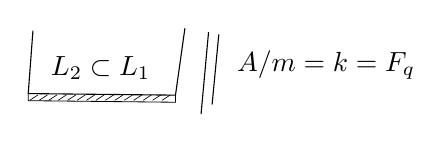
\begin{tikzpicture}[x=1mm,y=1mm]
\node[inner sep=0pt] at (11,7.8) {$L_2\subset L_1$};
\draw (2.4,12.6)--(1.8,4.6)--(20.5,4.4)--(21.7,12.9);
\draw[line width=.3pt] (1.8,4.6)--(1.8,3.7)--(20.5,3.5)--(20.5,4.4);
\foreach \x in {2.0,3.2,...,19.4}{\draw[line width=.24pt] (\x,3.75)--++(1.05,.68);}
\draw (24.7,12.4)--(23.75,2) (26,12.1)--(25.15,3.2);
\node[anchor=west,inner sep=0pt] at (28.25,8.2) {$A/m=k=\mathbb F_q$};
\end{tikzpicture}}\endgroup}
\end{GelfandAdjacentEvidence}
\begin{GelfandAdjacentEvidence}{GELFAND-P000453}{3}


\[
\begin{gathered}
L_1=Ae_1\oplus Ae_2\\
L_2=Ae_1\oplus A\pi^\nu e_2
\end{gathered}
\]
— так выбир. представители,\quad \uuline{\mbox{$\nu\ge0$}.}
\Unclear{GELFAND-P000453}{representative-word}{Окончание последнего слова бледное. Читается «представители».}
\end{GelfandAdjacentEvidence}
\begin{GelfandAdjacentEvidence}{GELFAND-P000453}{4}


$\nu$ наз. расстоянием\qquad \uuline{\mbox{$\nu=d(\Lambda_1,\Lambda_2)$}.}

\SourceFigure{GELFAND-P000453}{quotient-cancel}{Три черты охватывают формулу снизу и с боков. Запись после знака равенства густо зачёркнута. Её чтение не установлено.
\par\smallskip\centering\color{black}
\begingroup\color{black}\GelfandFitDiagram{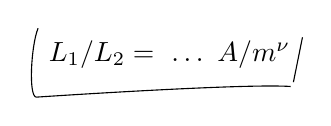
\begin{tikzpicture}[x=1mm,y=1mm]
\node[inner sep=0pt,anchor=base west] (quotient) at (3,5.1)
  {$L_1/L_2={}$ \sout{\ldots}\ $A/m^\nu$};
\path ([yshift=-2.25mm]quotient.south east) coordinate (right);
\draw (1.7,9.3) .. controls (.8,7.1) and (.45,.5) .. (1.5,.55)
  .. controls (9,1.05) and ([xshift=-5mm,yshift=.35mm]right) .. (right);
\draw ([xshift=.35mm,yshift=.55mm]right)--++(1.15,5.7);
\end{tikzpicture}}\endgroup}
\end{GelfandAdjacentEvidence}
\begin{GelfandAdjacentEvidence}{GELFAND-P000453}{5}


\underline{Теор.}\quad Это корр. опр. и есть \underline{расстояние}.
\begin{center}
\rule[.5ex]{14mm}{.35pt}\enspace$\cdot$\enspace\rule[.5ex]{21mm}{.35pt}
\end{center}

\uuline{Вариант:}
\[
L_1/L_2\simeq A/\pi^{\nu_1}A\oplus A/\pi^{\nu_2}A
\]
\Unclear{GELFAND-P000453}{variant-sign}{Одна прямая черта под волной. Набрано $\simeq$.}
\end{GelfandAdjacentEvidence}
\begin{GelfandAdjacentEvidence}{GELFAND-P000453}{6}

\[
d(\Lambda_1,\Lambda_2)=|\nu_1-\nu_2|
\]

$\Lambda_1,\Lambda_2$ — соседи в $\Lambda^0$, если $d(\Lambda',\Lambda^2)=1$.
\Unclear{GELFAND-P000453}{neighbor-notation}{В записи множества видны $\Lambda$ и малый верхний круг. В аргументах $d$ справа от первой $\Lambda$ стоит верхний штрих, справа от второй — верхняя $2$.}
\end{GelfandAdjacentEvidence}
\begin{GelfandAdjacentEvidence}{GELFAND-P000453}{7}


Соед. их ребром. Получим граф $\Delta$.

\underline{Теорема}:\quad $\Delta$ — дерево (св. граф без циклов),
причём из $\forall$ верш. вых. точно $q+1$ ребро

$\Delta$ и есть плоск. Лобач. — действует $G$ и т.д.

\SourceFigure{GELFAND-P000453}{disk-figure}{Внешняя граница имеет разрыв справа вверху. Внутренние дуги и цепочка воспроизведены по видимым штрихам. Тонкий знак у нижней левой дуги похож на овал. Некоторые соединения в верхней правой части остаются сомнительными.
\par\smallskip\centering\color{black}
\begingroup\color{black}\GelfandFitDiagram{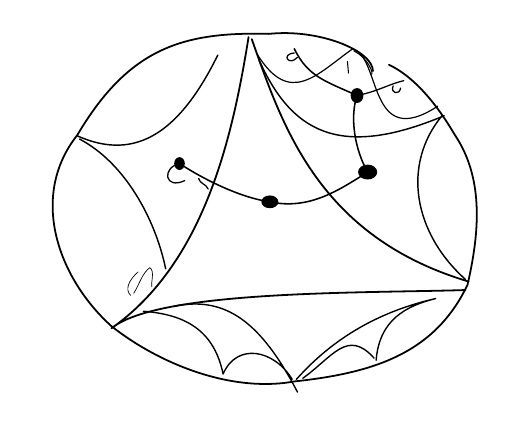
\begin{tikzpicture}[x=.135mm,y=-.135mm,line cap=round,line join=round]
% The outline is broken near the top right, as in the manuscript.
\draw[line width=.64pt] (325,52)
  .. controls (325,33) and (275,12) .. (227,17)
  .. controls (148,15) and (96,29) .. (47,112)
  .. controls (1,170) and (29,247) .. (79,292)
  .. controls (122,326) and (190,355) .. (251,344)
  .. controls (325,336) and (383,318) .. (414,253)
  .. controls (424,209) and (431,155) .. (402,112)
  .. controls (382,78) and (361,56) .. (340,46);
% Main arcs and boundary wedges.
\draw[line width=.65pt] (208,20) .. controls (193,113) and (167,232) .. (79,294)
  .. controls (123,258) and (314,261) .. (412,258);
\draw[line width=.65pt] (211,22) .. controls (240,104) and (274,208) .. (415,250);
\draw[line width=.52pt] (47,113) .. controls (103,138) and (144,108) .. (179,37)
  (49,116) .. controls (91,138) and (120,190) .. (130,238);
\draw[line width=.52pt] (218,42) .. controls (248,108) and (292,136) .. (392,94)
  (390,94) .. controls (352,140) and (363,204) .. (412,248);
\draw[line width=.43pt] (216,36) .. controls (247,86) and (272,55) .. (306,31)
  .. controls (333,39) and (320,128) .. (386,85);
\draw[line width=.37pt] (307,33) .. controls (320,39) and (327,56) .. (323,55)
  (301,43)--(302,54);
\draw[line width=.5pt] (109,278) .. controls (151,281) and (176,298) .. (184,337)
  .. controls (197,307) and (232,314) .. (249,342)
  (139,273) .. controls (186,264) and (219,287) .. (254,354)
  (253,342) .. controls (285,306) and (327,279) .. (384,266)
  .. controls (356,273) and (331,286) .. (328,324)
  (259,341) .. controls (287,321) and (301,294) .. (326,322);
% Inner chain, its short branches, and the separate fine lower-left mark.
\draw[line width=.56pt] (143,139) .. controls (166,154) and (200,171) .. (228,175)
  .. controls (265,183) and (293,164) .. (320,147)
  .. controls (308,126) and (303,96) .. (310,75)
  .. controls (282,62) and (264,58) .. (251,31);
\draw[line width=.46pt] (310,75) .. controls (330,71) and (338,65) .. (354,61)
  (143,139) .. controls (126,143) and (129,164) .. (148,155)
  (161,153) .. controls (162,158) and (168,158) .. (170,163)
  (251,35) .. controls (238,36) and (246,48) .. (254,39)
  (344,66) .. controls (341,73) and (350,75) .. (351,68);
\fill (143,139) ellipse [x radius=5,y radius=6];
\fill (228,175) ellipse [x radius=8,y radius=6];
\fill (320,147) ellipse [x radius=9,y radius=7];
\fill (310,75) ellipse [x radius=6,y radius=7];
\draw[line width=.25pt] (97,263) .. controls (91,257) and (96,248) .. (104,241)
  (100,261) .. controls (105,253) and (108,242) .. (115,237)
  .. controls (120,240) and (116,250) .. (117,255);
\end{tikzpicture}}\endgroup}
\end{GelfandAdjacentEvidence}


\begin{center}
\rule[.5ex]{18mm}{.35pt}\enspace$\bullet$\enspace\rule[.5ex]{21mm}{.35pt}
\end{center}


\Needspace{7\baselineskip}
\begin{GelfandAdjacentEvidence}{GELFAND-P000454}{1}
\SourcePage{GELFAND-P000454}{unlabelled}
\uuline{Д. Каждан}.\quad Ст. Тэйта, Математика, \underline{$13:2$, §$3$}.

(о поле $\mathbb C_p$ — пополнении алг. замык. $\overline{\mathbb Q}_p$ или
$\mathbb Q_p$ — $p$-адич. чисел)
\Unclear{GELFAND-P000454}{q-p-link-word}{Связующее слово читается «или».}
\end{GelfandAdjacentEvidence}
\begin{GelfandAdjacentEvidence}{GELFAND-P000454}{2}


\begin{center}
\rule[.5ex]{14mm}{.35pt}\enspace$\cdot$\enspace\rule[.5ex]{21mm}{.35pt}
\end{center}

$K$ — конечн. расш. поля $\mathbb Q_p$.

\SourceFigure{GELFAND-P000454}{vertical-ring}{Между двумя записями виден кривой штрих. Его значение не установлено. Под второй записью стоят два коротких вертикальных штриха.
\par\smallskip\centering\color{black}
\begingroup\color{black}\GelfandFitDiagram{\begin{tikzpicture}[x=1mm,y=1mm,line cap=round,every node/.style={inner sep=0pt,anchor=base west,font=\scriptsize}]
\node at (0,1) {$k=\mathcal O_K/m_K$.};
\node at (23,16.5) {$\mathcal O_K$ — целые в $K$.};
\draw (23.6,13.6) .. controls (23.2,12.55) and (23.45,11.3) .. (24.35,11.7)
  .. controls (25.15,12.05) and (25.95,13.2) .. (26.55,14.35);
\node at (23,7.7) {$m_K$ — макс. идеал};
\draw (24.65,5.25)--(24.55,4.35) (25.9,5.3)--(26.05,4.2);
\node at (23,1) {$(\pi)$.};
\end{tikzpicture}}\endgroup}
\end{GelfandAdjacentEvidence}
\begin{GelfandAdjacentEvidence}{GELFAND-P000454}{3}


$L$ — конечн. расш. $K$, \sout{\ldots} $\mathcal O_L$ — целые в нём

\Unclear{GELFAND-P000454}{ol-cancel}{Зачёркнутые штрихи перед $\mathcal O_L$ не разобраны.}
\end{GelfandAdjacentEvidence}
\begin{GelfandAdjacentEvidence}{GELFAND-P000454}{4}


$m_L=(\tau)$,\quad $\ell=\mathcal O_L/m_L$,
\[
G=\operatorname{Gal}(L:K)
\]
Введ. фильтрацию в $G$ и док., что $G$ разрешимо.

На $L$ и $K$ \sout{\ldots} зададим норму, так что
$|\pi|=(\operatorname{Card}k)^{-1}$
\Unclear{GELFAND-P000454}{norm-cancel}{Между $K$ и «зададим» виден зачёркнутый знак. Его чтение не установлено.}
\end{GelfandAdjacentEvidence}
\begin{GelfandAdjacentEvidence}{GELFAND-P000454}{5}


\uuline{Def.}\quad \sout{\ldots}.
\Incomplete{GELFAND-P000454}{def-cancel}{После «Def.» зачёркнута короткая запись. Её чтение не установлено.}

\[
g\in G_i\Longleftrightarrow \forall x\in \mathcal O_L\quad x^g-x\in m_L^i
\]
\[
G=G_0\supset G_1\supset\ldots\supset G_n=\{e\}.
\]
\end{GelfandAdjacentEvidence}
\begin{GelfandAdjacentEvidence}{GELFAND-P000454}{6}
$G_i$ — норм. делитель в $G$.

\underline{Теорема:}\quad $G_i/G_{i+1}$ — аб. группа

$1)$ \underline{$i=0$.}\qquad
$G\overset{\varphi}{\longrightarrow}\operatorname{Gal}(\ell:k)$
(естеств. отобр.)

\underline{Построение $\varphi$:}\quad $\bar x\in\ell,\ g\in G$
\[
x\in L\qquad \bar x^g\overset{\mathrm{def}}{=}\overline{x^g}
\]
\Unclear{GELFAND-P000454}{residue-representative}{В рукописи читается $x\in L$.}
\end{GelfandAdjacentEvidence}
\begin{GelfandAdjacentEvidence}{GELFAND-P000454}{7}


$g\in\ker\varphi\Longleftrightarrow \bar x\in\ell,\ \bar x^g=\bar x$,
т.е. $\bar x^g-\bar x=0$, т.е.
\Unclear{GELFAND-P000454}{kernel-quantifier}{После знака равносильности читается $\bar x\in\ell$. Явный квантор не виден.}
\end{GelfandAdjacentEvidence}



\Needspace{7\baselineskip}
\begin{GelfandAdjacentEvidence}{GELFAND-P000455}{1}
\SourcePage{GELFAND-P000455}{74}
\sout{т.е. \ldots}\qquad $x^g-x\in m_L$, т.е. $g\in G_1$.
\Unclear{GELFAND-P000455}{top-old-fragment}{Начало зачёркнутой записи предположительно читается «т.е.».}
\end{GelfandAdjacentEvidence}
\begin{GelfandAdjacentEvidence}{GELFAND-P000455}{2}

\Incomplete{GELFAND-P000455}{top-cancelled}{Остальная зачёркнутая запись не разобрана.}
\end{GelfandAdjacentEvidence}
\begin{GelfandAdjacentEvidence}{GELFAND-P000455}{3}


\[
0\longrightarrow G_0/G_1\xrightarrow{\varphi}\operatorname{Gal}(\ell:k)
\]
\underline{Упражнение:}\quad $\varphi$ — изоморфизм.

$2)$\quad $G_1/G_2$ — $?$
\Unclear{GELFAND-P000455}{quotient-question}{После черты виден знак вопроса.}
\end{GelfandAdjacentEvidence}
\begin{GelfandAdjacentEvidence}{GELFAND-P000455}{4}


\[
G_1\xrightarrow{\psi_1}\ell^*
\qquad
g\mathrel{\sim\!\longrightarrow}\overline{\tau^g/\tau}
\qquad\text{(не зав. от выб. $\tau$)}
\]
\Unclear{GELFAND-P000455}{ramification-label}{Над первой стрелкой читается $\psi_1$.}
\end{GelfandAdjacentEvidence}
\begin{GelfandAdjacentEvidence}{GELFAND-P000455}{5}


Ядро его есть $G_2$.
\Unclear{GELFAND-P000455}{kernel-pronoun}{После «Ядро» читается «его».}
\end{GelfandAdjacentEvidence}
\begin{GelfandAdjacentEvidence}{GELFAND-P000455}{6}


\[
\begin{aligned}
G_i/G_{i+1}&\longrightarrow\ell^+
   \qquad\text{(аддит. группа поля $\ell$).}\\
g&\xrightarrow{\psi_i}
\overline{\left(\frac{\tau^g/\tau-1}{\tau^{i-1}}\right)}
\end{aligned}
\]
\Unclear{GELFAND-P000455}{higher-label}{Над стрелкой от $g$ читается $\psi_i$.}
\end{GelfandAdjacentEvidence}
\begin{GelfandAdjacentEvidence}{GELFAND-P000455}{7}

\underline{Теор.}\quad $G_{i+1}=\operatorname{Ker}\psi_i$.
\Unclear{GELFAND-P000455}{kernel-domain}{Область в верхней строке записана как $G_i/G_{i+1}$. Ниже стоит $G_{i+1}=\operatorname{Ker}\psi_i$.}
\end{GelfandAdjacentEvidence}
\begin{GelfandAdjacentEvidence}{GELFAND-P000455}{8}


$G_1$ наз. подгруппой инерции гр. Галуа.

Неразветвлённое расширение $\underset{\mathrm{def}}{\Longleftrightarrow} G_1=\{e\}$;

слаборазветвл. $G_2=\{e\}$.
\Unclear{GELFAND-P000455}{weak-word}{Вторая буква наведена. Сокращение читается «слаборазветвл.».}
\end{GelfandAdjacentEvidence}
\begin{GelfandAdjacentEvidence}{GELFAND-P000455}{9}


чисто разветвлённым $G_0=G_1$
\Unclear{GELFAND-P000455}{last-subscript}{Последний нижний индекс густо наведён. Предположительно $1$.}
\end{GelfandAdjacentEvidence}


\begin{center}
\rule[.5ex]{25mm}{.35pt}\enspace$\cdot$\enspace\rule[.5ex]{35mm}{.35pt}
\end{center}


\Needspace{7\baselineskip}
\begin{GelfandAdjacentEvidence}{GELFAND-P000456}{1}
\SourcePage{GELFAND-P000456}{unlabelled}
\underline{Семинар будет начинаться в \mbox{$18^{\underline{00}}$}.}

\uuline{2/X-72г.}\qquad \underline{А. Габриэлов.}

$S$ — компл. аналит. мн-зие

$H_{\mathbb Z}$ — лок. своб. $\mathbb Z$-пучок

($\mathbb Z$ — пост. пучок; сечение над св. обл. — пост. целое число;
$H_{\mathbb Z}$ — лок. своб. пучок $\mathbb Z$-модулей.
\Unclear{GELFAND-P000456}{modules-old}{После «модулей» виден знак с наложенными штрихами. Его чтение не установлено.}
\end{GelfandAdjacentEvidence}
\begin{GelfandAdjacentEvidence}{GELFAND-P000456}{2}

У $\forall$ точки $\exists$ окр.,
у к-рой он изом. $\mathbb Z\oplus\cdots\oplus\mathbb Z$).

\sout{\mbox{$H$}\ldots}\quad
\Unclear{GELFAND-P000456}{start-old-fragment}{Начальный знак под зачёркиванием предположительно $H$.}
\end{GelfandAdjacentEvidence}
\begin{GelfandAdjacentEvidence}{GELFAND-P000456}{3}

\Incomplete{GELFAND-P000456}{start-cancelled}{Остальная короткая запись перед скобкой не разобрана.}
\end{GelfandAdjacentEvidence}
\begin{GelfandAdjacentEvidence}{GELFAND-P000456}{4}

($\mathbb Z$-пучок, ассоц. с предпучком, к-рый \sout{\ldots}\ \sout{\ldots}
\par\noindent\hspace*{2em}$F(U)=\mathbb Z$).
\Incomplete{GELFAND-P000456}{presheaf-full-cancel}{После «к-рый» две зачёркнутые записи. Ниже написано $F(U)=\mathbb Z$.}
\end{GelfandAdjacentEvidence}
\begin{GelfandAdjacentEvidence}{GELFAND-P000456}{5}


Пр-во лок. связно $\Rightarrow$ слой $=\mathbb Z$.

Пр-во пучка $\mathbb Z$ гомеом. $S\times\mathbb Z$.

Лок. $\left.H_{\mathbb Z}\right|_U\simeq U\times\mathbb Z^n$
\[
\Gamma(U,H_{\mathbb Z})\cong\mathbb Z^n
\]
$S$ связно $\Rightarrow$ $n$ всюду одно.

Покроем окрестностями и фиксир. изоморфизмы над окрестностями\\
\hspace*{2em}(с точн. до $GL(n,\mathbb Z)$)

\SourceFigure{GELFAND-P000456}{overlap-sketch}{Два пересекающихся овала и четыре штриха в их общей области. На левой дуге виден угловой штрих.
\par\smallskip\centering\color{black}
\begingroup\color{black}\GelfandFitDiagram{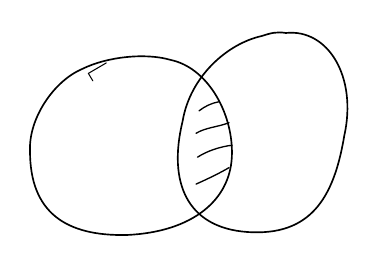
\begin{tikzpicture}[x=.19mm,y=-.19mm,line cap=round,line join=round]
\draw[line width=.6pt] (54,35)
  .. controls (35,43) and (18,68) .. (19,90)
  .. controls (19,131) and (43,147) .. (84,146)
  .. controls (127,144) and (154,123) .. (154,91)
  .. controls (154,63) and (137,34) .. (113,29)
  .. controls (96,24) and (70,27) .. (54,35);
\draw[line width=.6pt] (174,13)
  .. controls (151,18) and (126,40) .. (121,70)
  .. controls (111,111) and (124,141) .. (164,144)
  .. controls (206,147) and (222,122) .. (229,80)
  .. controls (238,40) and (218,8) .. (190,11)
  .. controls (184,10) and (180,11) .. (174,13);
\draw[line width=.38pt] (70,31)--(58,38)--(61,43);
\draw[line width=.48pt]
 (132,63)..controls(136,60)and(140,58)..(145,57)
 (130,78)..controls(137,74)and(144,74)..(152,71)
 (131,94)..controls(137,90)and(146,87)..(154,86)
 (130,112)..controls(139,108)and(147,104)..(152,101);
\end{tikzpicture}}\endgroup}
\end{GelfandAdjacentEvidence}
\begin{GelfandAdjacentEvidence}{GELFAND-P000456}{6}


ф-и перехода из $GL(n,\mathbb Z)$.

Можно постр. \uwave{лок. трив.} рассл. с такими ф-ями перехода.

\SourceFigure{GELFAND-P000456}{complex-bundle-link}{Наклонная черта связывает $H_{\mathbb C}$ с подписью.
\par\smallskip\centering\color{black}
\begingroup\color{black}\GelfandFitDiagram{\begin{tikzpicture}[x=1mm,y=1mm,line cap=round,every node/.style={inner sep=0pt,anchor=base west,font=\scriptsize}]
\node (first) at (0,8) {Это $H_{\mathbb R}$ (или};
\node (hc) at ([xshift=1mm]first.base east) {$H_{\mathbb C}$};
\node at ([xshift=1mm]hc.base east) {в зависимости от слоя)};
\node (label) at ([xshift=5.5mm,yshift=-7mm]hc.base west) {компл. вект. расслоение};
\draw ([xshift=.5mm,yshift=-1.1mm]hc.base east)--([xshift=-.8mm,yshift=1.1mm]label.base west);
\end{tikzpicture}}\endgroup}
\end{GelfandAdjacentEvidence}
\begin{GelfandAdjacentEvidence}{GELFAND-P000456}{7}


\SourceFigure{GELFAND-P000456}{holomorphic-sections-link}{Вертикальная черта ведёт к волнисто подчёркнутой подписи. Прямоугольник справа зачёркнут.
\par\smallskip\centering\color{black}
\begingroup\color{black}\GelfandFitDiagram{\begin{tikzpicture}[x=1mm,y=1mm,line cap=round,every node/.style={inner sep=0pt,font=\scriptsize}]
\node[anchor=base west] at (4,10.5) {$H_{\mathcal O}$};
\draw (14,8.7) rectangle (40,14.6);
\foreach \x in {14.4,17.1,19.8,22.5,25.2,27.9,30.6,33.3,36.0}
  \draw[line width=.37pt] (\x,9) -- ++(3.3,5.3);
\node at (27,11.65) {\sout{\ldots}};
\draw (5.5,7.9)--(5.5,4.5);
\node[anchor=base west] at (0,1) {\uwave{пучок голом. сечений \mbox{$H_{\mathbb C}$}}};
\end{tikzpicture}}\endgroup}
\end{GelfandAdjacentEvidence}
\begin{GelfandAdjacentEvidence}{GELFAND-P000456}{8}

\Unclear{GELFAND-P000456}{o-old-fragment}{В начале зачёркнутой записи возможен знак $H$ с нижним индексом.}
\end{GelfandAdjacentEvidence}
\begin{GelfandAdjacentEvidence}{GELFAND-P000456}{9}

\Incomplete{GELFAND-P000456}{o-cancelled}{Запись внутри прямоугольника под зачёркиванием не разобрана.}
\end{GelfandAdjacentEvidence}

\[
H_{\mathcal O}=H_{\mathbb Z}\otimes_{\mathbb Z}\mathcal O_S.
\]
Имеется естеств. связность (Гаусса-Манина)
\[
\nabla\colon H_{\mathcal O}\longrightarrow
\Omega_S^1\otimes_{\mathcal O_S}H_{\mathcal O}
\qquad\text{($\mathbb C$-лин. гомом.)}
\]
$\Omega_S^1$ — голом. дифф. формы пор. $1$


\Needspace{7\baselineskip}
\begin{GelfandAdjacentEvidence}{GELFAND-P000457}{1}
\SourcePage{GELFAND-P000457}{75}
\underline{опр. связности.}

$1.$ $\mathbb C$-линейность.

$2.$ $\varphi\in\mathcal O_{S,s}$ (ростки), $f\in H_{\mathcal O,s}\Rightarrow$
\[
\Rightarrow\nabla(\varphi f)=\varphi\nabla f+d\varphi\otimes f
\]
\underline{Наша связность.}

Берём лок. тривиализацию\\
и базис из пост. сечений (рассл. $H_{\mathbb Z}$) $u_i$
\[
f=\sum\varphi_i u_i,\qquad\varphi_i\in\mathcal O_S
\]
Тогда
\[
\nabla f=\sum d\varphi_i\otimes u_i
\]
Это опр. корректно и удовл. всем аксиомам.

Кривизна этой связности равна $0$.
\Unclear{GELFAND-P000457}{curvature-sign}{Последний знак читается $0$.}
\end{GelfandAdjacentEvidence}
\begin{GelfandAdjacentEvidence}{GELFAND-P000457}{2}


\underline{Требование на связность Г.-М.}\quad
(\underline{или на} \sout{\ldots}\ \underline{фильтрацию})
\[
\nabla(\mathcal F^p)\subset\Omega_S^1\otimes\mathcal F^{p-1}.
\]
\hfill(Гриффитс)\par
\Unclear{GELFAND-P000457}{filter-old}{Чтение зачёркнутого знака после «или на» не установлено.}
\end{GelfandAdjacentEvidence}
\begin{GelfandAdjacentEvidence}{GELFAND-P000457}{3}


(Задана фильтрация $H_{\mathbb C}=F^0\supset F^1\supset\cdots$)\\
\hspace*{4em}голом. подрасслоениями

$\mathcal F^p$ — пучки сечений $F^p$

\begin{center}
\rule[.5ex]{15mm}{.35pt}\enspace$\cdot$\enspace\rule[.5ex]{22mm}{.35pt}
\end{center}

\uwave{Есть лок. постоянная билин. форма \mbox{$\psi(x,y)$} на \mbox{$H_{\mathbb C}$}}
\Unclear{GELFAND-P000457}{form-letter}{Буква перед $(x,y)$ читается $\psi$.}
\end{GelfandAdjacentEvidence}
\begin{GelfandAdjacentEvidence}{GELFAND-P000457}{4}


\sout{\ldots}
\Incomplete{GELFAND-P000457}{mid-cancelled}{Короткая зачёркнутая запись перед «и» не разобрана.}
\end{GelfandAdjacentEvidence}
\begin{GelfandAdjacentEvidence}{GELFAND-P000457}{5}

и в $\forall$ точке $s\in S$ это структура Ходжа.

\begin{center}
\rule[.5ex]{15mm}{.35pt}\enspace$\cdot$\enspace\rule[.5ex]{22mm}{.35pt}
\end{center}

Пусть $0\le p\le n$,\quad $k_p\ge k_{p+1}$ — послед. чисел
\[
k_0\ge k_1\ge\cdots\ge k_n.
\]
$Z$ — пр-во с элем. $F=\{F^0\supset F^1\supset\cdots\supset F^n\}$,\\
где $\dim F^p=k_p$.
\Unclear{GELFAND-P000457}{dimension-sup}{Показатель $p$ у $F$ густо наведён.}
\end{GelfandAdjacentEvidence}


Это проект. алг. мн-зие.


\Needspace{7\baselineskip}
\begin{GelfandAdjacentEvidence}{GELFAND-P000458}{1}
\SourcePage{GELFAND-P000458}{unlabelled}
\[
H_{\mathbb C}=F^0,\qquad H_{\mathbb Z}\subset H_{\mathbb R}\subset H_{\mathbb C}.
\]
Пусть на $H_{\mathbb C}$ зад. билин. форма $\psi$ (невыр.),
\Unclear{GELFAND-P000458}{first-form}{Знак после «форма» читается $\psi$.}
\end{GelfandAdjacentEvidence}
\begin{GelfandAdjacentEvidence}{GELFAND-P000458}{2}

симм. при неч. $n$ и кос. при чётн. $n$; целочисл.
\Unclear{GELFAND-P000458}{parity-statement}{В рукописи стоит «симм. при неч. $n$ и кос. при чётн. $n$».}
\end{GelfandAdjacentEvidence}
\begin{GelfandAdjacentEvidence}{GELFAND-P000458}{3}


$\overline D$ — подмн. в $Z$ таких флагов, что
\SourceFigure{GELFAND-P000458}{orthogonality-bracket}{Черта охватывает формулу снизу и с двух сторон.
\par\smallskip\centering\color{black}
\begingroup\color{black}\GelfandFitDiagram{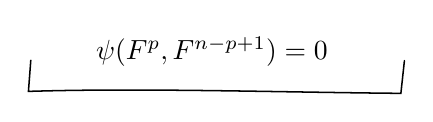
\begin{tikzpicture}[x=1mm,y=1mm,line cap=round]
\node at (25,6.4) {$\psi(F^p,F^{n-p+1})=0$};
\draw[line width=.55pt] (2,5.3)--(1.7,1.35)
  .. controls (16,1.8) and (33,1.25) .. (49,1.1)--(49.45,5.25);
\end{tikzpicture}}\endgroup}
\end{GelfandAdjacentEvidence}
\begin{GelfandAdjacentEvidence}{GELFAND-P000458}{4}


\noindent\rule{\linewidth}{.35pt}

\underline{Доп. усл.}\\
\underline{на флаги}\quad $1)\quad F^p\oplus\overline{F^{n-p+1}}\cong H_{\mathbb C}$
\Unclear{GELFAND-P000458}{sum-formula}{Конец показателя $n-p+1$ густо наведён рядом со знаком $\cong$.}
\end{GelfandAdjacentEvidence}
\begin{GelfandAdjacentEvidence}{GELFAND-P000458}{5}


$2)$ По нему стр. градуировка и автом. Вейля $C$ и тогда
\[
\psi(x,C\bar y)\quad\text{полож. опр. эрм. форма на $H_{\mathbb C}$.}
\]
\Unclear{GELFAND-P000458}{weil-link-full}{После $C$ читается «и тогда».}
\end{GelfandAdjacentEvidence}
\begin{GelfandAdjacentEvidence}{GELFAND-P000458}{6}


Эти условия выделяют $\underset{\text{(открытое).}}{D}\subset\overline D$.

$D$ наз. классиф. пр-вом структур Ходжа.

Зависит от набора размерностей и формы $\psi$.

\underline{След. раз}: однородность.

гр. компл. пр. $H_{\mathbb C}$, сохр. $\psi$, транзит. на $\overline D$

Св. комп. \(\vphantom{G}_{1}\) гр. вещ. пр. $H_{\mathbb R}$, сохр. $\psi$, транзит. на $D$
\Unclear{GELFAND-P000458}{real-prefix}{Слева предположительно «Св. комп.» и опущенный знак, похожий на $1$.}
\end{GelfandAdjacentEvidence}
\begin{GelfandAdjacentEvidence}{GELFAND-P000458}{7}


\medskip\noindent\rule{\linewidth}{.35pt}

\underline{2-я лекция Манина}.

\medskip\noindent\rule{\linewidth}{.35pt}

\uuline{Д: Каждан.}\quad Ещё о раб. Тэйта.
\Unclear{GELFAND-P000458}{footer-heading}{После инициала видны две точки, одна над другой.}



\SourceFigure{GELFAND-P000458}{bottom-mark}{Узкий знак из нескольких штрихов пересекает разделительную черту. Надёжной буквенной подписи или стрелки не видно.
\par\smallskip\centering\color{black}
\begingroup\color{black}\GelfandFitDiagram{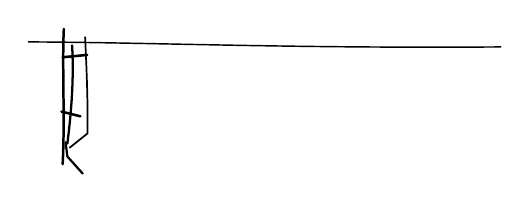
\begin{tikzpicture}[x=.75mm,y=-.75mm,line cap=round,line join=round]
\draw[line width=.52pt] (0,4.6) .. controls (22,4.7) and (43,5.7) .. (80,5.45);
\draw[line width=.9pt] (6,2.4) .. controls (5.7,8.4) and (6.2,18) .. (5.8,25.3);
\draw[line width=.82pt] (7.4,5.2) .. controls (7.8,11.9) and (7,18.6) .. (6.6,21.8);
\draw[line width=.62pt] (9.6,3.8) .. controls (9.9,9.9) and (10.1,15.8) .. (10,20.1)
 -- (7,22.5);
\draw[line width=.92pt] (5.8,7.2)--(9.95,6.8) (5.6,16.4)--(8.8,17.2);
\draw[line width=.8pt] (6.3,21.6)--(6.6,24)--(9.2,26.9);
\end{tikzpicture}}\endgroup}
\end{GelfandAdjacentEvidence}



\Needspace{10\baselineskip}
\section*{Глава 6}

\Needspace{7\baselineskip}
\begin{GelfandAdjacentEvidence}{GELFAND-P000459}{1}
\SourcePage{GELFAND-P000459}{unlabelled}
\uuline{В. Бухштабер.}

\underline{Формальные}\enspace\underline{группы}.

Было опред. формальной группы.

\SourceFigure{GELFAND-P000459}{commutative-insertion}{Сокращение «коммут.» вписано в обведённую выноску над словом «кольцо».
\par\smallskip\centering\color{black}
\begingroup\color{black}\GelfandFitDiagram{\begin{tikzpicture}[x=1mm,y=1mm,line cap=round,line join=round,every node/.style={inner sep=0pt,anchor=base west,font=\small}]
\node (start) at (0,0) {$A$ — произв.};
\node (ring) at ([xshift=1mm]start.base east) {кольцо};
\node at ([xshift=1mm]ring.base east) {с $1$;};
\node (insert) at ([xshift=-1mm,yshift=6.2mm]ring.base west) {коммут.};
\draw ([xshift=-1.2mm,yshift=.6mm]insert.north west)
  .. controls ([xshift=2mm,yshift=1mm]insert.north west)
          and ([xshift=-2mm,yshift=1mm]insert.north east)
       .. ([xshift=1.1mm,yshift=.8mm]insert.north east)
  to[out=0,in=90] ([xshift=2.2mm]insert.east)
  to[out=-90,in=0] ([xshift=.9mm,yshift=-1mm]insert.south east)
  -- ([xshift=2mm,yshift=-1mm]insert.south west)
  -- ([xshift=-.65mm,yshift=.45mm]ring.north west)
  to[out=105,in=-5] ([xshift=-1.6mm,yshift=-.7mm]insert.south west)
  to[out=170,in=-85] ([xshift=-1.2mm,yshift=.6mm]insert.north west);
\end{tikzpicture}}\endgroup}
\end{GelfandAdjacentEvidence}
\begin{GelfandAdjacentEvidence}{GELFAND-P000459}{2}

\[
\sum_{i=0}^{\infty}a_i x^i,\qquad a_i\in A
\]
Форм. группа:
\[
F(x,y)=x+y+\sum_{i+k\ge2}a_{ik}x^iy^k
\]
— форм. степ. ряд.

Условия: ассоциативность, коммутативность (она след. из ассоц.).
Сущ. обр. элем. из теор. о неявной ф-и.
\Unclear{GELFAND-P000459}{inverse-note}{Последние слова читаются «неявной ф-и».}
\end{GelfandAdjacentEvidence}
\begin{GelfandAdjacentEvidence}{GELFAND-P000459}{3}


Изоморфизм:
\[
z=\varphi(x)=x+a_1x^2+\ldots;
\qquad\varphi^{-1}(x)=z-a_1z^2+\ldots
\]
\Unclear{GELFAND-P000459}{change-symbol}{Знак в первой формуле читается $\varphi$.}
\end{GelfandAdjacentEvidence}
\begin{GelfandAdjacentEvidence}{GELFAND-P000459}{4}

\Unclear{GELFAND-P000459}{inverse-symbol}{Перед показателем $-1$ читается тот же знак $\varphi$.}
\end{GelfandAdjacentEvidence}
\begin{GelfandAdjacentEvidence}{GELFAND-P000459}{5}

\Unclear{GELFAND-P000459}{inverse-argument}{В скобках виден $x$, в правой части — $z$.}
\end{GelfandAdjacentEvidence}
\begin{GelfandAdjacentEvidence}{GELFAND-P000459}{6}


\sout{\ldots}\quad и одна получ. из другой заменой переменных.
\Incomplete{GELFAND-P000459}{cancel-before-equivalence}{Запись перед «и одна» зачёркнута. Целое чтение не установлено.}
\end{GelfandAdjacentEvidence}
\begin{GelfandAdjacentEvidence}{GELFAND-P000459}{7}


Будут классифицированы форм. группы (но не с точностью до изом. — это отдельная задача)

Ряд $g(x)=x+\ldots$ наз. логарифмом гр. $F$, если
\[
F(x,y)=g^{-1}(g(x)+g(y))
\]
\underline{Лемма Лазара.}\quad Если $A$ есть $\mathbb Q$-модуль,
то любая форм. группа $F(x,y)$ над $A$ имеет логарифм.
\Unclear{GELFAND-P000459}{lemma-name}{Предположительно «Лазара». Возможное чтение гласной после «з» — «у».}
\end{GelfandAdjacentEvidence}


\underline{Док-во.} (см. Мат., $13:6$)


\Needspace{7\baselineskip}
\begin{GelfandAdjacentEvidence}{GELFAND-P000460}{1}
\SourcePage{GELFAND-P000460}{unlabelled}
Рассм. вместо $A$ кольцо $A[[t]]$; $t$ — время.

Тогда опр. сдвиг \uuline{\mbox{$x\mapsto F(x,t)$}} (сдвиг форм. перем. на время $t$).

Дифференциал:
\[
\omega(x)=\psi(x)\,dx
\]
\Unclear{GELFAND-P000460}{differential-symbol}{Первый знак коэффициента передаётся как $\psi$. Та же буква повторяется в формулах ниже.}
\end{GelfandAdjacentEvidence}
\begin{GelfandAdjacentEvidence}{GELFAND-P000460}{2}


\SourceFigure{GELFAND-P000460}{annotation}{Над формулой тонкой линией выделена приписка.
\par\smallskip\centering\color{black}
\begingroup\color{black}\GelfandFitDiagram{\begin{tikzpicture}[x=1mm,y=1mm,line cap=round,every node/.style={inner sep=0pt,anchor=base west,font=\scriptsize}]
\node (coefficient) at (0,0) {$\psi(x)\in A[[t]][[x]];$};
\node at ([xshift=3mm]coefficient.base east) {$A\subset A[[t]]$};
\node (insert) at (12,6.4) {можно рассм. как элем.};
\draw[line width=.35pt] ([xshift=-.4mm,yshift=-.8mm]insert.south west)
  .. controls ([xshift=4mm,yshift=-.9mm]insert.south west)
          and ([xshift=-3mm,yshift=-.8mm]insert.south east)
       .. ([xshift=1.2mm,yshift=-.9mm]insert.south east)
  to[out=8,in=-84] ([xshift=1.3mm,yshift=.2mm]insert.north east);
\draw[line width=.35pt] ([xshift=-.8mm,yshift=.4mm]insert.west)
  .. controls (11.8,5.8) and (13.9,4.9) .. (12,2.9);
\end{tikzpicture}}\endgroup}
\end{GelfandAdjacentEvidence}
\begin{GelfandAdjacentEvidence}{GELFAND-P000460}{3}


Инв. форма (дифференциал):
\SourceFigure{GELFAND-P000460}{dx-relation}{Два вертикальных штриха и «или» стоят между формулами.
\par\smallskip\centering\color{black}
\begingroup\color{black}\GelfandFitDiagram{\begin{tikzpicture}[x=1mm,y=1mm,every node/.style={inner sep=0pt,anchor=base west,font=\small}]
\node at (0,17) {$\psi(F(x,t))\,dF(x,t)=\psi(x)\,dx.$};
\node at (19,11.3) {\rotatebox{90}{$=$}\ \textnormal{или}};
\node at (2.6,2.5) {$\psi(F(x,t))\,\dfrac{\partial F(x,t)}{\partial x}\,dx$};
\end{tikzpicture}}\endgroup}
\end{GelfandAdjacentEvidence}
\begin{GelfandAdjacentEvidence}{GELFAND-P000460}{4}

\[
\psi(F(x,t))\,\frac{\partial F(x,t)}{\partial x}=\psi(x)
\]
($t$ параметр; дифференциал берётся только по $x$)

Положим $x=0$:
\[
\begin{aligned}
\left.\psi(t)(1+\ldots)\right|_{x=0}&=\psi(0),\\
\psi(t)&=\psi(0)\,\frac{1}{\left.\dfrac{\partial F(x,t)}{\partial x}\right|_{x=0}}.
\end{aligned}
\]
Таковы ряды, явл. коэфф. при инв. дифференциале.

Каноническая форма:
\[
\omega(x)=\frac{1}{\left.\dfrac{\partial F(x,y)}{\partial y}\right|_{y=0}}\,dx
\]
является \sout{\ldots} инвар. дифференциалом (простое упражнение).
\Unclear{GELFAND-P000460}{invariant-mark}{Между словами виден густой вертикальный знак. Его чтение не установлено.}
\end{GelfandAdjacentEvidence}
\begin{GelfandAdjacentEvidence}{GELFAND-P000460}{5}


Это даёт хар-ку.

Рассм. форм. ряд
\[
g(x)=\int_0^x\omega(x)=x+\ldots
\]
(важно, что $A$ есть $\mathbb Q$-модуль! — появляются целые знаменатели при интегрировании)
\Unclear{GELFAND-P000460}{integration-punctuation}{После «модуль» читается восклицательный знак.}
\end{GelfandAdjacentEvidence}
\begin{GelfandAdjacentEvidence}{GELFAND-P000460}{6}

\Unclear{GELFAND-P000460}{integration-margin}{Первое слово после тире читается «появляются».}
\end{GelfandAdjacentEvidence}
\begin{GelfandAdjacentEvidence}{GELFAND-P000460}{7}


Интегрируем соотн.:
\[
\begin{gathered}
\psi(F(x,t))\,dF(x,t)=\psi(x)\,dx\\
g(F(x,y))=g(x)+C;
\end{gathered}
\]
Здесь интегрируется по $x$ ($t$ — пар.), поэтому $C=C(y)$.

Положим $x=0$. Получим: $C=g(y)$ \sout{\ldots}
\Incomplete{GELFAND-P000460}{constant-cancel}{Запись после $C=g(y)$ зачёркнута и не разобрана.}
\end{GelfandAdjacentEvidence}
\begin{GelfandAdjacentEvidence}{GELFAND-P000460}{8}

\[
\begin{gathered}
g(F(x,y))=g(x)+g(y)\\
F(x,y)=g^{-1}(g(x)+g(y)).\quad !!\qquad\blacksquare
\end{gathered}
\]
\uuline{Следствие}\quad Над $\mathbb Q$-мод. все форм. законы сильно изом.

Универс. закон: рассм. $g(x)=x+\sum g_i x^{i+1}$ — ряд, его кольцо $\mathbb Q[g_i]$.
\[
F(x,y)=g^{-1}(g(x)+g(y));
\]
Над $\overset{\downarrow}{\mathbb Q}[g_i]$ получ. универс. закон.
(для всех $\mathbb Q$-модулей)
\Unclear{GELFAND-P000460}{base-ring-overwrite}{Под стрелкой наведена буква $\mathbb Q$. Прежние штрихи не отделяются.}
\end{GelfandAdjacentEvidence}
\begin{GelfandAdjacentEvidence}{GELFAND-P000460}{9}


\begin{center}
\rule[.5ex]{17mm}{.35pt}\enspace$\cdot$\enspace\rule[.5ex]{22mm}{.35pt}
\end{center}

Будем классиф. над произв. кольцами $A$ (коммут. и с $1$)
\Unclear{GELFAND-P000460}{universal-verb}{Первое слово читается «Будем».}
\end{GelfandAdjacentEvidence}
\begin{GelfandAdjacentEvidence}{GELFAND-P000460}{10}


\SourceFigure{GELFAND-P000460}{universal-arrow}{Дуга со стрелкой идёт от записи универсального закона к скобке перед «Универсальность».
\par\smallskip\centering\color{black}
\begingroup\color{black}\GelfandFitDiagram{\begin{tikzpicture}[x=1mm,y=1mm,line cap=round]
\draw[->,line width=.6pt] (6,17) .. controls (1,14) and (.5,7) .. (2.1,2.6);
\draw[line width=.5pt] (4.7,4.05)--(3.7,4.05)--(3.7,.35)--(4.7,.35);
\node[anchor=base west,inner sep=0pt,font=\small] at (5.4,1) {Универсальность:};
\end{tikzpicture}}\endgroup}
\end{GelfandAdjacentEvidence}
\begin{GelfandAdjacentEvidence}{GELFAND-P000460}{11}

любой ряд $F(x,y)$ над $\mathbb Q$-мод. $A$ получ. из такого заменой коэффициентов их гомоморфными образами при гомом. кольца
$\mathbb Q[g_i]$ в $A$, перевод. $g_i$ в коэфф. ряда $g(x)$,
найденные выше\(\bigr]\)
\Unclear{GELFAND-P000460}{universal-images}{Окончания обоих слов читаются во множественном числе «гомоморфными образами».}
\end{GelfandAdjacentEvidence}



\Needspace{7\baselineskip}
\begin{GelfandAdjacentEvidence}{GELFAND-P000461}{1}
\SourcePage{GELFAND-P000461}{unlabelled}
\underline{Рассм. теперь общий случай}: $A$ не обяз. $\mathbb Q$-модуль.

Рассм. ряд $F(x,y)=x+y+\sum a_{i,j}x^iy^j$

$a_{i,j}$ — алг. независ. переменные.

Рассм. $\mathbb Z[a_{i,j}]$,\quad $\deg a_{i,j}=i+j-1$

Из него получ. форм. группа
\[
\begin{gathered}
F(F(x,y),z)=x+y+z+\sum a_{i,j,k}x^iy^jz^k,\quad
a_{i,j,k}\in\mathbb Z[a_{i,j}].\\
F(x,F(y,z))=x+y+z+\sum a'_{i,j,k}x^iy^jz^k
\qquad a'_{i,j,k}\in\mathbb Z[a_{i,j}]
\end{gathered}
\]
Рассм. в $\overset{\mathbb Z[a_{i,j}]}{\text{\sout{\ldots}}}$ идеал
$J$, порожд. однор. элем. $\{a_{i,j,k}-a'_{i,j,k}\}$
и элементами $\{a_{i,j}-a_{j,i}^{\text{\sout{\ldots}}}\}$.
\Incomplete{GELFAND-P000461}{ideal-cancel}{Над зачёркнутой записью вписано $\mathbb Z[a_{i,j}]$. Прежняя запись не разобрана.}
\end{GelfandAdjacentEvidence}
\begin{GelfandAdjacentEvidence}{GELFAND-P000461}{2}

\Unclear{GELFAND-P000461}{comm-coefficient}{Над вторым коэффициентом $a_{j,i}$ остались зачёркнутые штрихи.}
\end{GelfandAdjacentEvidence}
\begin{GelfandAdjacentEvidence}{GELFAND-P000461}{3}


Теперь заменим $a_{i,j}$ в $F(x,y)$ на $a_{i,j}\bmod J$ —
\sout{\ldots} получим ряд $F\in\Lambda[[x,y]]$.
\Incomplete{GELFAND-P000461}{cancel-before-series}{Запись перед «получим» зачёркнута и не разобрана.}
\end{GelfandAdjacentEvidence}
\begin{GelfandAdjacentEvidence}{GELFAND-P000461}{4}

\[
\Lambda=\mathbb Z[a_{i,j}]/J
\]
Это универс. группа. (ясно).

\underline{Теор. Лазара}, $\Lambda$ — кольцо полиномов от образующих по одной в каждой размерности:
\[
\Lambda=\mathbb Z[a_i],\quad i\ge1,\quad\deg a_i=i.
\]
\Unclear{GELFAND-P000461}{one-generator-overwrite}{В слове «одной» предпоследняя буква густо наведена.}
\end{GelfandAdjacentEvidence}
\begin{GelfandAdjacentEvidence}{GELFAND-P000461}{5}


По \underline{лемме Лазара}:
\SourceFigure{GELFAND-P000461}{rational-identity-divider}{Две пары черт с точками расположены над и под равенством.
\par\smallskip\centering\color{black}
\begingroup\color{black}\GelfandFitDiagram{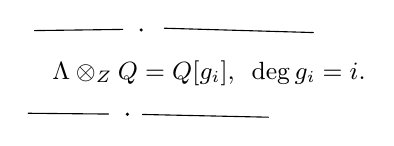
\begin{tikzpicture}[x=1mm,y=1mm,line cap=round,every node/.style={inner sep=0pt,anchor=base west,font=\small}]
\node (eq) at (3,0) {$\Lambda\otimes_{\mathbb Z}\mathbb Q=\mathbb Q[g_i],$};
\node at ([xshift=2mm]eq.base east) {$\deg g_i=i$.};
\draw (.8,6.2)--(12,6.35) (17.3,6.5)--(36.2,5.95)
      (0,-4.3)--(10.2,-4.4) (14.5,-4.45)--(30.5,-4.8);
\fill (14.35,6.28) circle (.22) (12.6,-4.42) circle (.22);
\end{tikzpicture}}\endgroup}
\end{GelfandAdjacentEvidence}
\begin{GelfandAdjacentEvidence}{GELFAND-P000461}{6}


\underline{1.}\quad Сколько мульт. образующих имеет $\Lambda$?

Рассм. $\widetilde\Lambda=\Lambda/(\text{разложимым элементам})$.
\Unclear{GELFAND-P000461}{decomposable-word}{Слово в знаменателе предположительно «разложимым».}
\end{GelfandAdjacentEvidence}
\begin{GelfandAdjacentEvidence}{GELFAND-P000461}{7}


\SourceFigure{GELFAND-P000461}{indecomposable-ideal-link}{Короткая вертикальная черта соединяет первое кольцо с пояснением.
\par\smallskip\centering\color{black}
\begingroup\color{black}\GelfandFitDiagram{\begin{tikzpicture}[x=1mm,y=1mm,line cap=round,every node/.style={inner sep=0pt,anchor=base west,font=\small}]
\node (ring) at (0,15) {$\mathbb Z[a_{i,j}]$};
\node at ([xshift=1mm]ring.base east) {$\longrightarrow\Lambda\longrightarrow0$.};
\node[anchor=north west,text width=51mm,align=left] at (2,5.8) {здесь есть идеал, порожд. разл. элем. (произв. $2$-х ненулев. степени)};
\draw (6.2,10.4)--(6.15,7.1);
\end{tikzpicture}}\endgroup}
\end{GelfandAdjacentEvidence}
\begin{GelfandAdjacentEvidence}{GELFAND-P000461}{8}


\noindent
\begin{tabular}{@{}p{.44\linewidth}@{\hspace{2mm}}||@{\hspace{2mm}}p{.49\linewidth}@{}}
\raggedright Имеем: $\widetilde\Lambda=\sum_{i\ge0}\widetilde\Lambda_i$;\par
умножение — нулевое, кроме случая, когда один из \sout{\ldots} $0$-й элем. &
\raggedright Разлож. элем. — элем. вида $a\cdot b$, где $a$ и $b$ \({}^{\ast}\)\par
\({}^{\ast}\) необратимы. Берется идеал, ими порождённый, и $\widetilde\Lambda$ — факторкольцо.\par
Градуировка $\Rightarrow$ обратимы только элем. $0$-й степ.\par
Отсюда идеал этот — образ идеала разл. эл. из $\mathbb Z[a_{i,j}]$.\tabularnewline
\end{tabular}
\SourceFigure{GELFAND-P000461}{margin-layout}{Две вертикальные черты отделяют правую приписку.}
\end{GelfandAdjacentEvidence}
\begin{GelfandAdjacentEvidence}{GELFAND-P000461}{9}

\Unclear{GELFAND-P000461}{graded-sum-glyph}{Слева от равенства, вероятно, $\widetilde\Lambda$ со слитной тильдой. Возможное чтение — $\chi$.}
\end{GelfandAdjacentEvidence}
\begin{GelfandAdjacentEvidence}{GELFAND-P000461}{10}

\Incomplete{GELFAND-P000461}{pi-degree-zero}{Короткая запись после «из» зачёркнута и не разобрана.}
\end{GelfandAdjacentEvidence}
\begin{GelfandAdjacentEvidence}{GELFAND-P000461}{11}

\Unclear{GELFAND-P000461}{margin-nonunits}{В правой приписке читается «необратимы».}
\end{GelfandAdjacentEvidence}
\begin{GelfandAdjacentEvidence}{GELFAND-P000461}{12}

\Unclear{GELFAND-P000461}{margin-verb}{После «необратимы» читается «Берется».}
\end{GelfandAdjacentEvidence}
\begin{GelfandAdjacentEvidence}{GELFAND-P000461}{13}


$\widetilde\Lambda_n$ — абелева гр. по слож. с образующ. — обр. мульт. гр. $\Lambda$ в размерности $n$.
\[
F(F(x,y),z)=F(x,y)+z+\sum a_{i,j}\,\text{\sout{\ldots}}\,(x+y)^i z^j
\]
\Incomplete{GELFAND-P000461}{cancel-exponent}{Запись перед $(x+y)^i$ зачёркнута и не разобрана.}
\end{GelfandAdjacentEvidence}
\begin{GelfandAdjacentEvidence}{GELFAND-P000461}{14}


\SourceFigure{GELFAND-P000461}{product-insertion}{В обведённую выноску над строкой вписано «разных $a_{i,j}$».
\par\smallskip\centering\color{black}
\begingroup\color{black}\GelfandFitDiagram{\begin{tikzpicture}[x=1mm,y=1mm,line cap=round,line join=round,every node/.style={inner sep=0pt,anchor=base west,font=\small}]
\node (prod) at (0,0) {(в $\widetilde\Lambda$ произведение};
\node (rest) at ([xshift=1.2mm]prod.base east) {уже равно $0$).};
\node (insert) at ([xshift=-6mm,yshift=6.5mm]rest.base west) {разных $a_{i,j}$};
\draw ([xshift=-1.6mm,yshift=.9mm]insert.north west)
   -- ([xshift=1.4mm,yshift=.9mm]insert.north east)
   to[out=0,in=90] ([xshift=2.2mm]insert.east)
   to[out=-90,in=0] ([xshift=1.3mm,yshift=-1.2mm]insert.south east)
   -- ([xshift=6.5mm,yshift=-1mm]insert.south west)
   to[out=180,in=86] ([xshift=-.4mm,yshift=.55mm]rest.north west)
   to[out=90,in=0] ([xshift=4mm,yshift=-1mm]insert.south west)
   -- ([xshift=-1.6mm,yshift=-1mm]insert.south west)
   -- cycle;
\end{tikzpicture}}\endgroup}
\end{GelfandAdjacentEvidence}

\[
F(x,F(y,z))=x+F(y,z)+\sum a_{i,j}x^i(y+z)^j
\]
$\widetilde\Lambda$ получ. из своб. аб. группы, порожд. $a_{i,j}$, профакториз. по соотн. \ldots

Пусть $h(x,y)=\sum h_{i,j}x^iy^j=F(x,y)-x-y$.
\[
h(x,0)=0,\quad h(0,y)=0.
\]


\Needspace{7\baselineskip}
\begin{GelfandAdjacentEvidence}{GELFAND-P000462}{1}
\SourcePage{GELFAND-P000462}{unlabelled}
Соотн. Лазара:
\[
\uwave{\mbox{$h(x,y)+h(x+y,z)=h(y,z)+h(x,y+z).$}}\qquad(*)
\]
Дост. брать однор. многочлены $h$.

У Лазара: методы теории чисел.

\uwave{Задача:}\quad найти все решения $(*)$ [однор. многочл.] над нек-рым кольцом $K$.

Все решения — \uwave{группа \mbox{$L$}},\quad Всё над кольцом $K$
\[
L\longrightarrow\operatorname{Ext}_{K[x]}^{2,n}(K,K)\longrightarrow0.
\]
Введём в $K[x]$ структ. Хопфа: мульт. гомоморфизм
\[
\begin{gathered}
\Delta:K[x]\longrightarrow K[x]\otimes_K K[x]\qquad\text{(косложение).}\\
x\longrightarrow x\otimes1+1\otimes x
\end{gathered}
\]
У алг. Хопфа есть когомологии. Алг. градуир. $\Rightarrow$ когом. биградуир.
Отсюда $2$ индекса у $\operatorname{Ext}$.

Далее:
\[
\begin{aligned}
 &\quad\text{слева и справа}\quad (x+y+z)^n-x^n-y^n-z^n\\[-.2ex]
 &\qquad\downarrow\\[-.2ex]
 0&\longrightarrow
 \{c((x+y)^n-x^n-y^n),\,a\in K\}
 \longrightarrow L\longrightarrow
 \operatorname{Ext}_{K[x]}^{2,n}(K,K)\longrightarrow0.
\end{aligned}
\]
\SourceFigure{GELFAND-P000462}{sequence-arrow}{Стрелка от приписки направлена вниз к первому члену последовательности.}
\end{GelfandAdjacentEvidence}
\begin{GelfandAdjacentEvidence}{GELFAND-P000462}{2}

\Unclear{GELFAND-P000462}{family-coefficient}{Перед скобками предположительно $c$. Отдельно написано $a\in K$. Оба знака густо наведены.}
\end{GelfandAdjacentEvidence}
\begin{GelfandAdjacentEvidence}{GELFAND-P000462}{3}


\begin{center}
\rule[.5ex]{17mm}{.35pt}\enspace$\cdot$\enspace\rule[.5ex]{22mm}{.35pt}
\end{center}

\uuline{\mbox{$n=2$}}.\quad
$\overset{\text{\sout{\ldots}}}{\text{Многочл.}}$ $2$-й степени
\uuline{\mbox{$cxy$}}.
\Unclear{GELFAND-P000462}{cancel-n2}{Знак над «Многочл.» зачёркнут и не разобран.}
\end{GelfandAdjacentEvidence}
\begin{GelfandAdjacentEvidence}{GELFAND-P000462}{4}


\uuline{\mbox{$n=3$}}\quad $h(x,y)=C_1x^2y+C_2xy^2$
\[
\widetilde\Lambda=\mathbb Z+\mathbb Z_3.
\]
\Unclear{GELFAND-P000462}{cubic-quotient}{Читается $\widetilde\Lambda=\mathbb Z+\mathbb Z_3$.}
\end{GelfandAdjacentEvidence}
\begin{GelfandAdjacentEvidence}{GELFAND-P000462}{5}


$1$ реш. по лемме Лазара: $c((x+y)^n-x^n-y^n)$

$h(x,y)=x^2y+xy^2$\qquad для всех колец

$h(x,y)=x^2y$\qquad для колец, явл. $\mathbb Z_3$-модулями
\Unclear{GELFAND-P000462}{cubic-module-claim}{В этой строке у $\mathbb Z$ нижний индекс $3$.}
\end{GelfandAdjacentEvidence}
\begin{GelfandAdjacentEvidence}{GELFAND-P000462}{6}


\noindent\hspace*{1.7em}$x^2y$

\begin{center}
\rule[.5ex]{26mm}{.35pt}\enspace$\cdot$\enspace\rule[.5ex]{27mm}{.35pt}
\end{center}
Рассм. комодули над алг. Хопфа $A$ — это аб. гр. $N$, для к-рой есть отобр. $N\longrightarrow A\otimes N$ с ест. усл.
\begin{center}
\rule[.5ex]{25mm}{.35pt}\enspace$\cdot$\enspace\rule[.5ex]{29mm}{.35pt}
\end{center}

Надо прав. подобр. резольвенту: будут все циклы без границ (миним. резольвента). \sout{по}
\Unclear{GELFAND-P000462}{cancel-after-resolution}{Под зачёркиванием после скобки предположительно «по».}
\end{GelfandAdjacentEvidence}
\begin{GelfandAdjacentEvidence}{GELFAND-P000462}{7}

\begin{center}
\rule[.5ex]{26mm}{.35pt}\enspace$\cdot$\enspace\rule[.5ex]{29mm}{.35pt}
\end{center}

\sout{Н\ldots}
\Unclear{GELFAND-P000462}{cancel-heading-fragment}{В начале зачёркнутого заголовка видна «Н».}
\end{GelfandAdjacentEvidence}
\begin{GelfandAdjacentEvidence}{GELFAND-P000462}{8}

\Incomplete{GELFAND-P000462}{cancel-heading-remainder}{Остальная часть зачёркнутого заголовка не разобрана.}
\end{GelfandAdjacentEvidence}
\begin{GelfandAdjacentEvidence}{GELFAND-P000462}{9}


\uuline{Подсчёт группы \mbox{$\operatorname{Ext}^2$}.}

$1^\circ$. $K$ — \sout{\ldots} комодуль над алг. Хопфа $K[x]$.
\Unclear{GELFAND-P000462}{cancel-comodule}{Между тире после $K$ и «комодуль» зачёркнут густой прямоугольный знак.}
\end{GelfandAdjacentEvidence}
\begin{GelfandAdjacentEvidence}{GELFAND-P000462}{10}


\hfill\sout{\ldots}\quad $x\longrightarrow x\otimes1+1\otimes x$\par
\Unclear{GELFAND-P000462}{coproduct-mark}{Перед $x$ в приписке виден густо перечёркнутый знак.}
\end{GelfandAdjacentEvidence}
\begin{GelfandAdjacentEvidence}{GELFAND-P000462}{11}

\[
K\longrightarrow K\otimes K[x]\quad
\text{\sout{\mbox{$\gets$}\ldots}}
\]
\Unclear{GELFAND-P000462}{cancel-after-tensor-fragment}{Начало зачёркнутой приписки похоже на $\gets$.}
\end{GelfandAdjacentEvidence}
\begin{GelfandAdjacentEvidence}{GELFAND-P000462}{12}

\Incomplete{GELFAND-P000462}{cancel-after-tensor-remainder}{Остальные штрихи после $K[x]$ не разобраны.}
\end{GelfandAdjacentEvidence}


$1\longrightarrow1\otimes1$\qquad и дальше по линейности.


\Needspace{7\baselineskip}
\begin{GelfandAdjacentEvidence}{GELFAND-P000463}{1}
\SourcePage{GELFAND-P000463}{unlabelled}
Рассм.
\[
K_*[x]=\operatorname{Hom}_K(K[x],K).
\]
(«дифф. операторы»).
\[
(x_*^n,x^m)=\delta_{n,m}
\]
Умножение:
\[
\underline{x_*^n\cdot x_*^m=C_{n+m}^n x_*^{n+m}}
\qquad\text{— \underline{таблица}.}
\]
Здесь $K$ не участвует.

Дост. считать $K=\mathbb Z_p$ или $\mathbb Q$.
\[
K_*[x]=\prod_{q=1}^\infty B_q,\qquad
B_q=\mathbb Z_p[y_{p^i}]/(y_{p^i}^{\,p})
\]
\Unclear{GELFAND-P000463}{product-factorization}{Слева написано $K_*[x]$. У знака произведения нижний предел $q=1$ и верхний $\infty$.}
\end{GelfandAdjacentEvidence}
\begin{GelfandAdjacentEvidence}{GELFAND-P000463}{2}


$y_1,\ldots,y_i,\ldots,y_{p^i}$ — образующие.
\Unclear{GELFAND-P000463}{generator-powers}{В трёх местах $i$ при $p$ приподнят. Набрано $y_{p^i}$. В знаменателе у $y$ отдельно стоит верхняя степень $p$.}
\end{GelfandAdjacentEvidence}



\Needspace{7\baselineskip}
\begin{GelfandAdjacentEvidence}{GELFAND-P000464}{1}
\SourcePage{GELFAND-P000464}{unlabelled}
\underline{30/\mbox{$\overline{\underline{\mathrm X}}$}-72г.}
\quad\underline{Сем. Гельфанда.}

\underline{И. Бернштейн}

\uuline{И.М.Г.}

\SourceFigure{GELFAND-P000464}{general-graph}{Две стрелки слева направлены к общему узлу. Из среднего узла идут стрелки влево, вправо и вниз вправо. Справа видна ломаная с наконечниками. Мелкие штрихи в узлах не прочитаны как буквы.
\par\smallskip\centering\color{black}
\begingroup\color{black}\GelfandFitDiagram{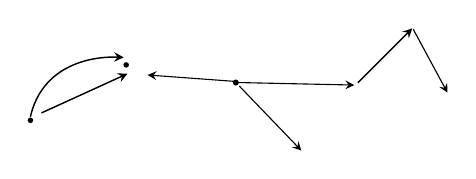
\begin{tikzpicture}[x=.16mm,y=-.16mm,line cap=round,line join=round,>=stealth]
\fill (20,91) circle (1pt) (96,47) circle (1pt) (183,61) circle (1.1pt);
\draw[->,line width=.52pt] (20,88)
 .. controls (29,49) and (65,40) .. (94,41);
\draw[->,line width=.52pt] (29,85)--(97,54);
\draw[->] (181,60)--(113,55);
\draw[->] (185,61)--(277,63);
\draw[->] (186,64)--(235,115);
\draw[->,line width=.5pt] (280,61)--(323,18);
\draw[->] (324,19)--(351,69);
\end{tikzpicture}}\endgroup}
\end{GelfandAdjacentEvidence}
\begin{GelfandAdjacentEvidence}{GELFAND-P000464}{2}


Есть ориентированный граф. Это категория.

\sout{Р}\quad Рассм. какие л. диаграммы, где в точках — вект. пр-ва,
на стрелках отобр. (функторность не требуется).
\Unclear{GELFAND-P000464}{cancel-before-consider}{В начале зачёркнутого знака видна петля. Возможно «Р».}
\end{GelfandAdjacentEvidence}
\begin{GelfandAdjacentEvidence}{GELFAND-P000464}{3}

\Unclear{GELFAND-P000464}{diagram-adjective}{Перед «диаграммы» предположительно «какие л.».}
\end{GelfandAdjacentEvidence}
\begin{GelfandAdjacentEvidence}{GELFAND-P000464}{4}


Зад. — классифицировать.

\SourceFigure{GELFAND-P000464}{one-arrow}{Между двумя точками проведена слегка выгнутая стрелка вправо.
\par\smallskip\centering\color{black}
\begingroup\color{black}\GelfandFitDiagram{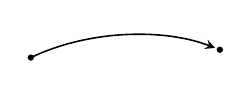
\begin{tikzpicture}[x=1mm,y=1mm,line cap=round,>=stealth]
\fill (0,0) circle (1.15pt) (24,1) circle (1.15pt);
\draw[->,line width=.57pt,shorten >=.65mm] (0,0)
  .. controls (7.5,3.6) and (17,3.7) .. (24,1);
\end{tikzpicture}}\endgroup}
\end{GelfandAdjacentEvidence}
\begin{GelfandAdjacentEvidence}{GELFAND-P000464}{5}


Зад. о классиф. отобр.\quad Инв. лишь $\dim\operatorname{Ker}$ и $\dim\operatorname{Coker}$.
Свод. к вложению.

\SourceFigure{GELFAND-P000464}{one-loop}{Одна петля. Наконечник на её левой стороне направлен вверх.
\par\smallskip\centering\color{black}
\begingroup\color{black}\GelfandFitDiagram{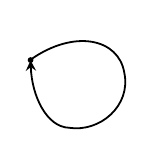
\begin{tikzpicture}[x=1mm,y=1mm,line cap=round,line join=round,>=stealth]
\fill (0,1.4) circle (1.05pt);
\draw[->,line width=.65pt] (0,1.45)
  .. controls (5.6,5.4) and (11.2,4.1) .. (11.9,-.2)
  .. controls (12.8,-4.4) and (8.8,-7.8) .. (4.9,-7.2)
  .. controls (2,-7.1) and (.15,-3.1) .. (0,1.35);
\end{tikzpicture}}\endgroup}
\end{GelfandAdjacentEvidence}
\begin{GelfandAdjacentEvidence}{GELFAND-P000464}{6}


одно преобр.

\SourceFigure{GELFAND-P000464}{two-loop}{Две петли с общим левым узлом. Верхняя часть внешней дуги бледная. Возле узла видны наложенные штрихи наконечников.
\par\smallskip\centering\color{black}
\begingroup\color{black}\GelfandFitDiagram{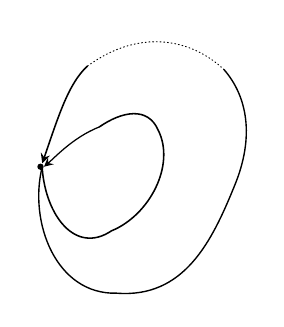
\begin{tikzpicture}[x=.22mm,y=-.22mm,line cap=round,line join=round,>=stealth]
\fill (20,83) circle (1.15pt);
\draw[line width=.5pt] (21,83)
 .. controls (13,115) and (29,157) .. (64,156)
 .. controls (103,159) and (119,126) .. (132,94)
 .. controls (144,65) and (139,42) .. (126,27);
\draw[densely dotted,line width=.34pt] (126,27)
 .. controls (107,9) and (77,3) .. (47,25);
\draw[->,line width=.56pt] (47,25)
 .. controls (36,35) and (30,55) .. (21,81);
\draw[line width=.56pt] (21,84)
 .. controls (23,111) and (40,134) .. (61,120)
 .. controls (83,111) and (98,82) .. (88,62)
 .. controls (82,48) and (67,51) .. (54,60);
\draw[->,line width=.45pt] (54,60) .. controls (39,66) and (29,77) .. (22,83);
\end{tikzpicture}}\endgroup}
\end{GelfandAdjacentEvidence}
\begin{GelfandAdjacentEvidence}{GELFAND-P000464}{7}


— зад. неразрешима (пара произв. лин. операторов). \sout{\ldots}
\Unclear{GELFAND-P000464}{cancel-before-ona}{Короткая запись перед «Она» зачёркнута и не разобрана.}
\end{GelfandAdjacentEvidence}
\begin{GelfandAdjacentEvidence}{GELFAND-P000464}{8}


Она свод. к зад. о коммутирующих (Гельф. и Пономарёв).
\Unclear{GELFAND-P000464}{wild-name}{Первая буква наведена. Сокращение читается «Гельф.».}
\end{GelfandAdjacentEvidence}
\begin{GelfandAdjacentEvidence}{GELFAND-P000464}{9}


\sout{Свод.\ldots}
\Unclear{GELFAND-P000464}{large-cancel-fragment}{Начало зачёркнутой строки предположительно «Свод.».}
\end{GelfandAdjacentEvidence}
\begin{GelfandAdjacentEvidence}{GELFAND-P000464}{10}

\Incomplete{GELFAND-P000464}{large-cancel-remainder}{Остальная зачёркнутая строка не разобрана.}
\end{GelfandAdjacentEvidence}
\begin{GelfandAdjacentEvidence}{GELFAND-P000464}{11}


\[
\left.
\begin{gathered}
\text{Пр-во и подпр-во.}\\
\text{Пр-во и 2 подпр-ва}
\end{gathered}
\right\}\quad\text{трив.}
\]
Делается:\quad пр-во и \uwave{\mbox{$3$} лин. подпр-ва}.
\Unclear{GELFAND-P000464}{three-space-word}{Начало строки предположительно «Делается».}
\end{GelfandAdjacentEvidence}
\begin{GelfandAdjacentEvidence}{GELFAND-P000464}{12}


Инвариантов $9$, а не $8$!

\SourceFigure{GELFAND-P000464}{three-inward}{Три стрелки направлены к верхнему узлу. Их наконечники частично сливаются.
\par\smallskip\centering\color{black}
\begingroup\color{black}\GelfandFitDiagram{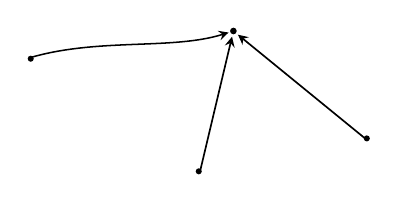
\begin{tikzpicture}[x=.22mm,y=-.22mm,line cap=round,>=stealth]
\fill (22,45) circle (1.1pt) (139,29) circle (1.2pt)
      (119,110) circle (1.1pt) (216,91) circle (1.1pt);
\draw[->,line width=.55pt,shorten >=.65mm] (23,44)
 .. controls (62,33) and (104,40) .. (139,29);
\draw[->,line width=.6pt,shorten >=.75mm] (120,109)--(139,29);
\draw[->,line width=.6pt,shorten >=.75mm] (215,91)--(139,29);
\end{tikzpicture}}\endgroup}
\end{GelfandAdjacentEvidence}
\begin{GelfandAdjacentEvidence}{GELFAND-P000464}{13}

(задача).

\SourceFigure{GELFAND-P000464}{four-inward}{Четыре луча сходятся к густому центральному узлу. Направления двух лучей из-за наложения штрихов не установлены.
\par\smallskip\centering\color{black}
\begingroup\color{black}\GelfandFitDiagram{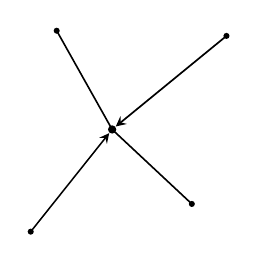
\begin{tikzpicture}[x=.22mm,y=-.22mm,line cap=round,>=stealth]
\fill (31,30) circle (1.1pt) (129,33) circle (1.1pt)
      (16,146) circle (1.1pt) (109,130) circle (1.1pt)
      (63,87) circle (1.5pt);
\draw[line width=.58pt] (31,30)--(63,87)--(109,130);
\draw[->,line width=.61pt,shorten >=.6mm] (129,33)--(63,87);
\draw[->,line width=.55pt,shorten >=.6mm] (16,146)--(63,87);
\end{tikzpicture}}\endgroup}
\end{GelfandAdjacentEvidence}
\begin{GelfandAdjacentEvidence}{GELFAND-P000464}{14}


Пр-во и $4$ подпр-ва классиф. (Гельф. и Поном.) —
\sout{\ldots} уже беск. число неразл.
\Incomplete{GELFAND-P000464}{cancel-after-names}{Слово после тире зачёркнуто и не разобрано.}
\end{GelfandAdjacentEvidence}


\underline{Габриэль}: в каких графах конечное число неразл. систем?

Ответ: нарисовать схему Дынкина! — они и только они явл. такими графами.

Исключения: схемы с двойными (вообще кратными) стрелками.


\Needspace{7\baselineskip}
\begin{GelfandAdjacentEvidence}{GELFAND-P000465}{1}
\SourcePage{GELFAND-P000465}{unlabelled}
\underline{Теорема}\quad
(\begin{tabular}[t]{@{}c@{}}Ройтов\\[-.45ex]\scriptsize из Киева\end{tabular}
или Назаровы).
\Unclear{GELFAND-P000465}{theorem-names}{Фамилии предположительно «Ройтов» и «Назаровы». Под первой строкой приписано «из Киева».}
\end{GelfandAdjacentEvidence}
\begin{GelfandAdjacentEvidence}{GELFAND-P000465}{2}


Опис. класс схем, где есть классифик. как у Гельф. и Пономарёва.

\uwave{Связь \sout{\ldots}\ с особенностями!}\quad — см. Артин, Тюрина, Брискорн.
\Incomplete{GELFAND-P000465}{cancel-specialities}{Слово между «Связь» и «с особенностями» зачёркнуто и не разобрано.}
\end{GelfandAdjacentEvidence}
\begin{GelfandAdjacentEvidence}{GELFAND-P000465}{3}


\begin{center}
\rule[.5ex]{18mm}{.35pt}\enspace$\cdot$\enspace\rule[.5ex]{25mm}{.35pt}
\end{center}

\uuline{И.Б.}\quad \uwave{Категория} вект. пр-в над точками и отобр. над стрелками.

(Граф фиксирован). \quad \uwave{Опред. прямая сумма}. Это $\operatorname{Cat}(\Gamma)$
($\Gamma$ — граф)

Морфизмы — отобр. над каждой точкой с коммут. диагр.

$\bullet$\qquad категория линейных пространств.

Важно: не обязательно отожд. изоморфные.
\Unclear{GELFAND-P000465}{important-line}{Сокращение перед «изоморфные» предположительно «отожд.».}
\end{GelfandAdjacentEvidence}
\begin{GelfandAdjacentEvidence}{GELFAND-P000465}{4}


Легко видеть, что $\forall$ объект $=\sum$ неразлож. (однозн. с точн. до изом.).

$1)$\quad \uwave{Классиф. \mbox{$\Gamma$}, в к-рых конечное число неразл. объектов.}

\underline{Огранич. связными}:

\SourceFigure{GELFAND-P000465}{dynkin-a-mark}{У третьей левой вершины над горизонтальной линией виден маленький угловой штрих.
\par\smallskip\centering\color{black}
\begingroup\color{black}\GelfandFitDiagram{\begin{tikzpicture}[x=.079mm,y=-.079mm,line cap=round,every node/.style={font=\scriptsize,inner sep=0pt}]
\node at (52,58) {$A_n$};
\draw[line width=.58pt] (177,62)--(249,65)--(330,65)--(405,59);
\draw[line width=.58pt] (577,56)--(697,59);
\foreach \x/\y in {177/62,249/65,330/65,697/59}{\fill (\x,\y) circle (1.06pt);}
\foreach \x/\y in {450/65,489/65,527/62}{\fill (\x,\y) circle (.44pt);}
\draw[line width=.44pt] (319,64)--(326,50)--(320,50) (324,51)--(334,47);
\node[anchor=west] at (827,56) {($n$ точек)};
\end{tikzpicture}}\endgroup}
\end{GelfandAdjacentEvidence}
\begin{GelfandAdjacentEvidence}{GELFAND-P000465}{5}


\SourceFigure{GELFAND-P000465}{dynkin-d}{На отрезке между третьей и четвёртой вершинами виден небольшой наконечник влево.
\par\smallskip\centering\color{black}
\begingroup\color{black}\GelfandFitDiagram{\begin{tikzpicture}[x=.074mm,y=-.074mm,line cap=round,every node/.style={font=\scriptsize,inner sep=0pt}]
\node at (50,63) {$D_n$};
\draw[line width=.57pt] (164,64)--(253,63)--(328,66);
\draw[line width=.57pt] (346,65)--(402,63)--(445,64);
\draw[line width=.43pt] (348,61)--(341,65)--(348,69);
\draw[line width=.57pt] (603,67)--(696,65)--(774,21) (696,65)--(764,118);
\foreach \x/\y in {164/64,253/63,328/66,402/63,603/67,696/65,774/21,764/118}
  {\fill (\x,\y) circle (1.04pt);}
\foreach \x/\y in {459/72,496/67,525/67}{\fill (\x,\y) circle (.47pt);}
\node[anchor=west] at (1010,66) {$n\ge4$};
\end{tikzpicture}}\endgroup}
\end{GelfandAdjacentEvidence}
\begin{GelfandAdjacentEvidence}{GELFAND-P000465}{6}


\SourceFigure{GELFAND-P000465}{dynkin-e}{На горизонтальной цепи шесть узлов. От третьего узла слева отходит ветвь вниз.
\par\smallskip\centering\color{black}
\begingroup\color{black}\GelfandFitDiagram{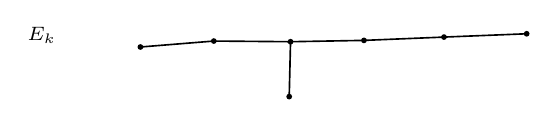
\begin{tikzpicture}[x=.084mm,y=-.084mm,line cap=round,every node/.style={font=\scriptsize,inner sep=0pt}]
\node at (45,53) {$E_k$};
\draw[line width=.59pt] (194,70)--(305,61)--(421,62)--(532,60)--(653,55)--(778,50);
\draw[line width=.6pt] (421,62)--(419,145);
\foreach \x/\y in {194/70,305/61,421/62,532/60,653/55,778/50,419/145}
  {\fill (\x,\y) circle (1.04pt);}
\end{tikzpicture}}\endgroup}
\end{GelfandAdjacentEvidence}
\begin{GelfandAdjacentEvidence}{GELFAND-P000465}{7}

$k=6,7,8$\qquad (слева обязательно $2$ отрезка).

Стрелки расставл. произвольно!!

$D_4$ — пр-во и $3$ подпр-ва.

Идея: нет циклов (получ. соб. значения), нет
\Unclear{GELFAND-P000465}{idea-word}{Сокращение в скобках предположительно «получ.».}
\end{GelfandAdjacentEvidence}
\begin{GelfandAdjacentEvidence}{GELFAND-P000465}{8}


\SourceFigure{GELFAND-P000465}{forbidden-four}{Четыре отрезка сходятся к чёрной точке. На концах отдельных узлов не видно.
\par\smallskip\centering\color{black}
\begingroup\color{black}\GelfandFitDiagram{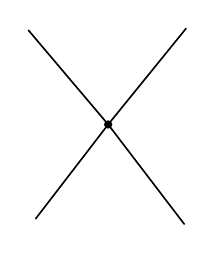
\begin{tikzpicture}[x=.23mm,y=-.23mm,line cap=round]
\draw[line width=.59pt] (16,14)--(60,66)--(102,121)
      (103,13)--(60,66)--(20,118);
\fill (60,66) circle (1.5pt);
\end{tikzpicture}}\endgroup}
\end{GelfandAdjacentEvidence}
\begin{GelfandAdjacentEvidence}{GELFAND-P000465}{9}

— будет беск. число.

\SourceFigure{GELFAND-P000465}{forbidden-forks}{На обоих концах цепочки развилки. Пять узлов обозначены на самой цепочке.
\par\smallskip\centering\color{black}
\begingroup\color{black}\GelfandFitDiagram{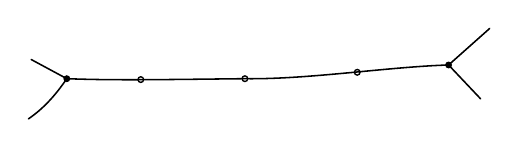
\begin{tikzpicture}[x=.116mm,y=-.116mm,line cap=round]
\draw[line width=.56pt] (18,51)--(57,72)
 .. controls (109,74) and (161,73) .. (252,72)
 .. controls (321,73) and (409,59) .. (475,57)
 -- (520,17);
\draw[line width=.56pt] (57,72)..controls(44,91)and(31,105)..(15,116)
   (475,57)--(510,94);
\fill (57,72) circle (1.25pt) (475,57) circle (1.25pt);
\foreach \x/\y in {138/73,252/72,375/65}{\draw[line width=.5pt] (\x,\y) circle (1.02pt);}
\end{tikzpicture}}\endgroup}
\end{GelfandAdjacentEvidence}
\begin{GelfandAdjacentEvidence}{GELFAND-P000465}{10}

— тоже невозм., т.к. отожд.
\Unclear{GELFAND-P000465}{fork-explanation}{Последнее сокращение предположительно «отожд.».}
\end{GelfandAdjacentEvidence}
\begin{GelfandAdjacentEvidence}{GELFAND-P000465}{11}


$2)$\quad \uwave{Кол-во неразл. об. не зависит от напр. стрелок.}

\uwave{Он характериз. набором размерностей}!!

надо рассм. сист. корней

$\gamma$ — полож. корень,\qquad $\alpha_i$ — пр. корни.

Каждому корню — неразл. объект
\[
\gamma=\sum n_i\alpha_i,\qquad n_i\text{ — размерности!!}
\]
\Unclear{GELFAND-P000465}{root-symbol}{Оба знака имеют нижнюю петлю и два верхних штриха. Условно набрано $\gamma$.}
\end{GelfandAdjacentEvidence}
\begin{GelfandAdjacentEvidence}{GELFAND-P000465}{12}


Кол-во $=$ кол-ву простых корней.
\Unclear{GELFAND-P000465}{root-count}{В этой строке читается «простых корней».}
\end{GelfandAdjacentEvidence}
\begin{GelfandAdjacentEvidence}{GELFAND-P000465}{13}


\SourceFigure{GELFAND-P000465}{a3-example}{Под цепочкой с двумя стрелками вправо стоят шесть строк размерностей.
\par\smallskip\centering\color{black}
\begingroup\color{black}\GelfandFitDiagram{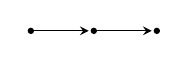
\begin{tikzpicture}[x=1mm,y=1mm,>=stealth,line cap=round]
\fill (0,0) circle (1.15pt) (8,0) circle (1.15pt) (16,0) circle (1.15pt);
\draw[->,shorten >=.65mm] (0,0)--(8,0);
\draw[->,shorten >=.65mm] (8,0)--(16,0);
\end{tikzpicture}}\endgroup\par\smallskip
$\begin{array}{ccc}
1&0&0\\
0&1&0\\
0&0&1\\
1&1&0\\
0&1&1\\
1&1&1
\end{array}$}
\end{GelfandAdjacentEvidence}
\begin{GelfandAdjacentEvidence}{GELFAND-P000465}{14}

\Unclear{GELFAND-P000465}{array-overwrite}{Средняя единица во второй строке наведена. Справа от неё виден остаток петли.}
\end{GelfandAdjacentEvidence}



\Needspace{7\baselineskip}
\begin{GelfandAdjacentEvidence}{GELFAND-P000466}{1}
\SourcePage{GELFAND-P000466}{unlabelled}
$3)$\quad \uwave{Рассм. те \mbox{$\Gamma$}, для к-рых \mbox{$\operatorname{Cat}(\Gamma)$} разрешима.}

\SourceFigure{GELFAND-P000466}{loop-category}{Две петли имеют общий узел. В верхней петле есть короткий косой штрих, отдельно от наконечника.
\par\smallskip\centering\color{black}
\begingroup\color{black}\GelfandFitDiagram{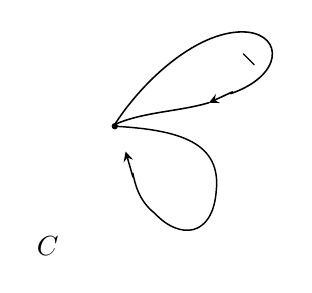
\begin{tikzpicture}[x=.23mm,y=-.23mm,line cap=round,line join=round,>=stealth]
\fill (72,63) circle (1.15pt);
\draw[line width=.56pt] (72,62)
  .. controls (88,37) and (119,9) .. (145,11)
  .. controls (165,13) and (165,35) .. (136,45);
\draw[->,line width=.57pt] (137,44)--(124,50);
\draw[line width=.56pt] (124,50)..controls(107,55)and(88,55)..(72,62);
\draw[line width=.53pt] (72,63)
  .. controls (108,65) and (131,72) .. (128,99)
  .. controls (126,124) and (108,126) .. (94,111)
  .. controls (85,104) and (83,94) .. (82,89);
\draw[->,line width=.55pt] (82,91)--(78,77);
\draw[line width=.42pt] (143,23)--(149,29);
\node at (35,129) {$C$};
\end{tikzpicture}}\endgroup}
\end{GelfandAdjacentEvidence}
\begin{GelfandAdjacentEvidence}{GELFAND-P000466}{2}


Неразрешим. катег. — если есть влож. $C\longrightarrow\operatorname{Cat}(\Gamma)$,
перев. неизом. объекты в неизом.

Они классиф. и соотв. расшир. схемам Дынкина!

\SourceFigure{GELFAND-P000466}{three-arrow}{Три стрелки выходят из одного узла вверх, вправо и влево вниз.
\par\smallskip\centering\color{black}
\begingroup\color{black}\GelfandFitDiagram{\begin{tikzpicture}[x=.22mm,y=-.22mm,line cap=round,>=stealth]
\fill (83,101) circle (1.2pt);
\draw[->,line width=.62pt] (83,101)--(83,21);
\draw[->,line width=.59pt] (83,101)..controls(116,94)and(158,97)..(204,93);
\draw[->,line width=.6pt] (83,101)--(24,171);
\end{tikzpicture}}\endgroup}
\end{GelfandAdjacentEvidence}
\begin{GelfandAdjacentEvidence}{GELFAND-P000466}{3}


\SourceFigure{GELFAND-P000466}{affine-a}{Семь точек соединены вдоль прямой. Дуга соединяет крайние точки.
\par\smallskip\centering\color{black}
\begingroup\color{black}\GelfandFitDiagram{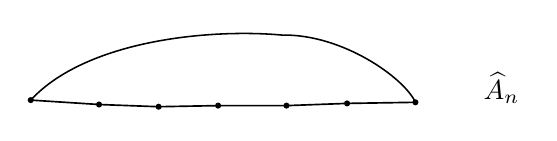
\begin{tikzpicture}[x=.14mm,y=-.14mm,line cap=round]
\draw[line width=.6pt] (22,82)--(84,86)--(138,88)--(192,87)--(254,87)--(309,85)--(371,84);
\draw[line width=.56pt] (22,82)..controls(72,28)and(183,17)..(250,23)
  ..controls(305,22)and(361,62)..(371,84);
\foreach \x/\y in {22/82,84/86,138/88,192/87,254/87,309/85,371/84}
 {\fill (\x,\y) circle (1.1pt);}
\node at (449,71) {$\widehat A_n$};
\end{tikzpicture}}\endgroup}
\end{GelfandAdjacentEvidence}
\begin{GelfandAdjacentEvidence}{GELFAND-P000466}{4}


\SourceFigure{GELFAND-P000466}{affine-d}{Семь точек вдоль цепочки и две ветви на каждом конце.
\par\smallskip\centering\color{black}
\begingroup\color{black}\GelfandFitDiagram{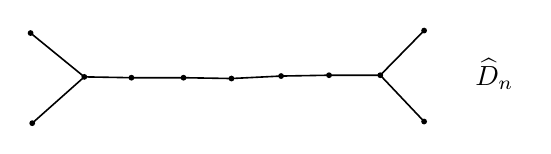
\begin{tikzpicture}[x=.105mm,y=-.105mm,line cap=round]
\draw[line width=.58pt] (24,23)--(89,76)--(146,77)--(209,77)--(267,78)--(327,75)--(385,74)--(447,74)--(500,20);
\draw[line width=.58pt] (26,132)--(89,76) (447,74)--(500,130);
\foreach \x/\y in {24/23,26/132,89/76,146/77,209/77,267/78,327/75,385/74,447/74,500/20,500/130}
 {\fill (\x,\y) circle (1.05pt);}
\node at (585,73) {$\widehat D_n$};
\end{tikzpicture}}\endgroup}
\end{GelfandAdjacentEvidence}
\begin{GelfandAdjacentEvidence}{GELFAND-P000466}{5}


\SourceFigure{GELFAND-P000466}{affine-e}{Семь точек на горизонтали. От третьей слева отходят вниз два отрезка с точками.
\par\smallskip\centering\color{black}
\begingroup\color{black}\GelfandFitDiagram{\begin{tikzpicture}[x=.118mm,y=-.118mm,line cap=round]
\draw[line width=.57pt] (35,77)--(83,76)--(147,73)--(204,72)--(262,72)--(325,71)--(376,73);
\draw[line width=.57pt] (147,73)--(150,134)--(151,185);
\foreach \x/\y in {35/77,83/76,147/73,204/72,262/72,325/71,376/73,150/134,151/185}
 {\fill (\x,\y) circle (1.08pt);}
\node at (500,72) {$\widehat E_n$};
\end{tikzpicture}}\endgroup}
\end{GelfandAdjacentEvidence}
\begin{GelfandAdjacentEvidence}{GELFAND-P000466}{6}


(появл. в теории \(\overset{\text{\sout{гр.}}}{\vphantom{x}}\) групп, порождённых отражениями.)
\Unclear{GELFAND-P000466}{cancel-in-group-comment}{Зачёркнутая приписка над строкой предположительно «гр».}
\end{GelfandAdjacentEvidence}
\begin{GelfandAdjacentEvidence}{GELFAND-P000466}{7}


Это все графы, для к-рых зад. разрешима.

\uuline{В. Бухштабер.}

\uuline{Теор. Лазура.}
\Unclear{GELFAND-P000466}{theorem-name}{Фамилия здесь предположительно «Лазура». Возможное чтение гласной — «а».}
\end{GelfandAdjacentEvidence}
\begin{GelfandAdjacentEvidence}{GELFAND-P000466}{8}

\[
\Lambda=\mathbb Z[a_1,\ldots,a_n,\ldots],\qquad\deg a_n=n\ge1.
\]
\underline{Док-во.}
\[
\Lambda\longrightarrow\bar\Lambda=\Lambda/(\text{разл.})
\]
\Unclear{GELFAND-P000466}{decomposables-quotient}{Над второй $\Lambda$ горизонтальная черта. В знаменателе читается «разл.».}
\end{GelfandAdjacentEvidence}
\begin{GelfandAdjacentEvidence}{GELFAND-P000466}{9}


$\bar\Lambda$ — \uwave{универс. кольцо для}
\(\underset{\downarrow}{\boxed{\text{\scriptsize таких}}}\)
\uwave{полиномов} $h(x,y)$,
\SourceFigure{GELFAND-P000466}{such-insertion}{«таких» вписано в выноску перед «полиномов».}
\end{GelfandAdjacentEvidence}
\begin{GelfandAdjacentEvidence}{GELFAND-P000466}{10}


\(\underset{\downarrow}{\boxed{\text{\scriptsize что}}}\)\quad
$h(x,y)=h(y,x)$,\quad $h(x,0)=0$,
\[
h(y,z)+h(x,y+z)=h(x,z)+h(y,x+z).
\]
\SourceFigure{GELFAND-P000466}{that-insertion}{«что» вписано в отдельную выноску перед условиями.}
\end{GelfandAdjacentEvidence}
\begin{GelfandAdjacentEvidence}{GELFAND-P000466}{11}


Это когомологии:\quad $\underset{\text{(циклы)}}{dh}=0$
\qquad (в бар-конструкции для полиномов)
\Unclear{GELFAND-P000466}{cycle-caption}{Под $dh$ читается «циклы».}
\end{GelfandAdjacentEvidence}
\begin{GelfandAdjacentEvidence}{GELFAND-P000466}{12}


\[
\operatorname{Ext}^{*,*}_{A[x]}(A,A)=H^{*,*}(A[x])
\]
\Unclear{GELFAND-P000466}{cohomology-conventions}{Под $\operatorname{Ext}$ стоит $A[x]$. В обеих частях сверху по две звёздочки.}
\end{GelfandAdjacentEvidence}
\begin{GelfandAdjacentEvidence}{GELFAND-P000466}{13}

\[
\begin{gathered}
A[x]\longrightarrow A[x]\otimes\bar A[y]\\
x\longrightarrow x+y
\end{gathered}
\]
\Unclear{GELFAND-P000466}{normalized-coproduct}{Под первой стрелкой написано $x\longrightarrow x+y$.}
\end{GelfandAdjacentEvidence}
\begin{GelfandAdjacentEvidence}{GELFAND-P000466}{14}


Когом. счит. с пом. резольвент.

Бар-констр. — одна из резольвент.

\[
\mathcal A:\quad
A[x]\xrightarrow{\Delta}A[x]\otimes\bar A[y]
\longrightarrow A[x]\otimes\bar A[y]\otimes\bar A[z]\longrightarrow\ldots
\]
$\bar A[y]$ — многочлены без своб. члена.

Получ. ацикличный комплекс, к-рый прим. для вычисл. когомологий
\[
(\text{ставим }\underset{h(x,y)}{\text{всюду}}\text{ — }
\tilde a\Rightarrow a\otimes1+1\otimes a)=\Delta a).
\]
\Unclear{GELFAND-P000466}{primitive-condition}{Над $a$ волнистая черта. Следующий знак предположительно $\Rightarrow$. Видны обе закрывающие скобки.}
\end{GelfandAdjacentEvidence}
\begin{GelfandAdjacentEvidence}{GELFAND-P000466}{15}


Надо классиф. циклы в конкретной резольвенте.
\[
0\longrightarrow B\longrightarrow Z\longrightarrow H^2(A[x])\longrightarrow0
\]
\Unclear{GELFAND-P000466}{exact-sequence}{После $B$ написано $Z$, у $H$ верхний индекс $2$.}
\end{GelfandAdjacentEvidence}


$x^n\longrightarrow(x+y)^n-x^n-y^n$\qquad (это границы)


\Needspace{7\baselineskip}
\begin{GelfandAdjacentEvidence}{GELFAND-P000467}{1}
\SourcePage{GELFAND-P000467}{unlabelled}
Переход к полученн. резольв. с пом. функтора $\operatorname{Hom}(\cdot,A)$
\Unclear{GELFAND-P000467}{opening-word}{Сокращение перед «резольв.» читается «полученн.».}
\end{GelfandAdjacentEvidence}
\begin{GelfandAdjacentEvidence}{GELFAND-P000467}{2}


В ацикл. резольв.
\[
\begin{aligned}
x&\longrightarrow x+y\\
x^n&\longrightarrow(x+y)^n.
\end{aligned}
\]
Надо рассм. $\operatorname{Hom}_{A[x]}(\mathcal A,A)$
(по $1$-му сомножителю уст. структ. $A[x]$-мод.).
\Unclear{GELFAND-P000467}{hom-module-conventions}{У $\operatorname{Hom}$ нижний индекс $A[x]$. В скобках $\mathcal A,A$.}
\end{GelfandAdjacentEvidence}
\begin{GelfandAdjacentEvidence}{GELFAND-P000467}{3}

\Unclear{GELFAND-P000467}{parenthetical-abbreviation}{После «сомножителю» читается «уст.».}
\end{GelfandAdjacentEvidence}
\begin{GelfandAdjacentEvidence}{GELFAND-P000467}{4}


\[
A\xrightarrow{d} A[y]\xrightarrow{d} A[y]\otimes A[z]\xrightarrow{d}\ldots
\]
\Unclear{GELFAND-P000467}{cochain-conventions}{На этой строке $A[y]$ и $A[z]$ записаны без надчёркиваний.}
\end{GelfandAdjacentEvidence}
\begin{GelfandAdjacentEvidence}{GELFAND-P000467}{5}

\[
\Delta\longrightarrow d:\qquad x^n\longrightarrow(x+y)^n-x^n-y^n
\]
\Unclear{GELFAND-P000467}{cochain-boundary-map}{На следующей строке видны оба вычитаемых члена, $x^n$ и $y^n$.}
\end{GelfandAdjacentEvidence}
\begin{GelfandAdjacentEvidence}{GELFAND-P000467}{6}

\[
\Delta:\quad h(x,y)\longrightarrow
h\bigl(\underset{\substack{\Vert\\x+z}}{\Delta x},y\bigr)
-
h\bigl(x,\underset{\substack{\Vert\\y+z}}{\Delta y}\bigr)
\]
\Unclear{GELFAND-P000467}{cochain-sign}{Между членами стоит густо наведённый горизонтальный знак. Условно набран минус.}
\end{GelfandAdjacentEvidence}
\begin{GelfandAdjacentEvidence}{GELFAND-P000467}{7}


$\mathcal A$ — послед. $A[x]$-модулей,
\Unclear{GELFAND-P000467}{module-ending-punctuation}{В конце строки виден низкий короткий штрих, похожий на запятую.}
\end{GelfandAdjacentEvidence}
\begin{GelfandAdjacentEvidence}{GELFAND-P000467}{8}


$A[x]\otimes y^k$ — \uwave{подмодули}

Из-за $\overline{A[y]}$:
\[
x^n\longrightarrow (x+y)^n-x^n\qquad\text{(т.к. без своб. члена)}
\]
\begin{center}
\rule[.5ex]{26mm}{.35pt}\enspace$\bullet$\enspace\rule[.5ex]{25mm}{.35pt}
\end{center}

\SourceFigure{GELFAND-P000467}{right-margin-line}{По правому краю кадра видна длинная черта. Она начинается небольшим загибом и заканчивается немного ниже разделителя.
\par\smallskip\raggedleft\color{black}
\begingroup\color{black}\GelfandFitDiagram{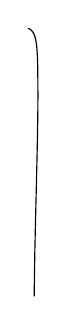
\begin{tikzpicture}[x=1mm,y=1mm,line cap=round]
\draw[line width=.42pt] (0,34)..controls(1.1,33.6)and(1.2,31.8)..(1.22,27)
  ..controls(1.3,21)and(.8,8)..(.76,0);
\end{tikzpicture}}\endgroup}
\end{GelfandAdjacentEvidence}



\Needspace{7\baselineskip}
\begin{GelfandAdjacentEvidence}{GELFAND-P000468}{1}
\SourcePage{GELFAND-P000468}{unlabelled}
\underline{13/\mbox{$\overline{\underline{\mathrm{XI}}}$}-72г.}
\quad\underline{Сем. Гельфанда.}

\underline{Л. Вассерштейн.}

\uuline{\mbox{$A$}} — ассоциат. кольцо (не обязательно с $1$).

\uuline{\mbox{$iA$}} — кольцо с формально присоед. единицей.

$iA/A=\mathbb Z$,\quad $A$ — двустор. идеал в $iA$.

$GA$ — мульт. группа кольца.

$GA\subset A$

$(a,b)\longrightarrow a+b+ab$\qquad Это бинарная ассоц. опер.
\[
\Vert\qquad (e+a)(e+b)-e=a+b+ab
\]
\sout{\mbox{$iA$}}\quad \uuline{\mbox{$GA$}} — мн-во обратимых элементов отн. этой операции.
\Unclear{GELFAND-P000468}{initial-cancel}{Короткая зачёркнутая запись перед $GA$ предположительно $iA$.}
\end{GelfandAdjacentEvidence}
\begin{GelfandAdjacentEvidence}{GELFAND-P000468}{2}


\[
a\longrightarrow1+a,\qquad A\longrightarrow1+A
\]
\uwave{гомоморфизм}.\quad
\begin{tabular}[t]{@{}l@{}}
\underline{в обычные}\\
\underline{обрат. элем}.
\end{tabular}

\[
\begin{gathered}
f:A\longrightarrow B\\
f(GA)\subset GB
\end{gathered}
\]
\Unclear{GELFAND-P000468}{image-containment}{Знак перед $GB$ наведён. Условно набрано $\subset$.}
\end{GelfandAdjacentEvidence}
\begin{GelfandAdjacentEvidence}{GELFAND-P000468}{3}


$i,G$ — функторы в кат. колец с $1$ и кат. групп.

\uuline{\mbox{$M_kA$}} — матрицы $k\times k$ с обычным умножением.

\uuline{\mbox{$\widetilde\Omega A$}}$=\{a=(a_{ij})\}$,
в $\forall$ строке и столбце конеч. число элем. $\ne0$,
(это кольцо)

\uuline{\mbox{$MA$}} — подкольцо конечных матриц (конечное число элем. $\ne0$).
(двустор. идеал в $\widetilde\Omega A$).

\uuline{\mbox{$\Omega A$}}$=\widetilde\Omega A/MA$
\Unclear{GELFAND-P000468}{omega-letter}{Буква перед $A$ слева густо наведена. Читается $\Omega$.}
\end{GelfandAdjacentEvidence}
\begin{GelfandAdjacentEvidence}{GELFAND-P000468}{4}


$M,\widetilde\Omega,\Omega$ — функторы.

\[
\underset{\vert}{\text{\uuline{\mbox{$\Theta A$}}}}\subset MA
\]
верхние треугольные $a=(a_{ij})$:\quad $a_{ij}=0$ при $i\le j$ \sout{\ldots}
\SourceFigure{GELFAND-P000468}{theta-link}{Под двойным подчёркиванием $\Theta A$ проведена короткая вертикальная черта.}
\end{GelfandAdjacentEvidence}
\begin{GelfandAdjacentEvidence}{GELFAND-P000468}{5}

\Unclear{GELFAND-P000468}{triangular-convention}{Написано «верхние треугольные» и $a_{ij}=0$ при $i\le j$.}
\end{GelfandAdjacentEvidence}
\begin{GelfandAdjacentEvidence}{GELFAND-P000468}{6}

\Incomplete{GELFAND-P000468}{cancel-inequality}{После неравенства зачёркнуты несколько знаков один под другим.}
\end{GelfandAdjacentEvidence}
\begin{GelfandAdjacentEvidence}{GELFAND-P000468}{7}


\underline{Замечание}. Если $N\xrightarrow{\sim}N$ биекция, то есть отобр. кольца матриц
(\sout{эт} автом.) — перестан. одноврем. строк и столбцов.
\Unclear{GELFAND-P000468}{cancel-auto}{Зачёркнутое сокращение перед «автом.» предположительно «эт».}
\end{GelfandAdjacentEvidence}
\begin{GelfandAdjacentEvidence}{GELFAND-P000468}{8}

(внутр. автом. перестан. строк и столбцов)
\Unclear{GELFAND-P000468}{inner-ambient}{В скобках читается «внутр. автом.».}
\end{GelfandAdjacentEvidence}
\begin{GelfandAdjacentEvidence}{GELFAND-P000468}{9}


Даже если $N\longrightarrow N$ любое отобр., то ему сопост. \underline{эндоморфизм}.
\Unclear{GELFAND-P000468}{next-word}{Первое слово читается «Даже».}
\end{GelfandAdjacentEvidence}
\begin{GelfandAdjacentEvidence}{GELFAND-P000468}{10}

\Unclear{GELFAND-P000468}{arbitrary-reindexing}{Последнее слово подчёркнуто. Читается «эндоморфизм».}
\end{GelfandAdjacentEvidence}
\begin{GelfandAdjacentEvidence}{GELFAND-P000468}{11}


$GMA$ — мульт. группа, $MA$,\quad $GMA\subset MA$.

\uwave{Симплициальная структура в \mbox{$MA$}.}

$X\subset GMA$ наз. симплексом, если левым сдвигом и сопряжением матрицей перестановок его можно перевести в $\Theta A$
\Unclear{GELFAND-P000468}{left-shift-convention}{В рукописи читается «левым сдвигом».}
\end{GelfandAdjacentEvidence}
\begin{GelfandAdjacentEvidence}{GELFAND-P000468}{12}


Заметим, что $G\Theta A=\Theta A$ как множество (они нильпотентны)
\Unclear{GELFAND-P000468}{final-word}{Последние буквы наведены. Слово читается «нильпотентны».}
\end{GelfandAdjacentEvidence}



\Needspace{7\baselineskip}
\begin{GelfandAdjacentEvidence}{GELFAND-P000469}{1}
\SourcePage{GELFAND-P000469}{unlabelled}
\Incomplete{GELFAND-P000469}{top-cancelled}{Зачёркнутый знак перед первой строкой и короткая черта справа от него. Чтение не установлено.}
\end{GelfandAdjacentEvidence}
\begin{GelfandAdjacentEvidence}{GELFAND-P000469}{2}

На самом деле
\SourceFigure{GELFAND-P000469}{inclusion-bracket}{Линия под включением загнута вверх с двух концов.\par\smallskip\centering
\begingroup\color{black}\GelfandFitDiagram{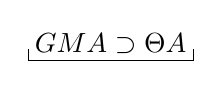
\begin{tikzpicture}
\node[inner sep=2.2pt] (inclusion) at (0,0) {$GMA\supset\Theta A$};
\draw (inclusion.south west) ++(0,4pt) -- (inclusion.south west) -- (inclusion.south east) -- ++(0,4pt);
\end{tikzpicture}}\endgroup}
\end{GelfandAdjacentEvidence}
\begin{GelfandAdjacentEvidence}{GELFAND-P000469}{3}


\uline{Отметим вершину: \mbox{$0$}} — единица группы $GMA$.

\uuline{\mbox{$SA$}} — соответствующая симплициальная схема.

(Историч. замечание: Володин использовал $SA$ для опр. функторов $K_{\mathbb C}^{n}$)
\par по существу
\Unclear{GELFAND-P000469}{top-functor-index}{Нижний индекс читается $\mathbb C$; внутри буквы проведён дополнительный штрих.}
\end{GelfandAdjacentEvidence}
\begin{GelfandAdjacentEvidence}{GELFAND-P000469}{4}


{\centering\rule{2.7em}{.4pt}\quad\textperiodcentered\quad\rule{3.1em}{.4pt}\par}
Пусть в кольце $A$ есть единица. Тогда положим.
\[
K_nA=\pi_{n-1}SA,\qquad n\geqslant1.
\]
При $n\geqslant2$ там есть структура группы, коммутативной при $n\geqslant3$.

\uline{Другое опред. групповой структуры (коммутативной).}

\uline{Лемма Уайтхеда}

Рассм. сфероид $s\colon Z^n\longrightarrow SA$.
На $SA$ действует группа подстановок $f\colon N\longrightarrow N$.
Получ. новый сфероид $s^f$:
\SourceFigure{GELFAND-P000469}{spheroid-diagram}{У верхней стрелки подписи нет.\par\smallskip\centering
\begingroup\color{black}\GelfandFitDiagram{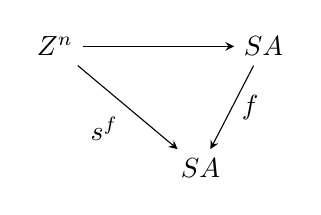
\begin{tikzpicture}[>=stealth]
\node (sphere) at (0,0) {$Z^n$};
\node (top) at (2.65,0) {$SA$};
\node (bottom) at (1.85,-1.55) {$SA$};
\draw[->] (sphere) -- (top);
\draw[->] (sphere) -- node[below left] {$s^f$} (bottom);
\draw[->] (top) -- node[right] {$f$} (bottom);
\end{tikzpicture}}\endgroup}
\end{GelfandAdjacentEvidence}
\begin{GelfandAdjacentEvidence}{GELFAND-P000469}{5}


Они всегда гомотопны.

\uline{Идея док-ва:}

$\operatorname{Im}s\subset M_kA$.
\[
s=\left(\begin{array}{c|c}sz&0\\\hline 0&0\end{array}\right).
\]
Всё сводится к случаю
\[
s^f=\left(\begin{array}{c|c}0&0\\\hline 0&sz\end{array}\right).
\]
\Unclear{GELFAND-P000469}{middle-block-argument}{Последний знак в $sz$ имеет поперечный штрих и условно набран строчной буквой. Обе матрицы имеют две разделительные черты.}
\end{GelfandAdjacentEvidence}
\begin{GelfandAdjacentEvidence}{GELFAND-P000469}{6}


($f$ специального вида: $fi=i+k$, на $\infty$ подправляем).

\[
\begin{pmatrix}a&0\\0&0\end{pmatrix}\quad
\begin{pmatrix}a&a\\0&0\end{pmatrix}\quad
\begin{pmatrix}0&a\\-1&0\end{pmatrix}\quad
\begin{pmatrix}0&0\\-1&a\end{pmatrix}\quad
\begin{pmatrix}0&0\\0&a\end{pmatrix}
\]
\Unclear{GELFAND-P000469}{five-spheroids}{В третьей матрице левый верхний ноль густо наведён.}
\end{GelfandAdjacentEvidence}
\begin{GelfandAdjacentEvidence}{GELFAND-P000469}{7}

Это 5 сфероидов. Это гомотопия. Каждые 2 соседних элементарно гомотопны:

\[
s_1,s_2\colon S'\longrightarrow S'
\]
наз. элем. гомотопными, если $\forall$ симплекса $X\subset S$, $s_1X\cup s_2X$
есть симплекс в $S'$.
\Unclear{GELFAND-P000469}{homotopy-domain}{Над первым $S$ виден короткий штрих. В следующей строке написано $X\subset S$ без штриха.}
\end{GelfandAdjacentEvidence}
\begin{GelfandAdjacentEvidence}{GELFAND-P000469}{8}


Пусть все $a$ лежат в одном симплексе $X$.
Тогда $\begin{pmatrix}a&0\\0&0\end{pmatrix}$ и
$\begin{pmatrix}a&a\\0&0\end{pmatrix}$ лежат в одном симплексе.

Пусть $a_0^{-1}\in X$. Умножим на $a_0$. Тогда они станут верхнетреуг.
Если все $a$ верхне-треугольные, то все 5 матриц лежат в одном симплексе.

{\centering\rule{3em}{.4pt}\quad\textperiodcentered\quad\rule{3.5em}{.4pt}\par}
\uline{Структура коммут. группы в \mbox{$K_nA$}.}
\[
MA\times MA\xrightarrow{\oplus}MA
\]
\[
\begin{array}{@{}ll|l@{}}
fi=2i & f,g\colon\mathbb N\longrightarrow\mathbb N & \text{некоммут., неассоц., без}\\
gi=2i+1 & a\oplus b=a^f+b^g & \text{нейтр. элем.}
\end{array}
\]
\SourceFigure{GELFAND-P000469}{group-operation-margin}{Запись о свойствах операции отделена вертикальной чертой.}
\end{GelfandAdjacentEvidence}
\begin{GelfandAdjacentEvidence}{GELFAND-P000469}{9}


\Unclear{GELFAND-P000469}{margin-left-bottom}{За левой границей текста видны наклонный штрих и знак, похожий на закрывающую скобку. Их назначение не установлено.}
\end{GelfandAdjacentEvidence}



\Needspace{7\baselineskip}
\begin{GelfandAdjacentEvidence}{GELFAND-P000470}{1}
\SourcePage{GELFAND-P000470}{unlabelled}
она индуцирует отобр. $SA\times SA\longrightarrow SA$,
что даёт операции на всех $K_i$, $i\geqslant0$. (корр. прв. по лемме Уайтхеда)
\Unclear{GELFAND-P000470}{whitehead-abbreviation}{Второе сокращение после «корр.» условно читается «прв.».}
\end{GelfandAdjacentEvidence}
\begin{GelfandAdjacentEvidence}{GELFAND-P000470}{2}

Они коммутативны и совпад. с ранее введёнными в силу взаимной дистрибутивности, проверяемой по лемме Уайтхеда.

{\centering\rule{2em}{.4pt}\quad\textperiodcentered\quad\rule{3.4em}{.4pt}\par}
Можно определить сумму — $H$-пр-во.
На $\widetilde\Omega A$ склад. даже беск. число матриц!
Отсюда оно будет иметь тривиальные $K$-функторы.
\Unclear{GELFAND-P000470}{omega-mark}{У $\Omega$ сверху длинный волнистый знак. Набрано $\widetilde\Omega$.}
\end{GelfandAdjacentEvidence}
\begin{GelfandAdjacentEvidence}{GELFAND-P000470}{3}


{\centering\rule{2.4em}{.4pt}\quad\textperiodcentered\quad\rule{3.1em}{.4pt}\par}
\uuline{\mbox{$K_1A=\pi_0SA$}.}

Это мн-во компон. связности в $GMA$.

$EA$ — связная компон. единицы. (произведения \(\underset{\substack{\vert\\\text{\scriptsize псевдотреугольные}}}{\text{элем.}}\) матриц),
\SourceFigure{GELFAND-P000470}{pseudo-triangular-insertion}{Под «элем.» написано «псевдотреугольные», с соединительным штрихом.}
\end{GelfandAdjacentEvidence}
\begin{GelfandAdjacentEvidence}{GELFAND-P000470}{4}


\SourceFigure{GELFAND-P000470}{perfectness-hypotheses}{Ступенчатый контур охватывает оба условия; стрелка начинается на уровне первого.\par\smallskip\centering
\begingroup\color{black}\GelfandFitDiagram{\begin{tikzpicture}[inner sep=3pt]
\node[anchor=west] (unit) at (0,0) {$A\ni1$};
\node[anchor=west] (alt) at (0,-.56) {или};
\node[anchor=west] (idem) at (0,-1.12) {$AA=A$ (в кольцевом умн.)};
\draw (unit.north west) -- (unit.north east) |- (alt.north east -| idem.east)
      -- (idem.south east) -- (idem.south west) -- cycle;
\node[right] at (unit.east) {$\Longrightarrow$};
\end{tikzpicture}}\endgroup}
\end{GelfandAdjacentEvidence}
\begin{GelfandAdjacentEvidence}{GELFAND-P000470}{5}

\[
EA=[GMA,GMA]=[EA,EA].
\]

$K_2A$ — гомот. классы петель. Петли — соотношения элем. матриц.

$\Theta A$ имеет образующие $a^{ij}$
\Incomplete{GELFAND-P000470}{middle-generator-cancelled}{После $a^{ij}$ запись густо зачёркнута. Под словом «Петли» видна короткая стрелка влево.}
\end{GelfandAdjacentEvidence}
\begin{GelfandAdjacentEvidence}{GELFAND-P000470}{6}

(на $i,j$ -м месте стоит $a\in A$).

Соотнош.: Стейнберга
\[
\begin{gathered}
a^{ij}\ast b^{ij}=(a+b)^{ij},\\
[a^{ij},b^{jk}]=(ab)^{ik}
\end{gathered}
\]
и у нек-рых коммутатор $0$.

Это определяющие соотношения.

Пусть $StA$ — группа, порожд. этими образ. и соотн.
\[
0\longrightarrow K_2A\longrightarrow StA\longrightarrow EA\longrightarrow0
\]
\[
\begin{gathered}
\vert\\[-.2ex]
\text{гомот. классы путей из }0\text{ куда-то}\\
\text{(с фикс. нач. и концом)}
\end{gathered}
\]
\SourceFigure{GELFAND-P000470}{steinberg-paths}{Пояснение соединено вертикальным штрихом с $StA$.}
\end{GelfandAdjacentEvidence}
\begin{GelfandAdjacentEvidence}{GELFAND-P000470}{7}


{\centering\rule{3.1em}{.4pt}\quad\textperiodcentered\quad\rule{4em}{.4pt}\par}
\Unclear{GELFAND-P000470}{lower-margin-mark}{Слева от формулы одиночный наведённый знак. Чтение не установлено.}
\end{GelfandAdjacentEvidence}
\begin{GelfandAdjacentEvidence}{GELFAND-P000470}{8}

\[
K_2A=\underset{\text{(гомологии группы)}}{\underbrace{H_2EA}}\qquad\sim\qquad
StA=\text{универс. центр. расширение }EA.
\]

\uline{Задача:} пусть есть 3 матрицы в $GMA$. Все отрезки — симплекс.
Тогда все 3 — симплекс.

Обобщение: если любая пара симплекс, то все симплекс.
(пр-во \uline{толерантности})

{\centering\rule{4em}{.4pt}\quad\textperiodcentered\quad\rule{2.3em}{.4pt}\par}
\uuline{Д. А. Каждан.}\qquad\uline{Производная категория.}

$C$ — абелева категория. Рассм. категорию комплексов $K_C$.
\SourceFigure{GELFAND-P000470}{complexes-diagram}{В обоих столбцах стрелки направлены вверх. Между столбцами две стрелки вправо.\par\smallskip\centering
\begingroup\color{black}\GelfandFitDiagram{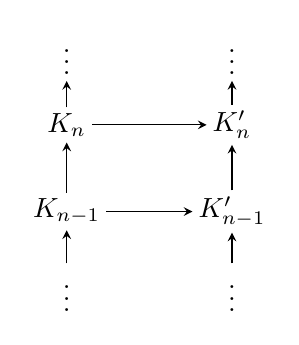
\begin{tikzpicture}[>=stealth,every node/.style={inner sep=2pt}]
\node (l0) at (0,0) {$\vdots$}; \node (r0) at (2.1,0) {$\vdots$};
\node (l1) at (0,-.9) {$K_n$}; \node (r1) at (2.1,-.9) {$K'_n$};
\node (l2) at (0,-2) {$K_{n-1}$}; \node (r2) at (2.1,-2) {$K'_{n-1}$};
\node (l3) at (0,-3) {$\vdots$}; \node (r3) at (2.1,-3) {$\vdots$};
\draw[->] (l1) -- (r1);
\draw[->] (l2) -- (r2);
\draw[->] (l1) -- (l0);
\draw[->] (l2) -- (l1);
\draw[->] (l3) -- (l2);
\draw[->] (r1) -- (r0);
\draw[->] (r2) -- (r1);
\draw[->] (r3) -- (r2);
\end{tikzpicture}}\endgroup}
\end{GelfandAdjacentEvidence}
\begin{GelfandAdjacentEvidence}{GELFAND-P000470}{9}


\Unclear{GELFAND-P000470}{bottom-cancelled-words}{Перед «морфизмами» зачёркнут фрагмент. Возможно «с сост. об.».}
\end{GelfandAdjacentEvidence}
\begin{GelfandAdjacentEvidence}{GELFAND-P000470}{10}

\uline{морфизмами \mbox{$f$} гомот. классами морфизмов комплексов.}
\Unclear{GELFAND-P000470}{bottom-right-cancelled}{После «морфизмов» зачёркнут одиночный знак, чтение не установлено.}
\end{GelfandAdjacentEvidence}
\begin{GelfandAdjacentEvidence}{GELFAND-P000470}{11}

\SourceFigure{GELFAND-P000470}{morphism-underline}{Под двумя строками проведено непрерывное ступенчатое подчёркивание.}
\end{GelfandAdjacentEvidence}
\begin{GelfandAdjacentEvidence}{GELFAND-P000470}{12}


\[
\begin{gathered}
S\subset\operatorname{Hom}K_C\\[-.2ex]
\vert\\[-.2ex]
\text{морф., индуц. изоморфизм гомологий}
\end{gathered}
\]
\SourceFigure{GELFAND-P000470}{homology-label}{Пояснение соединено вертикальным штрихом с $S$.}
\end{GelfandAdjacentEvidence}



\Needspace{7\baselineskip}
\begin{GelfandAdjacentEvidence}{GELFAND-P000471}{1}
\SourcePage{GELFAND-P000471}{unlabelled}
\uline{Лемма}. Пусть $f;g\colon K\longrightarrow K'$ два морфизма.
\Unclear{GELFAND-P000471}{lemma-delimiter}{Между $f$ и $g$ видны два штриха; набрана точка с запятой.}
\end{GelfandAdjacentEvidence}
\begin{GelfandAdjacentEvidence}{GELFAND-P000471}{2}


След. утв. эквивалентны:

$1^\circ$. $\exists K_1$, $s_1\in S$:
\SourceFigure{GELFAND-P000471}{lemma-precomposition}{Схема первого условия и равенство под ней.\par\smallskip\centering
\begingroup\color{black}\GelfandFitDiagram{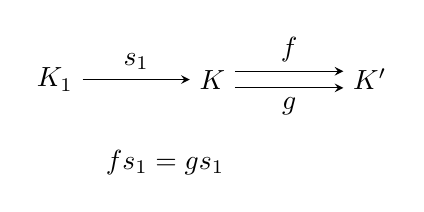
\begin{tikzpicture}[>=stealth]
\node (start) at (0,0) {$K_1$};
\node (middle) at (2,0) {$K$};
\node (end) at (4,0) {$K'$};
\draw[->] (start) -- node[above] {$s_1$} (middle);
\draw[->] ([yshift=3pt]middle.east) -- node[above] {$f$} ([yshift=3pt]end.west);
\draw[->] ([yshift=-3pt]middle.east) -- node[below] {$g$} ([yshift=-3pt]end.west);
\node at (1.4,-1.05) {$fs_1=gs_1$};
\end{tikzpicture}}\endgroup}
\end{GelfandAdjacentEvidence}
\begin{GelfandAdjacentEvidence}{GELFAND-P000471}{3}


$2^\circ$. $\exists K_2$, $s_2\in S$
\SourceFigure{GELFAND-P000471}{lemma-postcomposition}{Схема второго условия и равенство под ней.\par\smallskip\centering
\begingroup\color{black}\GelfandFitDiagram{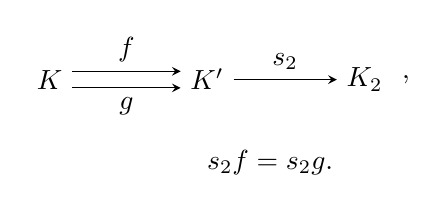
\begin{tikzpicture}[>=stealth]
\node (start) at (0,0) {$K$};
\node (middle) at (2,0) {$K'$};
\node (end) at (4,0) {$K_2$};
\draw[->] ([yshift=3pt]start.east) -- node[above] {$f$} ([yshift=3pt]middle.west);
\draw[->] ([yshift=-3pt]start.east) -- node[below] {$g$} ([yshift=-3pt]middle.west);
\draw[->] (middle) -- node[above] {$s_2$} (end);
\node[right] at (end.east) {,};
\node at (2.8,-1.05) {$s_2f=s_2g$.};
\end{tikzpicture}}\endgroup}
\end{GelfandAdjacentEvidence}
\begin{GelfandAdjacentEvidence}{GELFAND-P000471}{4}


{\centering\rule{3em}{.4pt}\quad\textperiodcentered\quad\rule{3.4em}{.4pt}\par}
$L_C$ — те же объекты, а морфизмы: \uline{разреш. обращать \mbox{$s^{-1}$} и}
\par\hspace*{3em}\uline{соотношения Оре.}
\SourceFigure{GELFAND-P000471}{ore-insertion}{«соотношения Оре» написано ниже, под ступенчатой чертой.}
\end{GelfandAdjacentEvidence}
\begin{GelfandAdjacentEvidence}{GELFAND-P000471}{5}

Лемма даёт возможно корректно опр. произведение.
\Unclear{GELFAND-P000471}{product-reading}{Перед «корректно» читается «возможно».}
\end{GelfandAdjacentEvidence}
\begin{GelfandAdjacentEvidence}{GELFAND-P000471}{6}


{\centering\rule{3em}{.4pt}\quad\textperiodcentered\quad\rule{3.5em}{.4pt}\par}
\(\overset{\scriptstyle +}{\text{См.}}\)\quad\uline{Hartshorne}. Residues and duality.
\Unclear{GELFAND-P000471}{middle-reference-mark}{Над «См.» стоит короткая крестообразная помета.}
\end{GelfandAdjacentEvidence}
\begin{GelfandAdjacentEvidence}{GELFAND-P000471}{7}


{\centering\rule{3.9em}{.4pt}\quad\textperiodcentered\quad\rule{3.4em}{.4pt}\par}
\uuline{В. Бухштабер.}

\begin{tabular}{@{}llll@{}}
Ссылки: & К.-Э. & 213--223 & (Картан и Эйленберг)\\
 & М. & 358--370 & (Маклейн)\\
 & Адамс & Мат. $3\colon4$ & стр. 7--19.
\end{tabular}
\Unclear{GELFAND-P000471}{middle-maclane}{В скобках читается «Маклейн».}
\end{GelfandAdjacentEvidence}
\begin{GelfandAdjacentEvidence}{GELFAND-P000471}{8}


{\centering\rule{2.8em}{.4pt}\quad\textperiodcentered\quad\rule{3em}{.4pt}\par}
\[
A=\sum_{n\geqslant0}A_n\qquad\text{— градуир. кольцо.}
\]
$A_n$ — $A_0$-модуль для любого $n\geqslant0$.
\[
0\longleftarrow A_0\xleftarrow{\varepsilon}A
\longleftarrow C_1\longleftarrow C_2\longleftarrow\cdots
\longleftarrow C_s\xleftarrow{d_{s+1}}C_{s+1}\longleftarrow\cdots
\]
($\varepsilon$ сопост. $A$ нулев. компон. каждому $a\in A$).
\Unclear{GELFAND-P000471}{lower-augmentation-a}{Отдельная буква $A$ написана сразу после «сопост.».}
\end{GelfandAdjacentEvidence}
\begin{GelfandAdjacentEvidence}{GELFAND-P000471}{9}


Доп. до \uwave{градуир. своб. резольвенты}.

Функтор $\operatorname{Hom}_A(\cdot,A_0)$. переводит $d_s$ в $(d_s)^*$.
\Unclear{GELFAND-P000471}{lower-hom-coefficient}{У второго аргумента $A$ внизу справа виден маленький ноль, вплотную к скобке.}
\end{GelfandAdjacentEvidence}
\begin{GelfandAdjacentEvidence}{GELFAND-P000471}{10}

\[
H^s(A)=\operatorname{Ker}(d_{s+1})^*/\operatorname{Im}(d_s)^*
\]
\SourceFigure{GELFAND-P000471}{cohomology-index}{В числителе $d_{s+1}$, в знаменателе $d_s$.}
\end{GelfandAdjacentEvidence}


\uline{Теорема:}\quad 1) Сущ. своб. резольвента

\hspace*{6em}2) Группы $H^s(A)$ не зависят от резольвенты.

\[
H(A)=\sum_{s=0}^{\infty}H^s(A)\qquad\text{— градуированное кольцо.}
\]
Будет дано опр. умн. \uline{Йонеда}.
\[
\begin{gathered}
f\in H^i(A),\quad g\in H^j(A),\quad fg\in H^{i+j}(A),\\
\widetilde f\colon C_i\longrightarrow A_0;\qquad
\widetilde g\colon C_j\longrightarrow A_0.
\end{gathered}
\]


\Needspace{7\baselineskip}
\begin{GelfandAdjacentEvidence}{GELFAND-P000472}{1}
\SourcePage{GELFAND-P000472}{unlabelled}
\SourceFigure{GELFAND-P000472}{top-product-diagram}{Узел $C_1$ густо наведён. От $C_i$ к $A$ идёт прерывистая стрелка, у стрелки от $C_{i+j}$ к $C_j$ один разрыв.\par\smallskip\centering
\begingroup\color{black}\GelfandFitDiagram{\begin{tikzpicture}[>=stealth]
\node (ci) at (1.5,1.8) {$C_i$};
\node (topdots) at (3.15,1.8) {$\cdots$};
\node at (5.1,1.8) {$\cdots$};
\node (cij) at (6.7,1.8) {$C_{i+j}$};
\node (a0) at (0,0) {$A_0$};
\node (a) at (1.5,0) {$A$};
\node (c1) at (3.1,0) {$C_1$};
\node (dots) at (4.65,0) {$\cdots$};
\node (cj) at (6.1,0) {$C_j$};
\node (out) at (6.1,-1.5) {$A_0$};
\draw[->] (topdots) -- (ci);
\draw[->] (cj) -- (dots);
\draw[->] (dots) -- (c1);
\draw[->] (c1) -- (a);
\draw[->] (a) -- (a0);
\draw[->] (ci) -- node[left] {$\widetilde f$} (a0);
\draw[->,densely dashed] (ci) -- (a);
\draw (cij.south) -- (6.44,1.03);
\draw[->] (6.38,.91) -- (cj.north);
\draw[->] (cj) -- node[left] {$\widetilde g$} (out);
\end{tikzpicture}}\endgroup}
\end{GelfandAdjacentEvidence}
\begin{GelfandAdjacentEvidence}{GELFAND-P000472}{2}


Получили гомоморфизм $C_{i+j}\longrightarrow A_0$.
\Unclear{GELFAND-P000472}{homomorphism-verb}{Первое слово читается «Получили», предпоследняя буква сближена с последней.}
\end{GelfandAdjacentEvidence}
\begin{GelfandAdjacentEvidence}{GELFAND-P000472}{3}


Получится
\[
A\underset{\text{сопост.}}{\rightsquigarrow}H(A)
\qquad\text{(кольцо)}
\]
$H(A)$ вообще говоря некоммутативно (!) по настоящему.
На этом основана классифик. многозн. групп.
\Unclear{GELFAND-P000472}{multivalued-groups}{После «классифик.» читается «многозн.».}
\end{GelfandAdjacentEvidence}
\begin{GelfandAdjacentEvidence}{GELFAND-P000472}{4}

(В топологии до сих пор встр. только коммут. кольца — там всегда алгебры Хопфа).

\uline{Станд. резольвента или \mbox{$B$}-резольвента.}
\[
\overline A=\sum_{n>0}A_n
\]
\[
C_1=A\underset{A_0}{\otimes}\overline A
\qquad\text{В дальнейшем }A_0\text{ опускается}
\]
(Исх. кольца коммутативны!)
\[
\begin{gathered}
C_s=A\otimes(\overline A)^s.\\
d_{s+1}\colon A\otimes(\overline A)^{s+1}
\longrightarrow A\otimes(\overline A)^s
\end{gathered}
\]
\[
\begin{aligned}
d_s\bigl(a_0[a_1|a_2|\ldots|a_s]\bigr)
={}&(-1)^{\varepsilon(0)}a_0a_1[a_2|\ldots a_s]\\
 &+\sum(-1)^{\varepsilon(n)}a_0[a_1|\ldots|a_na_{n+1}|\ldots a_s]
\end{aligned}
\]
\Unclear{GELFAND-P000472}{bar-differential-indices}{Два индекса в произведении наведены. Читается $a_na_{n+1}$.}
\end{GelfandAdjacentEvidence}
\begin{GelfandAdjacentEvidence}{GELFAND-P000472}{5}


$\varepsilon(n)$ — некоторые ф-ии от номера,
\sout{Для чётной градуир. \mbox{$\varepsilon(n)=n$}.}
\par\uline{\mbox{$\varepsilon(n)=n$}, если все элем. чётные.}
\SourceFigure{GELFAND-P000472}{even-sign-cancellation}{Условие о чётных элементах вписано ниже зачёркнутой строки и отделено чертой.}
\end{GelfandAdjacentEvidence}
\begin{GelfandAdjacentEvidence}{GELFAND-P000472}{6}


\[
\operatorname{Hom}_A(C_s,A_0)\simeq(\overline A^{\,*})^s,
\qquad \overline A^{\,*}=\operatorname{Hom}_{A_0}(\overline A,A_0)
\]
\[
d_s^*\colon[\alpha_1|\alpha_2|\ldots|\alpha_{s-1}]
=\sum(-1)^{\varepsilon(n)}
[\alpha_1|\ldots|\overline\Delta\alpha_n|\ldots|\alpha_{s-1}].
\]
\[
\varepsilon(n)=n,\quad\text{если }\deg\alpha_i=2k_i
\]

\uline{Опред. \mbox{$\overline\Delta$}.}
\SourceFigure{GELFAND-P000472}{lower-coproduct-box}{У верхней стрелки явное правое остриё; левый конец наведён и также похож на остриё.\par\smallskip\centering
\begingroup\color{black}\GelfandFitDiagram{\begin{tikzpicture}[>=stealth,inner sep=2pt]
\node (tensor) at (2.1,0) {$A\underset{A_0}{\otimes}A$};
\node (alg) at (5.12,0) {$A$};
\draw[->,line width=1.1pt] ([yshift=4pt]tensor.east) -- (alg.west);
\draw[line width=.55pt] ([xshift=4pt,yshift=7pt]tensor.east)
  -- ([yshift=4pt]tensor.east) -- ([xshift=4pt,yshift=1pt]tensor.east);
\node at (4.25,-.52) {$\mu$ (умн.)};
\node (tdual) at (2.1,-1.25) {$A^*\underset{A_0}{\otimes}A^*$};
\node (dual) at (5.12,-1.25) {$A^*$};
\draw[->] (dual) -- ([yshift=3pt]tdual.east);
\node at (6.37,-1.25) {$\colon\quad\Delta$};
\node at (7.16,-1.82) {двойств. к $\mu$};
\node (reduced) at (2.2,-2.55) {$a\otimes1+1\otimes a+\overline\Delta a$};
\node (arg) at (5.12,-2.55) {$a$};
\draw[->] (arg) -- (reduced);
\node at (8.05,-2.55) {(Опред. $\overline\Delta$)};
\draw (.58,.56) -- (7.32,.56) -- (7.32,-1.48) -- (9.67,-1.48)
      -- (9.67,-3.02) -- (-.22,-3.02) -- (-.22,-1.35)
      -- (.58,-1.08) -- cycle;
\end{tikzpicture}}\endgroup}
\end{GelfandAdjacentEvidence}
\begin{GelfandAdjacentEvidence}{GELFAND-P000472}{7}


На самом деле
\[
\operatorname{Im}\overline\Delta\subset\overline{A^*}.
\]
\Unclear{GELFAND-P000472}{lower-reduced-image}{Черта справа проходит над $A$ и звёздочкой.}
\end{GelfandAdjacentEvidence}
\begin{GelfandAdjacentEvidence}{GELFAND-P000472}{8}


Отсюда ещё одно определение умножения,
\[
\begin{aligned}
C_s^*&\qquad f=[\alpha_1|\ldots|\alpha_s]\\
C_{s'}^*&\qquad g=[\alpha'_1|\ldots|\alpha'_{s'}]
\end{aligned}
\qquad
f\cdot g=[\alpha_1|\ldots|\alpha_s|\alpha'_1|\ldots|\alpha'_{s'}]
\]
\Unclear{GELFAND-P000472}{bottom-prime-index}{Последний индекс у $g$ читается $s^{\prime}$. В записи произведения сильно наведена граница после первого штрихованного члена.}
\end{GelfandAdjacentEvidence}



\Needspace{7\baselineskip}
\begin{GelfandAdjacentEvidence}{GELFAND-P000473}{1}
\SourcePage{GELFAND-P000473}{unlabelled}
\uline{20/\mbox{$\overline{\underline{\mathrm{XI}}}$}-72.}
\qquad\uline{Сем. Гельфанда.}

\uuline{Костюченко.}\qquad\uuline{Один пример.}
\SourceFigure{GELFAND-P000473}{date-heading}{Месяц обозначен римской цифрой. Имя и название подчёркнуты дважды.}
\end{GelfandAdjacentEvidence}
\begin{GelfandAdjacentEvidence}{GELFAND-P000473}{2}

\[
\begin{gathered}
v''+2a\lambda v'+b\lambda^2v=0\\
v(0)=v(\pi)=0.
\end{gathered}
\qquad\text{в }L_2[0,\pi].
\]

\SourceFigure{GELFAND-P000473}{pde-bracket}{Под уравнением линия с короткими загнутыми вверх концами.\par\smallskip\centering
\begingroup\color{black}\GelfandFitDiagram{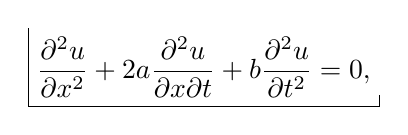
\begin{tikzpicture}
\node[inner sep=3pt] (pde) at (0,0)
  {$\displaystyle\frac{\partial^2u}{\partial x^2}
    +2a\frac{\partial^2u}{\partial x\partial t}
    +b\frac{\partial^2u}{\partial t^2}=0,$};
\draw (pde.north west) -- (pde.south west) -- (pde.south east) -- ++(0,4pt);
\end{tikzpicture}}\endgroup}
\end{GelfandAdjacentEvidence}
\begin{GelfandAdjacentEvidence}{GELFAND-P000473}{3}

\[
\begin{gathered}
0<x<\pi\\
0\leqslant t<+\infty
\end{gathered}
\]
\Unclear{GELFAND-P000473}{top-time-inequality}{Второй знак неравенства густо наведён. Условное чтение $0\leqslant t<+\infty$.}
\end{GelfandAdjacentEvidence}
\begin{GelfandAdjacentEvidence}{GELFAND-P000473}{4}

\uline{Пусть эллипт. ур-е.}
\Unclear{GELFAND-P000473}{elliptic-heading}{Первое слово читается «Пусть».}
\end{GelfandAdjacentEvidence}
\begin{GelfandAdjacentEvidence}{GELFAND-P000473}{5}


\[
\underline{a^2<b};\qquad\underline{b>0}.
\]
\[
v_k(x)=e^{\gamma kx}\sin kx,\qquad
\gamma=\frac{-a}{\sqrt{b-a^2}};\qquad k=\pm1,\ \pm2,\ \ldots .
\]
\SourceFigure{GELFAND-P000473}{gamma-bracket}{Под формулой для $\gamma$ рамочная черта с загнутыми концами.}
\end{GelfandAdjacentEvidence}
\begin{GelfandAdjacentEvidence}{GELFAND-P000473}{6}


1. Система полна, но неизв., как находить коэффициенты.
Это вопрос о нахожд. биортог. системы.
\Unclear{GELFAND-P000473}{upper-system-correction}{Окончание слова «системы» наведено. После точки отдельный зачёркнутый знак.}
\end{GelfandAdjacentEvidence}
\begin{GelfandAdjacentEvidence}{GELFAND-P000473}{7}

(нах. в терминах обр. ф-и к интегр. Кристоффеля–Шварца)

(\uline{биортог. система есть})

2. \uline{Это не базис!} (не любой вектор разлаг. в сход. ряд по этой сист.)

\sout{Даже}\quad\uline{Более того:} если есть разл. в $L^2$,
то предел — аналит. ф-я! — и вып. беск. число краев. условий (верно и обратное).
\Unclear{GELFAND-P000473}{middle-cancelled-even}{Зачёркнутое слово предположительно «Даже».}
\end{GelfandAdjacentEvidence}
\begin{GelfandAdjacentEvidence}{GELFAND-P000473}{8}


Нельзя суммировать методом Абеля 1-го порядка.

\uline{если}
\[
\sum_{\lambda_k>0}e_k e^{\lambda_k t}v_k(x)
\]
\Unclear{GELFAND-P000473}{middle-abel-coefficient}{Коэффициент густо наведён; условное чтение $e_k$.}
\end{GelfandAdjacentEvidence}
\begin{GelfandAdjacentEvidence}{GELFAND-P000473}{9}

\Incomplete{GELFAND-P000473}{middle-abel-cancelled}{Два коротких фрагмента после $v_k(x)$ густо зачёркнуты. Чтение не установлено.}
\end{GelfandAdjacentEvidence}
\begin{GelfandAdjacentEvidence}{GELFAND-P000473}{10}

им. предел при $t\to0$,
то \uwave{ф-я предельная} аналитична.
\SourceFigure{GELFAND-P000473}{limiting-function-line}{Волнистая черта проходит над «ф-я» и под «предельная».}
\end{GelfandAdjacentEvidence}
\begin{GelfandAdjacentEvidence}{GELFAND-P000473}{11}


(Дискредитация метода Фурье для эллипт. ур-я)

При нек-рых неразд. условиях можно решать.
\Unclear{GELFAND-P000473}{boundary-abbreviation}{Перед «условиях» читается сокращение «неразд.».}
\end{GelfandAdjacentEvidence}
\begin{GelfandAdjacentEvidence}{GELFAND-P000473}{12}


\Incomplete{GELFAND-P000473}{lower-cancelled-marks}{Перед «Причина» видны две зачёркнутые пометы. Чтение не установлено.}
\end{GelfandAdjacentEvidence}
\begin{GelfandAdjacentEvidence}{GELFAND-P000473}{13}

\uline{Причина плохого повед.:} резольвента $\exp$ растёт в углах
\SourceFigure{GELFAND-P000473}{resolvent-angle-diagram}{Две пересекающиеся линии, прерывистые штрихи слева, точка на пересечении, кружок и стрелка справа.\par\smallskip\centering
\begingroup\color{black}\GelfandFitDiagram{\begin{tikzpicture}[>=stealth]
\draw (-2.15,.35) -- (1.41,-.27);
\draw (-1.84,-.6) -- (1.51,.37);
\draw[densely dotted] (-2.21,-.15) -- (-.91,.02);
\fill (0,0) circle (1.3pt);
\draw (.82,.035) ellipse (.065 and .025);
\draw[->] (1.14,.025) -- (1.76,.07);
\end{tikzpicture}}\endgroup}
\end{GelfandAdjacentEvidence}
\begin{GelfandAdjacentEvidence}{GELFAND-P000473}{14}


На $[0,\pi-\varepsilon]$ переопределена.

На $[0,\pi+\varepsilon]$, $0<\varepsilon<\pi$ она остаётся полной !!! (И. Бернштейн)
\Unclear{GELFAND-P000473}{epsilon-lower-bound}{Нижняя граница густо наведена и условно набрана как ноль.}
\end{GelfandAdjacentEvidence}


На $[0,2\pi]$ возникает много ортог. ф-ий.

\uline{Задача теории целых ф-ий.}
\[
\int_0^\pi f(x)e^{\gamma kx}\sin kx\,dx=0
\quad\Longrightarrow\quad
F(\lambda)=\int_0^\pi f(x)e^{\gamma\lambda x}\sin\lambda x\,dx
\]
$F(\lambda)$ целая ф-я $\exp$ типа. Она 0 в целых точках
$F(n)=0$, $n>0$.

\uline{Надо учесть специфику.}

На $[0,\pi-\varepsilon]$ срабатывает тип и индик. диаграмма.

Единственность — ?

Неизвестно, что будет, если заменить $k$ на $\lambda_k$.


\Needspace{7\baselineskip}
\begin{GelfandAdjacentEvidence}{GELFAND-P000474}{1}
\SourcePage{GELFAND-P000474}{unlabelled}
\uuline{И. М. Гельфанд}\qquad\uuline{о раб. Арнольда.}
\SourceFigure{GELFAND-P000474}{gelfand-arnold-heading}{Имя и тема дважды подчёркнуты.}
\end{GelfandAdjacentEvidence}
\begin{GelfandAdjacentEvidence}{GELFAND-P000474}{2}

\[
(\mathbb R^n,0)\longrightarrow(\mathbb R,0)
\]
$f(x)=0$ — гиперпов.

Как ведёт себя гиперпов. в окр. $0$ — ?

$f\in C^\infty$;\quad $f(0)=0$, $df(0)=0$. (крит. точка).

(На самом деле рассм. $\mathbb C^n\longrightarrow\mathbb C$)

Эквив. гиперпов. — отлич. заменой переменных
\[
(\mathbb R^n,0)\longrightarrow(\mathbb R^n,0)\qquad
\text{(диффеом.)}.
\]

\uline{Простая гиперпов.:}\qquad\uline{\mbox{$f(x)=0$}}

если пошевелить, то будет конечное число орбит
в струях пор. $N$ (оценка числа орбит не зависит от номера $N$).

Перечисление простых орбит:
\SourceFigure{GELFAND-P000474}{simple-chain-graphs}{Слева две цепочки. В конце нижней цепочки развилка.\par\smallskip\centering
\begingroup\color{black}\GelfandFitDiagram{\begin{tikzpicture}[vertex/.style={circle,draw,inner sep=1.45pt}]
\node[vertex] (a0) at (0,0) {};
\node[vertex] (a1) at (.75,0) {};
\node[vertex] (a2) at (1.45,0) {};
\node[vertex] (a3) at (2.02,0) {};
\node[vertex] (a4) at (4.23,0) {};
\draw (a0)--(a1)--(a2)--(a3)--(2.49,0);
\node at (2.95,0) {$\cdots$};
\draw (3.66,0)--(a4);
\node[vertex] (d0) at (-.15,-.82) {};
\node[vertex] (d1) at (.62,-.82) {};
\node[vertex] (d2) at (4.15,-.82) {};
\node[vertex] (d3) at (4.54,-.55) {};
\node[vertex] (d4) at (4.54,-1.09) {};
\draw (d0)--(d1)--(1.26,-.82);
\node at (1.81,-.82) {$\cdots$};
\draw (3.44,-.82)--(d2)--(d3);
\draw (d2)--(d4);
\end{tikzpicture}}\endgroup}
\end{GelfandAdjacentEvidence}
\begin{GelfandAdjacentEvidence}{GELFAND-P000474}{3}

\SourceFigure{GELFAND-P000474}{exceptional-graphs}{Справа цепочка с нижним ответвлением у третьей вершины. Последние звенья прерывистые.\par\smallskip\centering
\begingroup\color{black}\GelfandFitDiagram{\begin{tikzpicture}[vertex/.style={circle,draw,inner sep=1.35pt}]
\node[vertex] (e0) at (0,0) {};
\node[vertex] (e1) at (.68,0) {};
\node[vertex] (e2) at (1.14,0) {};
\node[vertex] (e3) at (1.66,0) {};
\node[vertex] (e4) at (2.17,0) {};
\node[vertex] (e5) at (2.98,0) {};
\node[vertex] (e6) at (3.76,0) {};
\node[vertex] (e7) at (1.14,-.53) {};
\draw (e0)--(e1)--(e2)--(e3)--(e4);
\draw (e2)--(e7);
\draw[densely dotted] (e4)--(e5)--(e6);
\node[right] at (4.14,-.06) {$E_6,E_7$ и $E_8$};
\end{tikzpicture}}\endgroup}
\end{GelfandAdjacentEvidence}
\begin{GelfandAdjacentEvidence}{GELFAND-P000474}{4}


Далее: Большинство орбит простые (как правило, орбита-простая).
\Incomplete{GELFAND-P000474}{middle-parenthetic-cancelled}{После открывающей скобки зачёркнут короткий фрагмент. Чтение не установлено.}
\end{GelfandAdjacentEvidence}
\begin{GelfandAdjacentEvidence}{GELFAND-P000474}{5}

\uline{Непростые коразмерности 6.}

\[
x_1^{n+1}+x_2^2+\cdots\,\ast=0
\]
— соотв. 1-му типу.
\Unclear{GELFAND-P000474}{middle-simple-equation}{Первая буква в показателе $n+1$ наведена. После многоточия виден отдельный знак, похожий на звёздочку. Под формулой рамочная черта.}
\end{GelfandAdjacentEvidence}
\begin{GelfandAdjacentEvidence}{GELFAND-P000474}{6}


\uline{Версальная деформация.}
\[
\begin{gathered}
F(x,\lambda)=0,\qquad F(x,0)=f(x),\\
\lambda=(\lambda_1,\lambda_2,\ldots,\lambda_k)
\end{gathered}
\]
Всякая другая деф. эквив. деф., индуц. из этой след. образом:
\[
G(x,\mu)=F(X(x,\mu),\Psi(\mu))
\quad\text{и}\quad X(y,0)=y,\quad\Psi(0)=0
\]
\Unclear{GELFAND-P000474}{middle-induced-variables}{Первые аргументы $G$ и $X$ густо наведены и условно читаются как $x$. Справа ясно написано $X(y,0)=y$.}
\end{GelfandAdjacentEvidence}
\begin{GelfandAdjacentEvidence}{GELFAND-P000474}{7}


\uline{Правило построения верс. сем-ва:}
Берём орбиту и мн-ие, трансверс. к орбите.
\SourceFigure{GELFAND-P000474}{transverse-sketch}{Изогнутая линия и короткий поперечный отрезок с точкой пересечения.\par\smallskip\centering
\begingroup\color{black}\GelfandFitDiagram{\begin{tikzpicture}
\draw (-.81,-.58) .. controls (-.36,.06) and (.03,.33) .. (.94,.59);
\draw[line width=.95pt] (-.39,.3) .. controls (-.12,.11) and (-.03,-.03) .. (.04,-.22);
\fill (-.11,.12) circle (1.5pt);
\end{tikzpicture}}\endgroup}
\end{GelfandAdjacentEvidence}
\begin{GelfandAdjacentEvidence}{GELFAND-P000474}{8}

{\centering\rule{1.8em}{.4pt}\quad\textperiodcentered\quad\rule{2.4em}{.4pt}\par}

\[
F(x,\lambda)=f(x)+
\sum a_i\left.\frac{\partial F}{\partial\lambda_i}\right|_{\lambda_i=0}
=f(x)+\sum c_i\varphi_i(x)+O(\lambda^2).
\]
\Unclear{GELFAND-P000474}{lower-taylor-coefficient}{Множитель первого слагаемого суммы условно читается $a_i$. Под чертой подстановки написано $\lambda_i=0$.}
\end{GelfandAdjacentEvidence}
\begin{GelfandAdjacentEvidence}{GELFAND-P000474}{9}


\uuline{\mbox{$\varphi_i$} зад}\quad\uline{Инфинитезимальную версальную деформацию:}
если $\forall$ ф-я $a(x)$ предст. в виде
\Unclear{GELFAND-P000474}{lower-definition-heading}{Первый фрагмент густо наведён и дважды подчёркнут. Условное чтение $\varphi_i$ «зад».}
\end{GelfandAdjacentEvidence}
\begin{GelfandAdjacentEvidence}{GELFAND-P000474}{10}

\[
a(x)=\sum\underline{\underline{\frac{\partial f}{\partial x_i}}}\cdot h_i(x)
+\sum_{i=1}^{k}c_i\varphi_i(x)
\]
$a(x)$ задаёт инфинитезим. верс. деформ.

($\varphi_i$ порожд. лок. кольцо глад отобр.)

\Incomplete{GELFAND-P000474}{bottom-cancelled-taylor}{Перед скобками с записью о Тейлоре видна отдельная зачёркнутая запись. Чтение не установлено.}
\end{GelfandAdjacentEvidence}

(из разл. по Тейлору той ф-ии)

Важно: факторкольцо по \uline{якобиеву идеалу}
$\left(\left\{\dfrac{\partial f}{\partial x_i}\right\}\right)$.

\uline{Фактор} — конечномерное пр-во размерности $k$.

{\centering\rule{2.9em}{.4pt}\quad\textperiodcentered\quad\rule{3.4em}{.4pt}\par}


\Needspace{7\baselineskip}
\begin{GelfandAdjacentEvidence}{GELFAND-P000475}{1}
\SourcePage{GELFAND-P000475}{unlabelled}
\[
\underline{\underline{f=z_1^{k+1}+z_2^2+\cdots+z_n^2.}}
\]

Тогда
\[
\frac{\partial f}{\partial z_1}=z_1^k,\qquad
\frac{\partial f}{\partial z_2}=z_2,\ \ldots,
\]
\Unclear{GELFAND-P000475}{top-derivatives}{Справа написаны одночлены без числовых множителей.}
\end{GelfandAdjacentEvidence}
\begin{GelfandAdjacentEvidence}{GELFAND-P000475}{2}

отсюда факторкольцо — пр-во размерности $k$.

\[
\varphi_i=1,z_i,z_i^2,\ldots,z_1^{k-1}
\]
\Unclear{GELFAND-P000475}{top-phi-indices}{У первых двух степеней после $1$ видны индексы, похожие на $i$; у последней — $1$.}
\end{GelfandAdjacentEvidence}
\begin{GelfandAdjacentEvidence}{GELFAND-P000475}{3}


Верс. деформация:
\[
\underline{\lambda_0+\lambda_1z_1+\cdots+\lambda_{k-1}z_1^{k-1}
+z_1^{k+1}+z^2}
\quad\text{— \uline{верс. деформация}}
\]
\SourceFigure{GELFAND-P000475}{versal-bracket}{Под многочленом рамочная черта. Последнее слагаемое написано $z^2$.}
\end{GelfandAdjacentEvidence}
\begin{GelfandAdjacentEvidence}{GELFAND-P000475}{4}


{\centering\rule{2.8em}{.4pt}\quad\textperiodcentered\quad\rule{3.2em}{.4pt}\par}
\uline{\mbox{$F(z,\lambda)=0$}.}\qquad
Бифуркац. диаграмма — мн-во тех $\lambda$, где остаются особ. точки (в верс. деформации).

\SourceFigure{GELFAND-P000475}{theorem-star}{Слева от теоремы четыре отрезка пересекаются в одной точке.\par\smallskip\centering
\begingroup\color{black}\GelfandFitDiagram{\begin{tikzpicture}
\draw (-.72,.41)--(.64,-.58);
\draw (.05,.67)--(-.06,-.72);
\draw (-.96,-.27)--(.96,.16);
\draw (-1,-.62)--(.73,.46);
\end{tikzpicture}}\endgroup}
\end{GelfandAdjacentEvidence}
\begin{GelfandAdjacentEvidence}{GELFAND-P000475}{5}

\uuline{Теор.:} на откр.
\(\underset{\text{\scriptsize\tikz[baseline=(label.base)]\node[draw,ellipse,inner sep=1pt] (label) {бифурк. диагр.};}}{\text{мн-ве}}\)
уже будут простые особ. точки (морсовские).
\SourceFigure{GELFAND-P000475}{theorem-bifurcation-insertion}{Сокращение «бифурк. диагр.» вписано в выноску под «мн-ве».}
\end{GelfandAdjacentEvidence}
\begin{GelfandAdjacentEvidence}{GELFAND-P000475}{6}


\[
z_1^{k+1}+z_2^2=0
\qquad\Vert\qquad
\begin{gathered}
\text{бифурк. диагр. этой точки —}\\[-.2ex]
\longrightarrow\text{ Ласточкин хвост}.
\end{gathered}
\]
\[
\begin{gathered}
z_1^{k+1}+z_2^2+\lambda_{k-1}z_1^{k-1}+\cdots+\lambda_0\\
z_2^2=-p_{k+1}(z_1);\qquad z_2=\sqrt{-p_{k+1}(z_1)}.
\end{gathered}
\]
особ. точки\quad $(z_2,P'(z_1))=0$, т. е.
\[
\underline{P(z_1)=0\ \text{и}\ P'(z_1)=0}
\]
($P$ имеет кратные корни)
\SourceFigure{GELFAND-P000475}{multiple-root-bracket}{Оба равенства обведены снизу общей рамочной чертой.}
\end{GelfandAdjacentEvidence}
\begin{GelfandAdjacentEvidence}{GELFAND-P000475}{7}


Рассм. доп. к бифурк. диаграмме и его фунд. группу.
Она есть группа кос группы Коксетера.

Рассм. ур-е
\[
\underline{P(z,\lambda)=0,\quad |z|<\varepsilon}
\qquad\text{\uline{\mbox{$\lambda$} такое, что нет особенностей}}
\]
\Unclear{GELFAND-P000475}{middle-polynomial-name}{Первая буква густо наведена. Условное чтение $P$.}
\end{GelfandAdjacentEvidence}
\begin{GelfandAdjacentEvidence}{GELFAND-P000475}{8}


гомологии этого пр-ва $\ne0$ лишь в \sout{разм.}
\Incomplete{GELFAND-P000475}{lower-homology-cancelled}{После зачёркнутого «разм.» видны остатки записи. Полное чтение не установлено.}
\end{GelfandAdjacentEvidence}
\begin{GelfandAdjacentEvidence}{GELFAND-P000475}{9}

половинной разм. $n-1$.

Оно есть букет из $\mu$ сфер.
\SourceFigure{GELFAND-P000475}{sphere-bouquet}{Четыре петли с общей точкой изображают букет.\par\smallskip\centering
\begingroup\color{black}\GelfandFitDiagram{\begin{tikzpicture}
\draw (0,0) .. controls (-1.2,.83) and (-1.45,-.58) .. (0,0);
\draw (0,0) .. controls (-.37,1.37) and (.95,1.59) .. (0,0);
\draw (0,0) .. controls (1.7,1.32) and (1.7,-.86) .. (0,0);
\draw (0,0) .. controls (-.29,-1.73) and (-1.23,-1.45) .. (0,0);
\fill (0,0) circle (1.25pt);
\end{tikzpicture}}\endgroup}
\end{GelfandAdjacentEvidence}
\begin{GelfandAdjacentEvidence}{GELFAND-P000475}{10}


\Incomplete{GELFAND-P000475}{lower-left-cancelled}{Запись слева от $H^{n-1}$ густо зачёркнута. Чтение не установлено.}
\end{GelfandAdjacentEvidence}
\begin{GelfandAdjacentEvidence}{GELFAND-P000475}{11}

$H^{n-1}$ имеет образующие $e_1\ e_2\ldots\ e_\mu$.

Индекс пересеч. опред. скалярное произвед. $(e_i,e_k)$.

\[
n-1\equiv2\pmod4\qquad\Vert\qquad
\begin{gathered}
\text{отриц. опред.}\\
\text{полуопред.}\\
\text{неопред.}
\end{gathered}
\qquad\underline{e_i^2=-2}\quad\text{(всегда)}
\]
\Incomplete{GELFAND-P000475}{lower-signature-cancelled}{Между «полуопред.» и «неопред.» одна зачёркнутая строка. Чтение не установлено.}
\end{GelfandAdjacentEvidence}
\begin{GelfandAdjacentEvidence}{GELFAND-P000475}{12}


\uwave{монодромия}: предст. фунд. гр. в
\Incomplete{GELFAND-P000475}{lower-monodromy-cancelled}{После «в» зачёркнута запись; дальше многоточие. Чтение записи не установлено.}
\end{GelfandAdjacentEvidence}
\begin{GelfandAdjacentEvidence}{GELFAND-P000475}{13}

\ldots

{\centering\rule{4em}{1pt}\quad\textbullet\quad\rule{4em}{1pt}\par}

\sout{Атья}
\Unclear{GELFAND-P000475}{bottom-cancelled-name}{Зачёркнутое имя предположительно «Атья».}
\end{GelfandAdjacentEvidence}

\uline{Есть раб. Атья, Ботта,\ldots:} как избавиться от производных в выкладках Синг.?
Как, сидя в одной точке, изучить топологию мира? Нахожд. явного вида асимптотики для ур-й 2-го порядка (сообр. И. М. Гельфанда, В. И. Арнольда и др.)

(будет в следующем семестре)

А. Шнирельман о работах Маслова.


\Needspace{7\baselineskip}
\begin{GelfandAdjacentEvidence}{GELFAND-P000476}{1}
\SourcePage{GELFAND-P000476}{unlabelled}
\uuline{В. М. Бухштабер.} (продолжение).

\[
\begin{gathered}
A\overset{\text{аддит.}}{=}\Lambda[[X]],\qquad
X_n\text{ — аддит. образующие}\\
X_n\cdot X_m=C_{n+m}^n X_{n+m}
\end{gathered}
\]
\Unclear{GELFAND-P000476}{additive-equality}{Под «аддит.» две короткие параллельные черты, читается знак равенства.}
\end{GelfandAdjacentEvidence}
\begin{GelfandAdjacentEvidence}{GELFAND-P000476}{2}


\[
\begin{gathered}
\operatorname{Ext}_A^{2,*}(\Lambda,\Lambda)\\[-.4ex]
\rotatebox[origin=c]{90}{$=$}\\[-.4ex]
\operatorname{Ker}d_3^*/\operatorname{Im}d_2^*
\end{gathered}
\qquad\text{в терминах }B\text{-конструкции}
\]

$1^\circ$.
\[
d_3^*\colon\overline A^*\otimes\overline A^*
\longrightarrow\overline A^*\otimes\overline A^*\otimes\overline A^*
\]

\[
A^*=\operatorname{Hom}_{\Lambda}^{c}(\Lambda[[X]],\Lambda)
\overset{\text{адд.}}{\simeq}\Lambda[x]
\]
\Unclear{GELFAND-P000476}{top-dual-hom}{У $\operatorname{Hom}$ верхний индекс читается $c$, нижний — $\Lambda$.}
\end{GelfandAdjacentEvidence}
\begin{GelfandAdjacentEvidence}{GELFAND-P000476}{3}

\uuline{компактное} (ненулев. знач. на конечн. числе).
\SourceFigure{GELFAND-P000476}{compact-annotation}{Пояснение «компактное» написано под $\operatorname{Hom}$ и соединено с ним штрихом.}
\end{GelfandAdjacentEvidence}
\begin{GelfandAdjacentEvidence}{GELFAND-P000476}{4}


\[
\begin{gathered}
\Delta\colon A^*\longrightarrow A^*\otimes A^*\\
\Delta x_n\longrightarrow x_n\otimes1+1\otimes x_n+\sum d_{i,j}x_i\otimes x_j^*
\end{gathered}
\]
\Unclear{GELFAND-P000476}{top-delta-star}{После $x_j$ видна звёздочка. В следующей формуле для $\Delta x_n$ звёздочки нет.}
\end{GelfandAdjacentEvidence}
\begin{GelfandAdjacentEvidence}{GELFAND-P000476}{5}


\[
\begin{aligned}
(\Delta x_n,x_i\otimes x_j)&=d_{i,j}\\[-.4ex]
\qquad\rotatebox[origin=c]{90}{$=$}&\\[-.4ex]
(x_n,x_i\cdot x_j)&=(x_n,C_{i+j}^{i}x_{i+j})=C_{i+j}^{i}\delta_{n,i+j}
\end{aligned}
\]
\SourceFigure{GELFAND-P000476}{pairing-layout}{Две строки скалярного спаривания соединены вертикальным знаком равенства.}
\end{GelfandAdjacentEvidence}
\begin{GelfandAdjacentEvidence}{GELFAND-P000476}{6}


\[
\Delta x_n=x_n\otimes1+1\otimes x_n+\sum C_n^i x_i\otimes x_{n-i}
\]
И положим\quad $x_n=x^n$
\[
\begin{gathered}
\Delta x^n=(x\otimes1+1\otimes x)^n\\
d_3^*\colon \overline{\Lambda[x,y]}\longrightarrow\overline{\Lambda[x,y,z]}
\end{gathered}
\]

\[
d_3\Biggl(\underset{
  \substack{\rotatebox[origin=c]{90}{$=$}\\ \sum h_{i,j}x^iy^j}
}{h(x,y)}\Biggr)=\sum h_{ij}(\overline\Delta x^i)z^j
-\sum h_{i,j}x^i\overline\Delta y^j=
\]
\Unclear{GELFAND-P000476}{middle-differential-star}{В вычислении перед $h(x,y)$ стоит $d_3$ без звёздочки. В предыдущей строке написано $d_3^*$.}
\end{GelfandAdjacentEvidence}
\begin{GelfandAdjacentEvidence}{GELFAND-P000476}{7}


\[
\overline\Delta x^n=
\underset{\substack{
 \rotatebox[origin=c]{90}{$=$}\\
 (\Delta(x))^n\\
 \rotatebox[origin=c]{90}{$=$}\\
 (x+y)^n
}}{\Delta x^n}-x^n-y^n.
\]
\SourceFigure{GELFAND-P000476}{coproduct-identifications}{Под $\Delta x^n$ вертикальными знаками равенства соединены $(\Delta(x))^n$ и $(x+y)^n$.}
\end{GelfandAdjacentEvidence}
\begin{GelfandAdjacentEvidence}{GELFAND-P000476}{8}


\[
=h(x+y,z)-\mbox{\sout{\ensuremath{h(x,z)}}}-h(y,z)
-h(x,y+z)+h(x,y)+\mbox{\sout{\ensuremath{h(x,z)}}}.
\]
\SourceFigure{GELFAND-P000476}{cancelled-cocycle-terms}{Оба вхождения $h(x,z)$ перечёркнуты. Знаки минус и плюс перед ними видны.}
\end{GelfandAdjacentEvidence}
\begin{GelfandAdjacentEvidence}{GELFAND-P000476}{9}


\uuline{\mbox{$\operatorname{Ker}d_3^*$}:}
\[
\boxed{h(x+y,z)+h(x,y)=h(x,y+z)+h(y,z)}
\]
Эти циклы обозн. $L$.
\SourceFigure{GELFAND-P000476}{kernel-relation-box}{Равенство заключено в прямоугольную рамку.}
\end{GelfandAdjacentEvidence}
\begin{GelfandAdjacentEvidence}{GELFAND-P000476}{10}


Это и есть лазаровское соотношение.
\Unclear{GELFAND-P000476}{lazard-name}{Перед «соотношение» читается «лазаровское».}
\end{GelfandAdjacentEvidence}


\[
\underline{\operatorname{Im}d_2^*}=\Lambda\{d_2^*x^n\}
\]
\[
0\longrightarrow\operatorname{Im}d_2^*\longrightarrow L
\longrightarrow\operatorname{Ext}_A^{2,n}(\Lambda,\Lambda)\longrightarrow0
\]

\uline{Счёт группы \mbox{$\operatorname{Ext}$}.}

В ур-ии не фигурирует $\Lambda$. Поэтому дост. счит. 2 случая:

1)\quad $\Lambda$ — $Z_p$-модуль ($p$ — простое)

2)\quad $\Lambda=Q$


\Needspace{7\baselineskip}
\begin{GelfandAdjacentEvidence}{GELFAND-P000477}{1}
\SourcePage{GELFAND-P000477}{unlabelled}
остаётся\quad $X_{p^i}$

\[
\underline{A=\widehat{\prod}\otimes A_i},\qquad
A_i=Z_p[X_{p^i}]/(X_{p^i}^p)\underset{Z_p}{\otimes}\Lambda
\]
\Unclear{GELFAND-P000477}{top-tensor-product}{Над знаком произведения стоит крышка. Справа вплотную написано $\otimes$.}
\end{GelfandAdjacentEvidence}
\begin{GelfandAdjacentEvidence}{GELFAND-P000477}{2}


\[
\begin{gathered}
H^*(A_i)=\Lambda_p(u_i)\otimes Z_p[v_i],\qquad
\deg u_i=p^i,\quad\deg v_i=p^{i+1}\\
u_i\in\operatorname{Ext}^{1,p^i};\qquad
v_i\in\operatorname{Ext}^{2,p^{i+1}}
\end{gathered}
\]
\[
\operatorname{Ext}_A^{2,*}=
\left\{\underbrace{u_i u_j,\quad i<j,\quad v_k}_{\text{\uline{образующие}}}\right\}.
\]
\Unclear{GELFAND-P000477}{top-generator-inequality}{Знак между $i$ и $j$ густо наведён. Условное чтение $i<j$.}
\end{GelfandAdjacentEvidence}
\begin{GelfandAdjacentEvidence}{GELFAND-P000477}{3}


\sout{Это}\quad Но:
нужны симметрич.\quad \uline{\mbox{$h(x,y)=h(y,x)$}}
\Unclear{GELFAND-P000477}{middle-cancelled-word}{Зачёркнутое слово перед «Но» предположительно «Это».}
\end{GelfandAdjacentEvidence}
\begin{GelfandAdjacentEvidence}{GELFAND-P000477}{4}


\uuline{Бывают некоммут. одномерные группы!!}\qquad (если есть кручение)

(соотв. циклам $u_i u_j$)

\uline{Пример:}\quad $x+y+axy^p$, где $a^2=0$ \quad
над $Z_p[a]/(a^2)$.
\SourceFigure{GELFAND-P000477}{formal-group-law}{Слагаемое $axy^p$ и условие $a^2=0$ написаны в одной строке.}
\end{GelfandAdjacentEvidence}
\begin{GelfandAdjacentEvidence}{GELFAND-P000477}{5}

Это некоммут. форм. группа!!

Их столько, сколько циклов.

$v_k$ соотв. коммут. группы
\[
h(x,y)=(x+y)^{p^{k+1}}-x^{p^{k+1}}-y^{p^{k+1}}
\]
коэфф. дел. на $p$ (только)
\Unclear{GELFAND-P000477}{bottom-divisibility-word}{Слово в скобках читается «только».}
\end{GelfandAdjacentEvidence}
\begin{GelfandAdjacentEvidence}{GELFAND-P000477}{6}


\SourceFigure{GELFAND-P000477}{lazard-polynomial-bracket}{Под формулой проведена линия с загнутыми вверх концами.\par\smallskip\centering
\begingroup\color{black}\GelfandFitDiagram{\begin{tikzpicture}
\node[inner sep=3pt] (formula) at (0,0)
 {$\displaystyle L_{p^{k+1}}(x,y)=\frac{h(x,y)}{p}$};
\draw (formula.south west) ++(0,5pt) -- (formula.south west)
 -- (formula.south east) -- ++(0,5pt);
\end{tikzpicture}}\endgroup}
\end{GelfandAdjacentEvidence}
\begin{GelfandAdjacentEvidence}{GELFAND-P000477}{7}


\uline{(в \mbox{$\forall$} размерности по 1-й образующей)}

\uwave{В этом семестре конец.}
\SourceFigure{GELFAND-P000477}{semester-ending}{Последняя строка подчёркнута волнистой и прерывистой прямой чертами.}
\end{GelfandAdjacentEvidence}



\Needspace{7\baselineskip}
\begin{GelfandAdjacentEvidence}{GELFAND-P000478}{1}
\SourcePage{GELFAND-P000478}{unlabelled}
\uline{12/\mbox{$\overline{\underline{\mathrm{II}}}$}-73г.}
\qquad\uline{Сем. Гельфанда.}

\uline{План:}\quad 1. Бухштабер, Мищенко: Топология (раб. Сулливана)

\hspace*{3.5em}2. Раб. Делиня, Ленглендса

\uline{В. Бухштабер.}\qquad\uline{О 1-й раб. Сулливана.}

$M^n$ — мн-зие

Гладкость $M^n$ — это гл. мн-зие $N^n$ и гомот. эквив.
$N^n\xrightarrow{f}M^n$
\SourceFigure{GELFAND-P000478}{smoothings-diagram}{Три стрелки соединяют два гладких многообразия и общее многообразие.\par\smallskip\centering
\begingroup\color{black}\GelfandFitDiagram{\begin{tikzpicture}[>=stealth]
\node (n1) at (0,0) {$N_1^n$};
\node (n2) at (0,-1.3) {$N_2^n$};
\node (m) at (2.35,0) {$M^n$};
\draw[->] (n1) -- node[above] {$f_1$} (m);
\draw[->] (n1) -- node[left] {$g$} (n2);
\draw[->] (n2) -- node[below right] {$f_2$} (m);
\end{tikzpicture}}\endgroup}
\end{GelfandAdjacentEvidence}
\begin{GelfandAdjacentEvidence}{GELFAND-P000478}{2}

Эквивал. $\Longleftrightarrow\exists$ диффеом. $g$, такой, что этот квадрат коммутативен (гомотопически).

$S(M^n)$ — мн-во классов эквив. гладкостей.

\Incomplete{GELFAND-P000478}{top-milnor-cancelled}{Короткая запись над «Милнор» густо зачёркнута. Чтение не установлено.}
\end{GelfandAdjacentEvidence}
\begin{GelfandAdjacentEvidence}{GELFAND-P000478}{3}

\uline{Милнор:}\quad $\operatorname{Card}S'(S^7)=28$.
\Unclear{GELFAND-P000478}{milnor-cardinality}{Между первым $S$ и скобкой виден штрих. Набрано $S^{\prime}$.}
\end{GelfandAdjacentEvidence}
\begin{GelfandAdjacentEvidence}{GELFAND-P000478}{4}


Описание\quad $S(M^n)$ — ?

\uline{Сулливан} рассм. в $M^n$ фиксир. кусочно-линейную структуру.
\par\hfill ($M^n$ — полиэдр)

\uwave{и решил зд. в этой постановке:}

(вместо диффеом. — кусочно-лин.
\Incomplete{GELFAND-P000478}{middle-cancelled-homeo}{После «кусочно-лин.» видна густо зачёркнутая запись. Чтение не установлено.}
\end{GelfandAdjacentEvidence}
\begin{GelfandAdjacentEvidence}{GELFAND-P000478}{5}

гомеоморфизм)

Получ.\quad $PL(M^n)$.

Здесь всегда\quad\uuline{\mbox{$PL(S^n)=\{S^n\}$}}
— там, где решена пробл. Пуанкаре (при $n\geqslant5$).

Рассм. на $M^n$
\(\overset{\text{\scriptsize\tikz[baseline=(word.base)]\node[draw,ellipse,inner sep=1pt] (word) {Вект.};}}{\vphantom{x}}\)
расслоение $\xi$, стабильное (большой разм.).
\Incomplete{GELFAND-P000478}{middle-vector-cancelled}{Старая запись перед «расслоение» закрашена. Над ней вписано «Вект.».}
\end{GelfandAdjacentEvidence}
\begin{GelfandAdjacentEvidence}{GELFAND-P000478}{6}


\sout{несколько степен. тривиальное}
\Unclear{GELFAND-P000478}{middle-cancelled-phrase}{Под зачёркиванием условно читается «несколько степен. тривиальное».}
\end{GelfandAdjacentEvidence}
\begin{GelfandAdjacentEvidence}{GELFAND-P000478}{7}


$T_\xi$ — комплекс Тома рассл. $\xi$,
\SourceFigure{GELFAND-P000478}{thom-quotient-bracket}{Формула ограничена снизу чертой с поднятыми концами.\par\smallskip\centering
\begingroup\color{black}\GelfandFitDiagram{\begin{tikzpicture}
\node[inner sep=3pt] (quotient) at (0,0) {$\displaystyle T_\xi=\frac{D(\xi)}{S(\xi)}$};
\draw (quotient.south west) ++(0,7pt) -- (quotient.south west)
 -- (quotient.south east) -- ++(0,7pt);
\end{tikzpicture}}\endgroup}
\end{GelfandAdjacentEvidence}
\begin{GelfandAdjacentEvidence}{GELFAND-P000478}{8}

\[
\begin{gathered}
D\text{ — рассл. шаров},\\
S\text{ — рассл. сфер}.
\end{gathered}
\]

$\dim\xi=m$.
\[
\underset{\substack{\vert\\ \text{\uline{в точке.}}}}{S^m}
 \overset{i}{\subset}T_\xi
\]
\SourceFigure{GELFAND-P000478}{point-inclusion}{Пояснение «в точке» соединено штрихом с левой сферой.}
\end{GelfandAdjacentEvidence}
\begin{GelfandAdjacentEvidence}{GELFAND-P000478}{9}

\SourceFigure{GELFAND-P000478}{bundle-fibre-diagram}{В правой схеме точка отображается включением в основание.\par\smallskip\centering
\begingroup\color{black}\GelfandFitDiagram{\begin{tikzpicture}[>=stealth]
\node (r) at (0,0) {$\mathbb R^m$};
\node (xi) at (1.85,0) {$\xi$};
\node (point) at (0,-1.25) {$*$};
\node (base) at (1.85,-1.25) {$M^n$};
\draw[->] (r) -- (xi);
\draw[->] (r) -- (point);
\draw[->] (xi) -- (base);
\draw[->] ([xshift=3pt]point.east) .. controls (.67,-1.05) and (.55,-1.25) .. (.81,-1.25) -- (base);
\end{tikzpicture}}\endgroup}
\end{GelfandAdjacentEvidence}
\begin{GelfandAdjacentEvidence}{GELFAND-P000478}{10}


Рассл. $\xi$ наз. $J$-тривиальным, если $\exists$ отобр. $\varphi$; такое что

\SourceFigure{GELFAND-P000478}{lower-j-diagram}{Над первой стрелкой различимо $i$. Знак у правой сферы и большая зачёркнутая запись справа не читаются. Дуга от левой сферы к правой подписана $1$.\par\smallskip\centering
\begingroup\color{black}\GelfandFitDiagram{\begin{tikzpicture}[>=stealth]
\node (left) at (0,0) {$S^m$};
\node (thom) at (2.35,0) {$T_\xi$};
\node (right) at (4.7,0) {$S^m$};
\draw[->] (left) -- node[above] {$i$} (thom);
\draw[->] (thom) -- node[above] {$\varphi$} (right);
\draw[->] (left.south) .. controls (.3,-1.36) and (3.87,-1.22)
 .. node[below,pos=.49] {$1$} (right.south);
\end{tikzpicture}}\endgroup}
\end{GelfandAdjacentEvidence}
\begin{GelfandAdjacentEvidence}{GELFAND-P000478}{11}

(гомот.)

т. е.\quad $\deg(\varphi\cdot i)=1$
\Unclear{GELFAND-P000478}{degree-composite}{Между $\varphi$ и $i$ видна точка.}
\end{GelfandAdjacentEvidence}


(от выбора $*$ ничего не зависит, т. к. $M^n$ предполаг. связным).

$K_J(M^n)$ — группа стаб. рассл. над $M^n$, каждое из к-рых $J$-тривиально


\Needspace{7\baselineskip}
\begin{GelfandAdjacentEvidence}{GELFAND-P000479}{1}
\SourcePage{GELFAND-P000479}{unlabelled}
\uline{Теор. Атьи:} (Мат. $10\colon5$)
\SourceFigure{GELFAND-P000479}{atiyah-heading}{После имени указан краткий ссылочный номер «Мат. 10:5».}
\end{GelfandAdjacentEvidence}
\begin{GelfandAdjacentEvidence}{GELFAND-P000479}{2}


стр. отобр.
\Incomplete{GELFAND-P000479}{top-erasure}{Первая буква зачёркнутой записи похожа на $S$. Полное чтение не установлено.}
\end{GelfandAdjacentEvidence}
\begin{GelfandAdjacentEvidence}{GELFAND-P000479}{3}

\[
\underline{S(M^n)\longrightarrow K_J(M^n).}
\]

\[
N^n\longrightarrow M^n\qquad\text{\uwave{разность.}}
\]

\sout{Сулливан:}
\[
\mbox{\sout{\ensuremath{0\longrightarrow PL(M^n)\longrightarrow K_{PLJ}(M^n)}}}
\]
\sout{всегда}
\SourceFigure{GELFAND-P000479}{sullivan-crossed-sequence}{Зачёркнуты имя, последовательность и слово «всегда». Они читаются под штрихами.}
\end{GelfandAdjacentEvidence}
\begin{GelfandAdjacentEvidence}{GELFAND-P000479}{4}


и
\[
0\longrightarrow PL(M^n)\longrightarrow K_{PLJ}(M^n)
\]
\Incomplete{GELFAND-P000479}{line-erasure}{После второго $K_{PLJ}(M^n)$ зачёркнута запись, возможно $\to0$.}
\end{GelfandAdjacentEvidence}
\begin{GelfandAdjacentEvidence}{GELFAND-P000479}{5}

\[
\text{при}\quad n\not\equiv 0,2\bmod4
\]
\Unclear{GELFAND-P000479}{dimension-congruence}{В знаке сравнения три горизонтальные черты перечёркнуты одним штрихом.}
\end{GelfandAdjacentEvidence}
\begin{GelfandAdjacentEvidence}{GELFAND-P000479}{6}

\[
\begin{array}{lll}
n\equiv0\bmod4 & \text{коядро} & Z\\
n\equiv2\quad\text{—\kern.1em//\kern.1em—} & \text{—\kern.1em//\kern.1em—} & Z_2.
\end{array}
\]
\SourceFigure{GELFAND-P000479}{cokernel-ditto}{Во второй строке два знака повтора, под «mod 4» и «коядро».}
\end{GelfandAdjacentEvidence}
\begin{GelfandAdjacentEvidence}{GELFAND-P000479}{7}


Сулливан выч. гомот. групп предст. пр-ва $K_{PLJ}(M^n)$.
\Unclear{GELFAND-P000479}{group-word}{В слове «групп» наведена петля нижнего штриха. Последняя буква допускает чтение как повторное «п».}
\end{GelfandAdjacentEvidence}


Для $K_J(M^n)$ не сделано. Послед. для $S(M^n)$ тоже есть.


\Needspace{7\baselineskip}
\begin{GelfandAdjacentEvidence}{GELFAND-P000480}{1}
\SourcePage{GELFAND-P000480}{unlabelled}
\uline{19/\mbox{$\overline{\underline{\mathrm{II}}}$}-73.}
\qquad\uuline{Р. Л. Добрушин.}
\SourceFigure{GELFAND-P000480}{field-heading}{Месяц набран римской цифрой. Под именем две линии с поперечными штрихами.}
\end{GelfandAdjacentEvidence}
\begin{GelfandAdjacentEvidence}{GELFAND-P000480}{2}


\uline{О теории поля.}

\uline{Гельфанд:}\quad 2 задачи:
{\centering\rule{1.1em}{.4pt}\quad\textperiodcentered\quad\rule{1.1em}{.4pt}\par}
1) проквантовать существующ. ур-я
\Unclear{GELFAND-P000480}{tasks-existing}{Конец сокращения условно читается «существующ.».}
\end{GelfandAdjacentEvidence}
\begin{GelfandAdjacentEvidence}{GELFAND-P000480}{3}


2) напис. ур-я, реально ответ. (физ.)
\Unclear{GELFAND-P000480}{tasks-answering}{После «реально» написано сокращение «ответ.».}
\end{GelfandAdjacentEvidence}
\begin{GelfandAdjacentEvidence}{GELFAND-P000480}{4}

{\centering\rule{1.8em}{.4pt}\quad\textperiodcentered\quad\rule{1.8em}{.4pt}\par}

\uline{Способ констр. объектов, удовл. аксиомам Уайтмана} (\uline{вероятн. объекты}).

Осн. автор — \uuline{Nelson}.

Можно (почти) получ. рез. Глимма и Джеаффе.
\Unclear{GELFAND-P000480}{jaffe-name}{В рукописи между «ж» и «а» видна буква «е», чтение «Джеаффе».}
\end{GelfandAdjacentEvidence}
\begin{GelfandAdjacentEvidence}{GELFAND-P000480}{5}


Случ. величина:\quad $\xi_t$,\quad $t\in\mathbb R^{\nu+1}$
\Unclear{GELFAND-P000480}{field-index}{Первый знак показателя похож на латинское $v$ или греческое $\nu$. Условно набрано $\nu$.}
\end{GelfandAdjacentEvidence}


1) она евкл. инвар.

2) Марк. св-во


\Needspace{7\baselineskip}
\begin{GelfandAdjacentEvidence}{GELFAND-P000481}{1}
\SourcePage{GELFAND-P000481}{unlabelled}
\uline{26/\mbox{$\overline{\underline{\mathrm{II}}}$}-73}
\qquad\uline{В. М. Бухштабер}.\qquad
$hs(M^n)$ — $\overset{\text{\scriptsize (гомотопич.)}}{\text{гладкости}}$.
\SourceFigure{GELFAND-P000481}{homotopy-smoothing-insert}{«(гомотопич.)» вписано над «гладкости», с выноской к слову.}
\end{GelfandAdjacentEvidence}
\begin{GelfandAdjacentEvidence}{GELFAND-P000481}{2}


\begingroup\color{black}\GelfandFitDiagram{\begin{tikzpicture}[baseline=(notation.base)]
\node[inner sep=2pt] (notation) at (0,0) {$ht(M^n)$};
\draw ([yshift=2pt]notation.south west) -- (notation.south west) --
  (notation.south east) -- ([yshift=2pt]notation.south east);
\node[below=5pt,inner sep=0pt] (descr) at (notation.south) {\uline{описывается.}};
\draw ([yshift=-1pt]notation.south) -- ([yshift=1pt]descr.north);
\end{tikzpicture}}\endgroup
— гомот. триангуляции.
\SourceFigure{GELFAND-P000481}{triangulation-bracket}{Надпись «описывается.» соединена чертой со скобкой под $ht(M^n)$.}
\end{GelfandAdjacentEvidence}
\begin{GelfandAdjacentEvidence}{GELFAND-P000481}{3}


\uline{Hauptvermutung} —
$\overset{\text{\scriptsize (мн-зий)}}{\text{гомеоморфизм}}$
можно заменить кусочно-лин. гомеом. (если $M$ односв. и не имеет в $H^3$ 2-кручения)
\SourceFigure{GELFAND-P000481}{hauptvermutung-insert}{«мн-зий» вписано в выноску после «гомеоморфизм».}
\end{GelfandAdjacentEvidence}
\begin{GelfandAdjacentEvidence}{GELFAND-P000481}{4}


Пусть $\alpha\in hs(M^n)$ (гом. гладкость).
\[
\alpha\underset{\text{\scriptsize сопст.}}{\mapsto}
\underbrace{\xi\longrightarrow M^n}_{\text{расслоение (вект.)}}
\qquad\text{\uline{гладкое}.}
\]
\Unclear{GELFAND-P000481}{assigned}{Под первой стрелкой условно прочитано «сопст.». Возможное чтение «сопост.».}
\end{GelfandAdjacentEvidence}
\begin{GelfandAdjacentEvidence}{GELFAND-P000481}{5}


\[
\begin{gathered}
f\colon N^n\longrightarrow M^n;\\
\exists\ g\colon M^n\longrightarrow N^n;\qquad f\circ g\sim1,\quad g\circ f\sim1.
\end{gathered}
\]
\[
\tau_{M^n}+g^*\nu_{N^n}
\qquad(\nu_{N^n}=-\tau_{N^n}\bmod\text{трив.})
\]
\Unclear{GELFAND-P000481}{normal-bundle-symbol}{Знак нормального расслоения похож на $v$. Условно набрано $\nu$.}
\end{GelfandAdjacentEvidence}
\begin{GelfandAdjacentEvidence}{GELFAND-P000481}{6}


\uline{Упр.} Док., что 2 экв. гладкости индуц. изом. расслоения $\xi$.

Получ. гладкое рассл. $\xi$ явл. $J$-тривиальным,
т. е.
\SourceFigure{GELFAND-P000481}{bundle-triviality-diagram}{Квадрат со стрелкой $\gamma$, обозначенной густо наведённым знаком.\par\smallskip
{\centering
\begingroup\color{black}\GelfandFitDiagram{\begin{tikzpicture}
\node (xi) at (0,1.25) {$\xi$};
\node (product) at (2.4,1.25) {$M^n\times R^N$};
\node (leftbase) at (0,0) {$M$};
\node (rightbase) at (2.4,0) {$M$};
\draw[->] (xi) -- node[above] {$\gamma$} (product);
\draw[->] (xi) -- (leftbase);
\draw[->] (product) -- (rightbase);
\draw[->] (leftbase) -- node[above] {$\mathrm{id}$} (rightbase);
\end{tikzpicture}}\endgroup\par}}
\end{GelfandAdjacentEvidence}
\begin{GelfandAdjacentEvidence}{GELFAND-P000481}{7}


и $\gamma$ есть собственное отобр. и гомот. эквивал.
\Unclear{GELFAND-P000481}{gamma-retracing}{Знак перед «есть» густо наведён. Условно набрано $\gamma$.}
\end{GelfandAdjacentEvidence}
\begin{GelfandAdjacentEvidence}{GELFAND-P000481}{8}


\sout{\mbox{$T(\xi)$} эквив.,}
\Unclear{GELFAND-P000481}{cancelled-word}{После зачёркнутого $T(\xi)$ условно прочитано «эквив.». Чтение «трив.» остаётся возможным.}
\end{GelfandAdjacentEvidence}
\begin{GelfandAdjacentEvidence}{GELFAND-P000481}{9}


\uuline{2-е опр.} — $\exists$ отобр.
\begingroup\color{black}\GelfandFitDiagram{\begin{tikzpicture}[baseline=(thom.base)]
\node[inner sep=1pt] (thom) {$T(\xi)$};
\node[anchor=west,inner sep=1pt] at (thom.east) {$\longrightarrow S^N$};
\node[anchor=south west,inner sep=1pt] (label) at ([xshift=1em,yshift=4pt]thom.north) {\scriptsize\uline{комп. Тома}};
\draw[->] (label.south west) -- ([yshift=1pt]thom.north);
\end{tikzpicture}}\endgroup,
такое что
\SourceFigure{GELFAND-P000481}{thom-label}{Подчёркнутая надпись «комп. Тома» со стрелкой к $T(\xi)$.}
\end{GelfandAdjacentEvidence}
\begin{GelfandAdjacentEvidence}{GELFAND-P000481}{10}


композиция
\SourceFigure{GELFAND-P000481}{thom-composite-diagram}{Нижняя стрелка обозначает композицию.\par\smallskip
{\centering
\begingroup\color{black}\GelfandFitDiagram{\begin{tikzpicture}
\node (fibre) at (0,0) {$S^N$};
\node at (0.65,0) {$\subset$};
\node (space) at (1.38,0) {$T(\xi)$};
\node (sphere) at (3.08,0) {$S^N$};
\draw[->] (space) -- (sphere);
\draw[->] (fibre.south) to[out=-30,in=-160] (sphere.south);
\end{tikzpicture}}\endgroup\par}}
\end{GelfandAdjacentEvidence}
\begin{GelfandAdjacentEvidence}{GELFAND-P000481}{11}

есть гомотопич. эквив.

Эквивалентность — теор. \uline{Дольда} (технич., идейно трив.)
\SourceFigure{GELFAND-P000481}{dold-name}{Подчёркнутое имя «Дольда».}
\end{GelfandAdjacentEvidence}



\Needspace{7\baselineskip}
\begin{GelfandAdjacentEvidence}{GELFAND-P000482}{1}
\SourcePage{GELFAND-P000482}{unlabelled}
\uuline{5/\mbox{$\overline{\underline{\mathrm{III}}}$}-73 г.}
\qquad\uline{Сем. Гельфанда}.

\uline{Теорема.}\enspace\sout{Ф. А. Березин}\qquad\uline{Ломоносов}
\Unclear{GELFAND-P000482}{cancelled-name}{Густо зачёркнутое имя условно прочитано «Ф. А. Березин».}
\end{GelfandAdjacentEvidence}
\begin{GelfandAdjacentEvidence}{GELFAND-P000482}{2}


$R$ — сем-во попарно комм.
$\overset{\text{\scriptsize (в бан. пр-ве $B$)}}{\text{опер.}}$,
содержащее вп. непр. опер. $A\ne0$.
\SourceFigure{GELFAND-P000482}{banach-space-insert}{После «опер.» в выноске вписано «в бан. пр-ве $B$».}
\end{GelfandAdjacentEvidence}
\begin{GelfandAdjacentEvidence}{GELFAND-P000482}{3}

\Unclear{GELFAND-P000482}{operator-condition}{Последний знак разомкнут справа и похож на $C$. Условно набрано $0$.}
\end{GelfandAdjacentEvidence}
\begin{GelfandAdjacentEvidence}{GELFAND-P000482}{4}


Тогда $R$ имеет общее
$\overset{\text{\scriptsize (нетрив.)}}{\text{инвариантное подпр-во}}$.
\SourceFigure{GELFAND-P000482}{nontrivial-insert}{«нетрив.» вписано между «общее» и «инвариантное».}
\end{GelfandAdjacentEvidence}
\begin{GelfandAdjacentEvidence}{GELFAND-P000482}{5}


(обобщение теоремы Ароншайна — Смита)
\SourceFigure{GELFAND-P000482}{theorem-name}{В имени читается «Ароншайна».}
\end{GelfandAdjacentEvidence}
\begin{GelfandAdjacentEvidence}{GELFAND-P000482}{6}


Док-во проходит в случае ЛВП, короткое и простое.
\Unclear{GELFAND-P000482}{proof-word-erasure}{Перед «короткое» густо зачёркнут короткий знак. Чтение не установлено.}
\end{GelfandAdjacentEvidence}
\begin{GelfandAdjacentEvidence}{GELFAND-P000482}{7}


\uline{Док-во.}\quad $S'$ —
$\underset{\text{\scriptsize (в $B$)}}{\text{замкн. шар}}$,
$r=1$ с центром в $x_0$, такой, что
\SourceFigure{GELFAND-P000482}{ball-space-insert}{Под «шар» вписано «в $B$» с выноской.}
\end{GelfandAdjacentEvidence}
\begin{GelfandAdjacentEvidence}{GELFAND-P000482}{8}

\SourceFigure{GELFAND-P000482}{ball-prime}{У первого обозначения шара $S'$ имеется штрих. Далее в рукописи стоит $S$.}
\end{GelfandAdjacentEvidence}
\begin{GelfandAdjacentEvidence}{GELFAND-P000482}{9}

\[
\inf_{x\in S}\lVert Ax\rVert>1/2
\]
\[
\begin{gathered}
Ax_0'\ne0\\
\lVert x_0'\rVert=1
\end{gathered}
\qquad\text{и берём}\qquad
\lVert A\rVert\cdot x_0'=x_0.
\]
\Unclear{GELFAND-P000482}{scaling}{Внутри двойных черт буква густо наведена. Условное чтение $\lVert A\rVert$.}
\end{GelfandAdjacentEvidence}
\begin{GelfandAdjacentEvidence}{GELFAND-P000482}{10}


$\overline{AS}$ — компакт, не содержащий нуля.

Рассм. $\overset{\mathcal R}{\text{алгебру}}$ с $1$,
порождённую сем-вом $R$ (без замыкания).
\SourceFigure{GELFAND-P000482}{algebra-insert}{Над «алгебру» вписано обозначение, условно набранное $\mathcal R$.}
\end{GelfandAdjacentEvidence}
\begin{GelfandAdjacentEvidence}{GELFAND-P000482}{11}

\[
\forall y\in B,\qquad \mathcal R y\quad\text{— лин. мн-зие}.
\]
Легко видеть, что $\mathcal R y$ инвар. отн. $\mathcal R$.

$\overline{\mathcal R y}$ — инв. подпр-во.

Надо док., что оно может быть нетрив..

Пусть $y\in\overline{AS}$. Надо пров., что $\exists y$;
$\mathcal R y$ не плотно.

Пусть не так, тогда
\Unclear{GELFAND-P000482}{then-erasure}{Зачёркнутое слово после «тогда» не разобрано. Возможное чтение «оно».}
\end{GelfandAdjacentEvidence}
\begin{GelfandAdjacentEvidence}{GELFAND-P000482}{12}

\[
\forall y\in\overline{AS}\quad\exists T\in\mathcal R,\qquad
\lVert Ty-x_0\rVert<1.
\]
Из комп. $\overline{AS}$ след. $\exists T_1,\ldots,T_n$
\[
\forall y\ \exists i\qquad\lVert T_i y-x_0\rVert<1,
\]
\[
\forall y\in AS\quad\{T_1y,\ldots,T_ny\}\cap S\ne\varnothing.
\]

Пусть $f(t)\in C(0,+\infty)$
\SourceFigure{GELFAND-P000482}{cutoff-graph}{График $f(t)$, отметки $1$ на обеих осях и точка на оси $t$.\par\smallskip
{\centering
\begingroup\color{black}\GelfandFitDiagram{\begin{tikzpicture}[x=1.1cm,y=1.1cm]
\draw[->] (-0.2,0) -- (3.35,0) node[right] {$t$};
\draw (0,0) -- (0,1.22);
\draw[thick] (0,1) -- (1,0);
\fill (1,0) circle (1.1pt);
\node[left] at (0,1) {$1$};
\node[below] at (1,0) {$1$};
\node[right] at (0.4,0.98) {$f(t)$};
\end{tikzpicture}}\endgroup\par}}
\end{GelfandAdjacentEvidence}



\Needspace{7\baselineskip}
\begin{GelfandAdjacentEvidence}{GELFAND-P000483}{1}
\SourcePage{GELFAND-P000483}{unlabelled}
Рассм.
\[
\Phi y\overset{\#}{=}
\frac{\displaystyle\sum_1^n f(\lVert T_i y-x_0\rVert)T_i y}
{\displaystyle\sum_j f(\lVert T_j y-x_0\rVert)}
\qquad(\text{вып. комб.})
\]
\Unclear{GELFAND-P000483}{definition-mark}{Перед верхней чертой равенства вписан знак, похожий на $\#$.}
\end{GelfandAdjacentEvidence}
\begin{GelfandAdjacentEvidence}{GELFAND-P000483}{2}

\[
\Phi\colon\overline{AS}\longrightarrow S
\]
Это непр. ф-я на $\overline{AS}$.

Рассм. $\Phi A\colon S\longrightarrow S$,
\Unclear{GELFAND-P000483}{after-phi-a}{После $\Phi A$ затёрт знак. Возможно, $x$.}
\end{GelfandAdjacentEvidence}
\begin{GelfandAdjacentEvidence}{GELFAND-P000483}{3}

причём образ $\Phi A$ компактен и оно непр..

По теор. Шаудера $\exists$ неподв. точка, т. е.,
\[
\sum_1^n\alpha_i T_i Ax=x,\qquad
\alpha_j=\frac{f(\lVert T_jy-x_0\rVert}
{\displaystyle\sum_i f(\lVert T_i y-x_0\rVert)}
\]
\SourceFigure{GELFAND-P000483}{weights}{В обоих аргументах видно $x_0$. В числителе после знака нормы закрывающая скобка не видна.}
\end{GelfandAdjacentEvidence}
\begin{GelfandAdjacentEvidence}{GELFAND-P000483}{4}


\uline{\mbox{$T=\sum\alpha_i T_i A$} вп. непрерывен.}

$\exists x\colon Tx=x$. Отсюда соб. вект. с соб. знач. $1$ —
нетрив. инвар. подпр-во (даже конечномерное).
Отсюда $\mathcal R$ имеет инвар. подпр-во.
\SourceFigure{GELFAND-P000483}{proof-end-mark}{В росчерке после доказательства овал над двумя перекрещенными штрихами и точка справа.\par\smallskip
{\centering
\begingroup\color{black}\GelfandFitDiagram{\begin{tikzpicture}
\draw (0,.26) ellipse (.13 and .08);
\draw (-.26,.04) -- (.28,-.27) (-.22,-.27) -- (.30,.04);
\fill (.49,-.23) circle (.45pt);
\end{tikzpicture}}\endgroup\par}}
\end{GelfandAdjacentEvidence}
\begin{GelfandAdjacentEvidence}{GELFAND-P000483}{5}


(Это не значит, что вообще есть конечномерное).

\uuline{Следствие.}
Если комм. $\overset{\text{\scriptsize (бан.)}}{\text{алгебра}}$ имеет элем.,
\SourceFigure{GELFAND-P000483}{banach-insert}{«бан.» вставлено после «комм.».}
\end{GelfandAdjacentEvidence}
\begin{GelfandAdjacentEvidence}{GELFAND-P000483}{6}

\Unclear{GELFAND-P000483}{corollary-cancel}{После «элем.» зачёркнуты знак, похожий на «и», и неразобранное слово.}
\end{GelfandAdjacentEvidence}
\begin{GelfandAdjacentEvidence}{GELFAND-P000483}{7}

$\overset{\text{\scriptsize (на к-рый)}}{\text{умн.}}$
вп. непр., то $\exists$ нетрив. идеал.
\SourceFigure{GELFAND-P000483}{multiplication-insert}{«на к-рый» вписано после «умн.».}
\end{GelfandAdjacentEvidence}
\begin{GelfandAdjacentEvidence}{GELFAND-P000483}{8}


{\centering\rule{2.1em}{.4pt}\quad\textperiodcentered\quad\rule{2.5em}{.4pt}\par}

\uuline{Хенкин.}\enspace(\uline{анонс})

Пусть в $C^n$ есть вып. обл. $D\subset C^n$, зад. ур-ем $\rho(z)<0$.
\Unclear{GELFAND-P000483}{domain-letter}{Буква $D$ перед знаком включения густо наведена.}
\end{GelfandAdjacentEvidence}
\begin{GelfandAdjacentEvidence}{GELFAND-P000483}{9}


Интегр. ф-ла Лерэ для голом. огран. ф-й:
\[
f(z)=\frac{(n-1)!}{(2\pi i)^n}
\int_{\zeta\in\partial D}
\frac{f(\zeta)\,\omega'\bigl(\frac{\partial\rho}{\partial z}(\zeta)\bigr)
\wedge\omega(\zeta)}
{\bigl(\displaystyle\sum_{k=1}^n
\frac{\partial\rho}{\partial\zeta_k}(\zeta)(\zeta_k-z_k)\bigr)^n}
\]
\Unclear{GELFAND-P000483}{leray-kernel}{Знак $\rho$ в числителе производной при $\omega'$ густо наведён.}
\end{GelfandAdjacentEvidence}
\begin{GelfandAdjacentEvidence}{GELFAND-P000483}{10}


1) Инт. типа Лерэ:
\[
f_g(z)=\cdot\ \cdot\ \int
\begin{matrix}g(\zeta)\cdots\\ \cdots\end{matrix}
\qquad g(\zeta)\ \text{— ф-я на границе.}
\]
\[
f\longrightarrow[f(\zeta)g(\zeta)-f_g(\zeta)]
\quad\text{— вп. непр. оператор}
\]
и усл. Гёльдера с показ. $1/2$

2) $\rho(z)$ — строго плюрисубгарм..
\SourceFigure{GELFAND-P000483}{domain-left}{Контур слева от «Тогда».\par\smallskip
{\centering
\begingroup\color{black}\GelfandFitDiagram{\begin{tikzpicture}[x=.85cm,y=.85cm]
\draw (0.18,1.2)
.. controls (0.02,1.38) and (-0.12,1.21) .. (-0.23,1.18)
.. controls (-0.42,1.37) and (-0.66,0.98) .. (-0.64,0.87)
.. controls (-0.53,0.72) and (-0.16,0.65) .. (-0.27,0.29)
.. controls (-0.36,0.06) and (-0.69,-0.29) .. (-0.46,-0.45)
.. controls (0.02,-0.66) and (0.61,-0.38) .. (0.72,0.19)
.. controls (0.83,0.88) and (0.48,0.58) .. (0.34,0.68)
.. controls (0.14,0.75) and (0.28,1.08) .. (0.22,1.17);
\end{tikzpicture}}\endgroup\par}}
\end{GelfandAdjacentEvidence}
\begin{GelfandAdjacentEvidence}{GELFAND-P000483}{11}


Тогда $D$ — \sout{обл.} есть замкн. подмн-зие в строго вып. обл.,
трансверс. подх. к границе.
\Unclear{GELFAND-P000483}{domain-cancel}{Условное чтение зачёркнутого слова «обл.». Возможно «область».}
\end{GelfandAdjacentEvidence}
\begin{GelfandAdjacentEvidence}{GELFAND-P000483}{12}


(следует из теор. Ока)
\SourceFigure{GELFAND-P000483}{domain-right}{Наклонный овал с внутренней дугой. Дуга подходит к верхнему краю и оканчивается вблизи нижнего.\par\smallskip
{\centering
\begingroup\color{black}\GelfandFitDiagram{\begin{tikzpicture}
\draw[rotate=32] (0,0) ellipse (.85 and .53);
\draw[line width=.75pt] (.13,.61) .. controls (.27,.40) and (.26,-.11) .. (-.05,-.50);
\end{tikzpicture}}\endgroup\par}}
\end{GelfandAdjacentEvidence}
\begin{GelfandAdjacentEvidence}{GELFAND-P000483}{13}


3) в п. 2) \uline{выпис. продолж. с подмн-зия с оценками!} (в классе огр. ф-й)

Обратное тоже верно: такое подмн-зие есть \sout{область} огр. область голоморфности.
\Unclear{GELFAND-P000483}{converse-cancel}{Условное чтение зачёркнутого слова «область». Возможно «обл.».}
\end{GelfandAdjacentEvidence}


4) \uline{Следствие:} для ф-й, ан. внутри и непр. в замыкании,
пр-во макс. идеалов $=$ замыканию области.


\Needspace{7\baselineskip}
\begin{GelfandAdjacentEvidence}{GELFAND-P000484}{1}
\SourcePage{GELFAND-P000484}{unlabelled}
\uuline{Ф. А. Березин.}

\uline{Зад. квантования.}

$M$ — симпл. мн-зие
($\omega$ — форма [нрзб.] с матр. $\omega_{ik}$;
$\omega^{ik}$ — обр. матр.)
\Unclear{GELFAND-P000484}{form-mark}{После «форма» густо наведён знак. Возможные чтения $2$ или $\xi$.}
\end{GelfandAdjacentEvidence}
\begin{GelfandAdjacentEvidence}{GELFAND-P000484}{2}

\[
[f,g]=\sum\omega^{ik}\frac{\partial f}{\partial x^i}
\frac{\partial g}{\partial x^k}
\]
Квантование: сем-во ассоц. колец $A_h$ с элементами $f(x)$ (ф-и на $M$)
\[
f_1\ast f_2=g(x\mid h)
\]
\[
\left.
\begin{aligned}
1)\quad &g(x\mid0)=f_1(x)\cdot f_2(x)\\
2)\quad &\left.\frac{\partial}{\partial h}
(f_1\ast f_2-f_2\ast f_1)\right|_{h=0}=[f_1,f_2]
\end{aligned}
\right\}\quad(\text{принцип соответствия}).
\]
Ещё ряд треб. (не столь обяз.)

3) все $A_h$ — алгебры с $1$, соотв. $f_0\equiv1$.

4) $A_h$ — алгебра со следом (опр. на выд. мн-ве элементов в $A_h$).
\Unclear{GELFAND-P000484}{trace-domain}{Окончание слова «элементов» переписано. Предыдущее чтение не установлено.}
\end{GelfandAdjacentEvidence}
\begin{GelfandAdjacentEvidence}{GELFAND-P000484}{3}

\[
\mathrm{Sp}(f_1\ast f_2)=\mathrm{Sp}(f_2\ast f_1)
\]
и
\[
\mathrm{Sp}\, f=c\int f\,d\mu,
\]
где $d\mu$ — ест. мера на мн-зии (степень $\omega$).
\SourceFigure{GELFAND-P000484}{measure-word}{В скобках читается «степень $\omega$».}
\end{GelfandAdjacentEvidence}
\begin{GelfandAdjacentEvidence}{GELFAND-P000484}{4}


Треб. мат. естеств. — \uuline{функториальность} по отн. к каноническим
Диффеоморфизмам (отн. нек-рого сем-ва отобр. — нек-рой фикс. категории).

{\centering\rule{1.9em}{.4pt}\quad\textperiodcentered\quad\rule{1.9em}{.4pt}\par}

Решение изв., когда $M\in$ опр. классу
(2 класса кэлеровых мн-зий).

\begingroup\color{black}\GelfandFitDiagram{\begin{tikzpicture}
\node[align=left,anchor=west,inner sep=4pt] (classlist) at (0,0)
  {1) обл. в $C^n$\\[2pt]2) компактные симм. мн-зия,};
\draw (classlist.north west) -- (classlist.south west) -- (classlist.south east);
\end{tikzpicture}}\endgroup
\SourceFigure{GELFAND-P000484}{class-bracket}{Оба пункта обведены общей чертой слева и снизу.}
\end{GelfandAdjacentEvidence}
\begin{GelfandAdjacentEvidence}{GELFAND-P000484}{5}


{\centering\rule{1.9em}{.7pt}\quad\textbullet\quad\rule{1.9em}{.7pt}\par}

\uline{Фоковское пр-во.}
\Unclear{GELFAND-P000484}{fock-mark}{Над началом заголовка густо закрашен знак. Чтение не установлено.}
\end{GelfandAdjacentEvidence}
\begin{GelfandAdjacentEvidence}{GELFAND-P000484}{6}

\[
M=C^n\qquad\omega=\sum dz_i\wedge d\bar z_i.
\]
Ф-и — целые ф-и $f(z,\bar z)$ (разл. по $x,y$ в ряд, всюду сход.)
\[
(f_1\ast f_2)(z,\bar z)=\frac1{h^n}
\int f_1(z,\bar v)f_2(v,\bar z)
 e^{-\frac1h(z-v)(\bar z-\bar v)}\,dv\,d\bar v
\]
Важно: строение лин. предст. этого кольца.

Пусть $\varphi(z)$ — обычные целые ф-и с усл.
\[
(\varphi,\varphi)=\frac1{h^n}
\int|\varphi(z)|^2e^{-\frac{z\bar z}{h}}\,dz\,d\bar z
<+\infty\qquad(\text{пр-во }F_2)
\]
Там действует лин. предст. кольца $A_h$:
\[
(\hat f\varphi)(z)=\frac1{h^n}\int
 f(z,v)\overline{\varphi(v)}\,
 e^{-\frac1h(v-z)\bar v}\,dv\,d\bar v,
\]
$f$ — виковский символ.
\SourceFigure{GELFAND-P000484}{wick-conjugation}{Черта стоит над $\varphi(v)$. В предшествующем множителе $f(z,v)$ черты над $v$ нет.}
\end{GelfandAdjacentEvidence}
\begin{GelfandAdjacentEvidence}{GELFAND-P000484}{7}


Ещё одно кольцо операторов:
\[
(\hat f\varphi)(z)=\frac1{h^n}\int
 \mathring{f}(v,\bar v)\varphi(v)
 e^{-\frac1h(v-z)\bar v}\,dv\,d\bar v,
\]
$\mathring{f}$ — антивиковский символ.
\[
(\hat a_k\varphi)(z)=\frac{\partial\varphi}{\partial z_k},
\qquad(\hat a_k^*\varphi)(z)=z_k\varphi.
\]
\[
\begin{aligned}
\hat f&=\sum f_{mn}\hat a^{*m}\hat a^n
&\longleftrightarrow\quad
f(z,\bar z)&=\sum f_{mn}\bar z^m z^n\\
\hat f&=\sum\mathring{f}_{mn}\hat a^n\hat a^{*m}
&\longleftrightarrow\quad
\mathring{f}(z,\bar z)&=\sum\mathring{f}_{mn}z^n\bar z^m.
\end{aligned}
\]
\Unclear{GELFAND-P000484}{ordered-erasure}{У первого $\hat f$ справа вверху затёрт знак. Возможное чтение $*$.}
\end{GelfandAdjacentEvidence}
\begin{GelfandAdjacentEvidence}{GELFAND-P000484}{8}

\Unclear{GELFAND-P000484}{ordering-bars}{Нижние показатели при первом $\hat a$ и первом $z$ густо наведены. Условное чтение $n$ в обоих местах.}
\end{GelfandAdjacentEvidence}



\Needspace{7\baselineskip}
\begin{GelfandAdjacentEvidence}{GELFAND-P000485}{1}
\SourcePage{GELFAND-P000485}{unlabelled}
Рассм. $e_{\bar v}(z)=e^{\frac1h\bar v z}$ (когерентные сост. или пуасс. векторы).

\sout{\mbox{$f\ldots$}}
\Unclear{GELFAND-P000485}{upper-erasure}{В зачёркнутой записи видна буква $f$. Остальное не разобрано.}
\end{GelfandAdjacentEvidence}
\begin{GelfandAdjacentEvidence}{GELFAND-P000485}{2}


Рассм. теперь
\[
\begin{aligned}
\hat f\longleftrightarrow f(v,\bar v)
&=\frac{(\hat f e_{\bar v},e_v)}{(e_{\bar v},e_v)}
\quad\text{(распространение)}={}\\
&=\operatorname{Sp}(\hat fP_v).
\end{aligned}
\]
\SourceFigure{GELFAND-P000485}{coherent-subscripts}{В обеих строках дроби у первого $e$ индекс $\bar v$, у второго $e$ индекс $v$.}
\end{GelfandAdjacentEvidence}
\begin{GelfandAdjacentEvidence}{GELFAND-P000485}{3}


($P_v$ — ортог. проект. на $e_v$)
\[
\hat f=\int\mathring f(v,\bar v)P_v\,dv\,d\bar v
\qquad\text{(распр. антивик. символов).}
\]

\uwave{Двойственность:}

1.
\[
\begin{array}{llll}
\text{вик.} & \uparrow & \text{оп.}\longrightarrow\text{символ}\\
\text{антивик.} && \text{симв.}\longrightarrow\text{оператор}
\end{array}
\]
\SourceFigure{GELFAND-P000485}{duality-vertical-mark}{Перед «оп.» густо наведена стрелка вверх к волнистому подчёркиванию. Её связь с двумя строками не установлена.}
\end{GelfandAdjacentEvidence}
\begin{GelfandAdjacentEvidence}{GELFAND-P000485}{4}


2.
\[
\begin{aligned}
\hat f\text{ — огр.}&\Longrightarrow f\text{ огр.}\\
\mathring f\text{ — огр.}&\Longrightarrow\hat f\text{ огр.}
\end{aligned}
\]

3.
\[
\begin{aligned}
\hat f\text{ комп.}&\Longrightarrow f\to0\\
\mathring f\to0&\Longrightarrow\hat f\text{ комп.}
\end{aligned}
\]
\Unclear{GELFAND-P000485}{decay-arrow}{Стрелка к $0$ во второй строке густо наведена. Условно набрана $\to$.}
\end{GelfandAdjacentEvidence}
\begin{GelfandAdjacentEvidence}{GELFAND-P000485}{5}


4. Ядерность (анал.)
\[
\operatorname{Sp}\hat f
 =\frac1{h^n}\int f(z,\bar z)\,dz\,d\bar z
 =\frac1{h^n}\int\mathring f(z,\bar z)\,dz\,d\bar z.
\]

\uline{Ф-ла перехода:}
\[
f(z,\bar z)=\frac1{h^n}\int\mathring f(v,\bar v)
 e^{-\frac1h(z-v)(\bar z-\bar v)}\,dv\,d\bar v.
\]
При $h/2$ получается символ Вейля.
(Замеч. Гельфанда:
$\overset{\text{\scriptsize (это символы)}}{\text{Пуанкаре}}$.)
\SourceFigure{GELFAND-P000485}{poincare-insert}{«это символы» вписано сверху перед «Пуанкаре».}
\end{GelfandAdjacentEvidence}
\begin{GelfandAdjacentEvidence}{GELFAND-P000485}{6}


\uuline{Общая конструкция.}

$H$ — гильб. пр-во, $M$ — мн-во с мерой, $\alpha\in M$, мера $d\alpha$.

$e_\alpha$ — переполн. сист., если
\[
(f,f)=\int |(f,e_\alpha)|^2\,d\alpha.
\]
Рассм. тогда соответствие:
\[
\hat A\longrightarrow\frac{(\hat A e_\alpha,e_\alpha)}{(e_\alpha,e_\alpha)}
 =\underset{\substack{\vert\!\vert\\\operatorname{Sp}(\hat A\hat P_\alpha)}}{A(\alpha)}
 \qquad\text{(ковар. символ)}.
\]
\SourceFigure{GELFAND-P000485}{covariant-trace}{Под $A(\alpha)$ стоят два штриха и запись следа.}
\end{GelfandAdjacentEvidence}
\begin{GelfandAdjacentEvidence}{GELFAND-P000485}{7}


контравар. символ.
\[
\hat A=\int\mathring A(\alpha)\hat P_\alpha\,d\alpha.
\]
Раньше: $e_\alpha=e^{\bar v z}$, $\alpha=(v,\bar v)$.

Все теор. справедливы.

\uline{Другой способ:}

$H\hookrightarrow L^2(M)$, $\hat T$ — ортог. проектор $L^2(M)$ в $H$.
\Unclear{GELFAND-P000485}{embedding-overwrite}{Густо наведённый знак между $H$ и $L^2(M)$ условно прочитан как стрелка включения вправо.}
\end{GelfandAdjacentEvidence}
\begin{GelfandAdjacentEvidence}{GELFAND-P000485}{8}

\[
(\hat Bf)(\alpha)=\mathring A(\alpha)f(\alpha)
\quad\text{— оператор в }L^2(M).
\]
Тогда
\begingroup\color{black}\GelfandFitDiagram{\begin{tikzpicture}[baseline=(identity.base)]
\node[inner sep=3pt] (identity) at (0,0) {$\hat A=\hat T\hat B\hat T$.};
\draw[line width=1pt] ([yshift=3pt]identity.south west) -- (identity.south west) --
  (identity.south east) -- ([yshift=3pt]identity.south east);
\end{tikzpicture}}\endgroup
\SourceFigure{GELFAND-P000485}{compression-bracket}{Формула обведена снизу и с боков.}
\end{GelfandAdjacentEvidence}



\Needspace{7\baselineskip}
\begin{GelfandAdjacentEvidence}{GELFAND-P000486}{1}
\SourcePage{GELFAND-P000486}{unlabelled}
\uuline{Пример:}\quad $e^{i(p,x)}$ в огр. областях.

Пусть $\varphi(x)$ — произв.
\begingroup\color{black}\GelfandFitDiagram{\begin{tikzpicture}[baseline=(convex.base)]
\node[inner sep=1pt] (convex) at (0,0) {вып.};
\node[font=\scriptsize,inner sep=1pt,anchor=south west] at (convex.north) {(вниз)};
\draw ([xshift=-.6em,yshift=-2pt]convex.south) .. controls
  ([xshift=-.35em,yshift=-10pt]convex.south) and
  ([xshift=.15em,yshift=-10pt]convex.south) ..
  ([xshift=.58em,yshift=-2pt]convex.south);
\end{tikzpicture}}\endgroup
ф-я вещ. перем. $x$.
\SourceFigure{GELFAND-P000486}{convex-annotation}{«вниз» вписано сверху после «вып.». Под словом нарисована дуга.}
\end{GelfandAdjacentEvidence}
\begin{GelfandAdjacentEvidence}{GELFAND-P000486}{2}


Тогда
\begin{center}
\begingroup\color{black}\GelfandFitDiagram{\begin{tikzpicture}
\node[inner sep=4pt] (ineq) at (0,0) {$\displaystyle
\int\varphi(A)\,d\mu\leqslant\operatorname{Sp}\varphi(\hat A)
 \leqslant\int\varphi(\mathring A)\,d\alpha$};
\draw ([yshift=4pt]ineq.south west) -- (ineq.south west) --
  (ineq.south east) -- ([yshift=4pt]ineq.south east);
\end{tikzpicture}}\endgroup
\end{center}
\Unclear{GELFAND-P000486}{left-differential}{Условное чтение левого дифференциала $d\mu$. Возможно $d\alpha$.}
\end{GelfandAdjacentEvidence}
\begin{GelfandAdjacentEvidence}{GELFAND-P000486}{3}

\SourceFigure{GELFAND-P000486}{inequality-bracket}{Неравенство обведено снизу и с боков.}
\end{GelfandAdjacentEvidence}
\begin{GelfandAdjacentEvidence}{GELFAND-P000486}{4}


Лев. часть — следствие нер-ва Йенсена.

Прав. часть — $\to$
\[
\boxed{\operatorname{Sp}(P\varphi(A)P)\geqslant\operatorname{Sp}\varphi(PAP)}
\]
\Unclear{GELFAND-P000486}{before-trace}{Знак перед рамкой условно набран как стрелка вправо. Возможно, он зачёркнут.}
\end{GelfandAdjacentEvidence}
\begin{GelfandAdjacentEvidence}{GELFAND-P000486}{5}

\Unclear{GELFAND-P000486}{trace-parenthesis}{В правой части скобка слита с соседними штрихами. Условное чтение $\operatorname{Sp}\varphi(PAP)$.}
\end{GelfandAdjacentEvidence}
\begin{GelfandAdjacentEvidence}{GELFAND-P000486}{6}


Рассм. область $\underline{G\subset\mathbb C^n}$,

в ней сущ. естеств. $\vert$ Кэлерова метрика.
\SourceFigure{GELFAND-P000486}{metric-stroke}{Перед «Кэлерова» проведён вертикальный штрих.}
\end{GelfandAdjacentEvidence}
\begin{GelfandAdjacentEvidence}{GELFAND-P000486}{7}


Строим кольцо \sout{от} из вещ.-анал. ф-й $f(z,\bar z)$
\Unclear{GELFAND-P000486}{ring-erasure}{После «кольцо» зачёркнут короткий знак. Условное чтение «от».}
\end{GelfandAdjacentEvidence}
\begin{GelfandAdjacentEvidence}{GELFAND-P000486}{8}

\[
f_1*f_2=\int f_1(z,\bar v)f_2(v,\bar z)G_h(v,\bar v,z,\bar z)\,dv\,d\bar v
\]
\[
G_h=c(h)\left[\frac{K(z,\bar z)K(v,\bar v)}{K(z,\bar v)K(\bar z,v)}\right]^{1/h},
\]
(можно док., что $K(z,\bar v)\ne0$)

где $K$ — керн-ф-я Бергмана.
\SourceFigure{GELFAND-P000486}{kernel-quotient}{Диагональные множители стоят в числителе. В знаменателе второй множитель $K(\bar z,v)$. Показатель $1/h$.}
\end{GelfandAdjacentEvidence}
\begin{GelfandAdjacentEvidence}{GELFAND-P000486}{9}


\[
c(h)=h^{-\dim G}c_1(h),
\]
$c_1(h)$ непр. при $h\to0$. (любая)
\[
\longrightarrow\quad\text{\uline{неизв. \mbox{$\exists$} ли квант., удовл. ещё и 3).}}
\]
\SourceFigure{GELFAND-P000486}{unit-condition-margin}{Стрелка вправо от «(любая)» ведёт к подчёркнутой помете на поле.}
\end{GelfandAdjacentEvidence}
\begin{GelfandAdjacentEvidence}{GELFAND-P000486}{10}


Тогда вып. все треб., кроме 3).

Если $G$ — однор. обл., то и это тоже вып. и $c_1(h)$
$\overset{\substack{\text{\scriptsize исходя из 3).}\\
                   \text{\scriptsize ест. образом.}}}{\text{уточняется}}$
\SourceFigure{GELFAND-P000486}{normalization-insert}{Справа над «уточняется» две выноски, одна над другой.}
\end{GelfandAdjacentEvidence}
\begin{GelfandAdjacentEvidence}{GELFAND-P000486}{11}


Если $G$ даже симметр., а \uline{дв-ния} — автом. кольца,
то только это.

Переполн. сист. здесь (для однор. обл.)
\[
M=G\subset\mathbb C^n=\mathbb R^{2n}
\]
\begin{center}
\begingroup\color{black}\GelfandFitDiagram{\begin{tikzpicture}[baseline=(coherent.base)]
\node[inner sep=4pt] (coherent) at (0,0) {$e_v(z)=(K(z,\bar v))^{1/h}$};
\draw ([yshift=4pt]coherent.south west) -- (coherent.south west) --
  (coherent.south east) -- ([yshift=4pt]coherent.south east);
\end{tikzpicture}}\endgroup
\qquad(для однор. области).
\end{center}
\Unclear{GELFAND-P000486}{coherent-exponent-erasure}{Ниже показателя $1/h$ зачёркнут знак. Возможно, прежний показатель.}
\end{GelfandAdjacentEvidence}
\begin{GelfandAdjacentEvidence}{GELFAND-P000486}{12}

\SourceFigure{GELFAND-P000486}{coherent-bracket}{Формула обведена снизу и с боков.}
\end{GelfandAdjacentEvidence}
\begin{GelfandAdjacentEvidence}{GELFAND-P000486}{13}


Гильбертово пр-во:
\[
H=\{f:\ \int |f(z)|^2K^{1/h}(z,\bar z)\,d\mu(z)<+\infty
\quad f\text{ (голом.)}\}.
\]
\Unclear{GELFAND-P000486}{hilbert-inequality}{Под $<$ виден густой дополнительный штрих, похожий на зачёркнутое «2». Возможно чтение $\leqslant$.}
\end{GelfandAdjacentEvidence}
\begin{GelfandAdjacentEvidence}{GELFAND-P000486}{14}

\SourceFigure{GELFAND-P000486}{hilbert-positive-power}{Вес записан с показателем $1/h$. Перед показателем минус не виден.}
\end{GelfandAdjacentEvidence}
\begin{GelfandAdjacentEvidence}{GELFAND-P000486}{15}


$\mu(z)$ — инвар. мера, порожд. бергм. метрикой.

Более широкое пр-во — все ф-и.

В общ. случае неизв., может ли $K(z,\bar v)$ обращаться в $0$.

Ковар. символы: прод-е аналитичны на всё $G\times\bar G$.

\uline{Компактный случай.}
Комп.
$\overset{\text{\scriptsize (комплексное)}}{\text{симметрич. пр-во}}$.
\SourceFigure{GELFAND-P000486}{complex-insert}{«комплексное» вписано в выноску после «Комп.».}
\end{GelfandAdjacentEvidence}


Рассм. потенциал кэлеровой метрики, т. е. $\Phi(z,\bar z)$


\Needspace{7\baselineskip}
\begin{GelfandAdjacentEvidence}{GELFAND-P000487}{1}
\SourcePage{GELFAND-P000487}{unlabelled}
Рассм.
\[
e^{\frac1h\Phi(z,\bar z)}=K_h(z,\bar z)
\qquad
\left(\Phi\text{ опр. усл. }\omega^{ij}=
\frac{\partial^2\Phi}{\partial z_i\partial\bar z_j}\right).
\]
\SourceFigure{GELFAND-P000487}{potential-derivative}{У $\omega$ оба индекса $i,j$ стоят сверху.}
\end{GelfandAdjacentEvidence}
\begin{GelfandAdjacentEvidence}{GELFAND-P000487}{2}


При
\begingroup\color{black}\GelfandFitDiagram{\begin{tikzpicture}[baseline=(integer.base)]
\node[inner sep=2pt] (integer) at (0,0) {$\displaystyle h=\frac1n$};
\draw ([yshift=3pt]integer.south west) -- (integer.south west) --
  (integer.south east) -- ([yshift=3pt]integer.south east);
\draw ([yshift=1pt]integer.south west) -- ([yshift=1pt]integer.south east);
\end{tikzpicture}}\endgroup
$\Phi(z,\bar z)$ продолж. и сущ. однознач. ф-я
\[
K_h(z,\bar v)
\]
и вся предыд. теория.
\SourceFigure{GELFAND-P000487}{inverse-integer}{Формула $h=1/n$ обведена снизу двойной чертой с загнутыми концами.}
\end{GelfandAdjacentEvidence}
\begin{GelfandAdjacentEvidence}{GELFAND-P000487}{3}


Тогда гильб. пр-во $H_\alpha$ \uline{конечномерно}
и $\dim$ легко вычисл..
\Unclear{GELFAND-P000487}{hilbert-symbol}{Густо наведённый индекс условно прочитан как $\alpha$. Возможно $h$.}
\end{GelfandAdjacentEvidence}
\begin{GelfandAdjacentEvidence}{GELFAND-P000487}{4}


\uline{Плоск. Лобачевского:}
\[
K^{1/h}=(1-z\bar z)^{+2/h}
\]
\SourceFigure{GELFAND-P000487}{lobachevsky-exponent}{Перед $2/h$ написан плюс.}
\end{GelfandAdjacentEvidence}
\begin{GelfandAdjacentEvidence}{GELFAND-P000487}{5}


Автом. пр-ва порожд. автом. кольца.

Получ. проективное предст.
$\overset{\text{\scriptsize (автом.)}}{\text{плоск. Лобачевского}}$.
\SourceFigure{GELFAND-P000487}{automorphism-insert}{«автом.» вписано в выноску после «предст.».}
\end{GelfandAdjacentEvidence}



\Needspace{7\baselineskip}
\begin{GelfandAdjacentEvidence}{GELFAND-P000488}{1}
\SourcePage{GELFAND-P000488}{unlabelled}
\uline{12/\mbox{$\overline{\underline{\mathrm{III}}}$}-73г.}
\qquad\uline{Сем. Гельфанда.}

\uline{В. М. Бухштабер.}

\[
\begin{aligned}
S(M^n)&\ \text{— мн-во гладкостей на }M^n\\
hS(M^n)&\ \text{— гомот. гладкости}\\
t(M^n)&\ \text{— триангуляции}\\
ht(M^n)&\ \text{— гом. триангул.}
\end{aligned}
\]

{\centering\rule{1.6em}{.4pt}\quad\textperiodcentered\quad\rule{1.6em}{.4pt}\par}

Рассм. мн-во $hS(M^n)$.

На нём рассм. гладкие вект. рассл.
\SourceFigure{GELFAND-P000488}{bundle-projection}{От $\xi$ проведена стрелка вниз к $M^n$.\par\smallskip
{\centering
\begingroup\color{black}\GelfandFitDiagram{\begin{tikzpicture}
\node (total) at (0,.90) {$\xi$};
\node (base) at (0,0) {$M^n$};
\draw[->] (total) -- (base);
\end{tikzpicture}}\endgroup\par}}
\end{GelfandAdjacentEvidence}
\begin{GelfandAdjacentEvidence}{GELFAND-P000488}{2}


$J$-трив. рассл. (псл. гомот. трив.), т. е.
\Unclear{GELFAND-P000488}{fibrewise-word}{Условное чтение первого сокращения «псл.». Возможно «посл.».}
\end{GelfandAdjacentEvidence}
\begin{GelfandAdjacentEvidence}{GELFAND-P000488}{3}

\SourceFigure{GELFAND-P000488}{j-trivial-square}{Квадрат с чертой снизу и загнутыми концами.\par\smallskip
{\centering
\begingroup\color{black}\GelfandFitDiagram{\begin{tikzpicture}
\node (xi) at (0,1.18) {$\xi$};
\node (product) at (2.25,1.18) {$M^n\times\mathbb R^N$};
\node (base) at (0,0) {$M^n$};
\node (other) at (2.25,0) {$M^n$};
\draw[->] (xi) -- node[above] {$\varphi$} (product);
\draw[->] (xi) -- (base);
\draw[->] (product) -- (other);
\draw[->] (base) -- node[above] {$\mathrm{id}$} (other);
\draw (-.43,-.24) -- (-.43,-.44) -- (2.91,-.44) -- (2.91,-.24);
\end{tikzpicture}}\endgroup\par}}
\end{GelfandAdjacentEvidence}
\begin{GelfandAdjacentEvidence}{GELFAND-P000488}{4}


\uuline{\mbox{$N=\dim\xi$}}
\SourceFigure{GELFAND-P000488}{rank-annotation}{Равенство подчёркнуто дважды.}
\end{GelfandAdjacentEvidence}
\begin{GelfandAdjacentEvidence}{GELFAND-P000488}{5}


$\varphi$ — соб. гомотопич. эквивалентность.

$\Phi(M^n)$ — мн-во гладких $J$-трив. рассл. на $M^n$.
(с точн. до тривиальных).

Пусть
\SourceFigure{GELFAND-P000488}{alpha-map}{Густо наведённый нижний знак при $N$ условно передан как $\xi$. Возможно $\zeta$.\par\smallskip
{\centering
\begingroup\color{black}\GelfandFitDiagram{\begin{tikzpicture}
\node (prefix) at (0,0) {$\alpha:\bigl\{$};
\node (left) at (1,0) {$N_\xi^n$};
\node (right) at (3.0,0) {$M^n$};
\node at (3.65,0) {$\bigr\}$};
\draw[->] (left) -- node[above] {$f$} (right);
\draw[->] (right.south west) to[bend left=24] node[below] {$g$} (left.south east);
\end{tikzpicture}}\endgroup\par}}
\end{GelfandAdjacentEvidence}
\begin{GelfandAdjacentEvidence}{GELFAND-P000488}{6}

$g$ — гомот. обр..

По $\alpha$ построим элем. группы $\Phi(M^n)$
\SourceFigure{GELFAND-P000488}{pullback-bundle}{Сумма обведена снизу. От неё идёт стрелка к базе.\par\smallskip
{\centering
\begingroup\color{black}\GelfandFitDiagram{\begin{tikzpicture}
\node[inner sep=2pt] (bundle) at (0,1.48) {$(g^*(\nu_N)+\tau_M)$};
\node (base) at (0,0) {$M^n$};
\draw ([yshift=3pt]bundle.south west) -- (bundle.south west) --
  (bundle.south east) -- ([yshift=3pt]bundle.south east);
\draw[->] ([yshift=-2pt]bundle.south) -- (base);
\node[anchor=west] at (.43,.46) {\uuline{оно \mbox{$J$}-трив.}};
\end{tikzpicture}}\endgroup\par}}
\end{GelfandAdjacentEvidence}
\begin{GelfandAdjacentEvidence}{GELFAND-P000488}{7}


($\nu_N$ — норм. пучок $M^n$ — при влож. в высокомерное пр-во)

инвар. элем. $K$-функтора.
\Unclear{GELFAND-P000488}{normal-bundle-base}{В пояснении к $\nu_N$ написано $M^n$.}
\end{GelfandAdjacentEvidence}
\begin{GelfandAdjacentEvidence}{GELFAND-P000488}{8}


\[
\begin{aligned}
g\text{ — тожд.}&\Longrightarrow\nu_N+\tau_M\underset{\mathrm{def}}{=}\text{трив.}\\
g\text{ — гом. эквив.}&\Longrightarrow\ldots
\end{aligned}
\]
\begin{flushright}
(сложно док. аккуратно —\\
— теор. Атья — Дольда)\\
Математика 10:5\qquad Пр-ва Тома. (Атья)
\end{flushright}
\SourceFigure{GELFAND-P000488}{atiyah-dold-note}{Помета и ссылка расположены справа от выкладки.}
\end{GelfandAdjacentEvidence}
\begin{GelfandAdjacentEvidence}{GELFAND-P000488}{9}


Пусть $\pi_1(M^n)=0$.

Точная послед.
\[
hS(M^n)\longrightarrow\Phi(M^n)\longrightarrow P_n
\]
\[
P_n=\begin{cases}
0,&n\ne4k,\ 4k+2\\
\mathbb Z,&n=4k\\
\mathbb Z_2,&n=4k+2
\end{cases}
\]
\SourceFigure{GELFAND-P000488}{group-member-square}{Нижняя горизонтальная связь записана знаком равенства.\par\smallskip
{\centering
\begingroup\color{black}\GelfandFitDiagram{\begin{tikzpicture}
\node (xi) at (0,1.18) {$\xi$};
\node (product) at (2.25,1.18) {$M^n\times\mathbb R^N$};
\node (base) at (0,0) {$M^n$};
\node (other) at (2.25,0) {$M^n$};
\node at (-1.24,.57) {$\Phi(M^n)\ni$};
\draw[->] (xi) -- node[above] {$\varphi$} (product);
\draw[->] (xi) -- (base);
\draw[->] (product) -- (other);
\node at (1.13,0) {$=$};
\end{tikzpicture}}\endgroup\par}}
\end{GelfandAdjacentEvidence}
\begin{GelfandAdjacentEvidence}{GELFAND-P000488}{10}


Добавим $\nu_M$:
\SourceFigure{GELFAND-P000488}{stabilized-square}{К обеим верхним записям прибавлено нормальное расслоение.\par\smallskip
{\centering
\begingroup\color{black}\GelfandFitDiagram{\begin{tikzpicture}
\node (left) at (0,1.18) {$\xi+\nu_M$};
\node (right) at (2.62,1.18) {$(M^n\times\mathbb R^N)+\nu_M$};
\node (base) at (0,0) {$M$};
\node (other) at (2.62,0) {$M$};
\draw[->] (left) -- node[above,inner sep=1pt] {\scriptsize$\varphi\times\mathrm{id}$} (right);
\draw[->] (left) -- (base);
\draw[->] (right) -- (other);
\node at (1.31,0) {$=$};
\end{tikzpicture}}\endgroup\par}}
\end{GelfandAdjacentEvidence}
\begin{GelfandAdjacentEvidence}{GELFAND-P000488}{11}


$\underline{\varphi\times\mathrm{id}}$ — соб. гомот. экв..

Отсюда
\begin{equation*}
T(\xi+\nu_M)\longrightarrow T(N+\nu_M)\tag{*}
\end{equation*}
\SourceFigure{GELFAND-P000488}{thom-target}{В правом аргументе написано $N+\nu_M$.}
\end{GelfandAdjacentEvidence}



\Needspace{7\baselineskip}
\begin{GelfandAdjacentEvidence}{GELFAND-P000489}{1}
\SourcePage{GELFAND-P000489}{unlabelled}
\uline{Замечание о св-вах комплекса Тома, норм. рассл..}

$M^n\subset\mathbb R^L$.
\SourceFigure{GELFAND-P000489}{normal-tube}{Три дуги и поперечные штрихи.\par\smallskip
{\centering
\begingroup\color{black}\GelfandFitDiagram{\begin{tikzpicture}
\draw (160:1.30) arc[start angle=160,end angle=86,radius=1.30];
\draw (158:1.51) arc[start angle=158,end angle=86,radius=1.51];
\draw (154:1.73) arc[start angle=154,end angle=86,radius=1.73];
\foreach \angle in {92,101,110,119,128,137,146,153}
  {\draw (\angle:1.22) -- (\angle:1.62);}
\end{tikzpicture}}\endgroup\par}}
\end{GelfandAdjacentEvidence}
\begin{GelfandAdjacentEvidence}{GELFAND-P000489}{2}

Пр-во трубки — пр-во норм. рассл..

Имеется ест. отобр.
\SourceFigure{GELFAND-P000489}{collapse-diagram}{Стрелка $\lambda$ обведена снизу вместе с её началом и концом. Под $T(\nu_M)$ стоят $\cup$ и $M^n$.\par\smallskip
{\centering
\begingroup\color{black}\GelfandFitDiagram{\begin{tikzpicture}
\node (sphere) at (0,0) {$S^L$};
\node (thom) at (2.20,0) {$T(\nu_M)$.};
\node at (2.20,-.54) {$\cup$};
\node at (2.20,-1.05) {$M^n$};
\draw[->] (sphere) -- node[above] {$\lambda$} (thom);
\draw (-.39,-.20) -- (-.39,-.37) -- (2.83,-.37) -- (2.83,-.20);
\end{tikzpicture}}\endgroup\par}}
\end{GelfandAdjacentEvidence}
\begin{GelfandAdjacentEvidence}{GELFAND-P000489}{3}

\Unclear{GELFAND-P000489}{upper-struck-symbol}{Под левой частью зачёркнут знак. Возможны $\beta$ или $\varphi$.}
\end{GelfandAdjacentEvidence}
\begin{GelfandAdjacentEvidence}{GELFAND-P000489}{4}


Отобр. $\lambda$ трансверс. регулярно на $M^n$. Его прообраз есть $M^n$.
Только это и будет использоваться.

$\exists$ отобр. $S^L\overset{\lambda}{\longrightarrow}T(\nu_M)$
\Unclear{GELFAND-P000489}{upper-cancellation}{После второй формулы зачёркнута запись. Чтение не установлено.}
\end{GelfandAdjacentEvidence}
\begin{GelfandAdjacentEvidence}{GELFAND-P000489}{5}

и вложение $M\subset T(\nu_M)$, к-рое трансверс. регул. на $M$.
\SourceFigure{GELFAND-P000489}{quotient-diagram}{Нижняя дуга идёт от $A$ к $B/C$. Под её концом написано «эпи».\par\smallskip
{\centering
\begingroup\color{black}\GelfandFitDiagram{\begin{tikzpicture}
\node (a) at (0,0) {$A$};
\node (b) at (1.43,0) {$B$};
\node (quotient) at (2.87,0) {$B/C$};
\node at (1.43,-.46) {$\cup$};
\node at (1.43,-.93) {$C$};
\node at (-.57,-.25) {$\Bigl($};
\node at (3.51,-.25) {$\Bigr)$.};
\draw[->] (a) -- node[above] {$\alpha$} (b);
\draw[->] (b) -- (quotient);
\draw[->] (a.south east) .. controls (.8,-1.27) and (1.97,-1.12) ..
  node[pos=.84,below right,inner sep=1pt] {\scriptsize эпи} (quotient.south);
\end{tikzpicture}}\endgroup\par}}
\end{GelfandAdjacentEvidence}
\begin{GelfandAdjacentEvidence}{GELFAND-P000489}{6}


{\centering\rule{1.7em}{.4pt}\quad\textperiodcentered\quad\rule{1.7em}{.4pt}\par}

\uline{Отображение \mbox{$\phi(M^n)\longrightarrow P_n$}.}
\Unclear{GELFAND-P000489}{group-map-glyph}{Перед $(M^n)$ знак условно набран как $\phi$.}
\end{GelfandAdjacentEvidence}
\begin{GelfandAdjacentEvidence}{GELFAND-P000489}{7}

\SourceFigure{GELFAND-P000489}{thom-triangle}{Обратная стрелка $\sigma$ от $T(N+\nu_M)$ нарисована штриховой.\par\smallskip
{\centering
\begingroup\color{black}\GelfandFitDiagram{\begin{tikzpicture}
\node[inner sep=1pt] (left) at (0,1.38) {\small$T(N+\nu_M)$};
\node[inner sep=1pt] (right) at (3.02,1.38) {\small$T(\xi+\nu_M)$};
\node (sphere) at (0,0) {$S^L$};
\draw[->,dashed] (left) to[bend left=25] node[above] {$\sigma$} (right);
\draw[->] (right) to[bend left=18] node[below] {$\varphi_0$} (left);
\draw[->] (sphere) -- node[right] {$\lambda$} (left);
\draw[->] (sphere) -- node[above,sloped,inner sep=2pt] {$\sigma\circ\lambda$} (right.south west);
\end{tikzpicture}}\endgroup\par}}
\end{GelfandAdjacentEvidence}
\begin{GelfandAdjacentEvidence}{GELFAND-P000489}{8}

\sout{непр.}
\Unclear{GELFAND-P000489}{diagonal-cancellation}{Под диагональной стрелкой условно прочитано зачёркнутое «непр.».}
\end{GelfandAdjacentEvidence}
\begin{GelfandAdjacentEvidence}{GELFAND-P000489}{9}


$\varphi_0$ по постр. гомот. эквив.. $\sigma$ — гом. обратное.

$\sigma\circ\lambda$ — непр. отобр..\qquad $M\subset T(\xi+\nu_M)$

Гомотопируем $\sigma\circ\lambda$
\raisebox{.45ex}{\scriptsize (в $\widetilde{\sigma\circ\lambda}$)},
чтобы оно стало на $M$ трансверс. регул..
\SourceFigure{GELFAND-P000489}{homotopy-insert}{Выноска после $\sigma\circ\lambda$ содержит «в» и ту же композицию с тильдой.}
\end{GelfandAdjacentEvidence}
\begin{GelfandAdjacentEvidence}{GELFAND-P000489}{10}

\SourceFigure{GELFAND-P000489}{preimage-diagram}{Под $S^L$ стоит прообраз $M_1$. Между строками нарисованы два знака $\cup$.\par\smallskip
{\centering
\begingroup\color{black}\GelfandFitDiagram{\begin{tikzpicture}
\node (sphere) at (0,1.38) {$S^L$};
\node[inner sep=1pt] (target) at (2.88,1.38) {\small$T(\xi+\nu_M)$};
\node at (0,.62) {$\cup$};
\node at (2.88,.62) {$\cup$};
\node[inner sep=1pt] (preimage) at (0,0) {\small$\underline{M_1=(\widetilde{\sigma\lambda})^{-1}(M)}$};
\node (m) at (2.88,0) {$M$};
\draw[->] (sphere) -- node[above] {$\widetilde{(\sigma\lambda)}$} (target);
\draw[->] (preimage) -- (m);
\end{tikzpicture}}\endgroup\par}}
\end{GelfandAdjacentEvidence}
\begin{GelfandAdjacentEvidence}{GELFAND-P000489}{11}

$M_1$ — гладкое мн-зие. $\dim M_1=\dim M$.

\sout{По теореме Тома \mbox{$(\widetilde{\sigma\lambda})^{-1}(M)\subset S^L$}.}
\SourceFigure{GELFAND-P000489}{cancelled-thom}{Вся строка перечёркнута.}
\end{GelfandAdjacentEvidence}
\begin{GelfandAdjacentEvidence}{GELFAND-P000489}{12}


Важно:
\[
\boxed{(\widetilde{\sigma\lambda})^*(\xi+\nu_M)=\nu_{M_1}.}
\]
(переформ. трансверс. регулярности)
\SourceFigure{GELFAND-P000489}{normal-identity}{Равенство обведено прямоугольной рамкой.}
\end{GelfandAdjacentEvidence}
\begin{GelfandAdjacentEvidence}{GELFAND-P000489}{13}


$\widetilde{\sigma\lambda}:M_1\longrightarrow M$.

Итак, по рассл. $\xi$ мы постр. мн-зие $M_1$ и его непр. отобр.
\SourceFigure{GELFAND-P000489}{summary-map}{Под $M_1$ стоят $\cap$ и $S^L$.\par\smallskip
{\centering
\begingroup\color{black}\GelfandFitDiagram{\begin{tikzpicture}
\node (source) at (0,0) {$M_1$};
\node (target) at (1.48,0) {$M$};
\node at (0,-.42) {$\cap$};
\node at (0,-.83) {$S^L$};
\draw[->] (source) -- (target);
\end{tikzpicture}}\endgroup\par}}
\end{GelfandAdjacentEvidence}
\begin{GelfandAdjacentEvidence}{GELFAND-P000489}{14}


$M_1$ с норм. пучком
$\nu_{M_1}=(\widetilde{\sigma\lambda})^*(\xi+\nu_M)$.
(зависит от $\xi$)

\uline{Возникла \mbox{\sout{задача}} ситуация перестройки.}
\Unclear{GELFAND-P000489}{bottom-cancellation}{Зачёркнутое слово условно прочитано «задача».}
\end{GelfandAdjacentEvidence}


Задача из гладкой топологии:
насколько однозн. опр. $M_1$.


\Needspace{7\baselineskip}
\begin{GelfandAdjacentEvidence}{GELFAND-P000490}{1}
\SourcePage{GELFAND-P000490}{unlabelled}
\uline{Теор. Милнора — Кервера.}\quad Все $M_1$ получ. друг из друга перестр. Морса.

(необх. и дост.)

Сущ. ли там мн-зие, гомот. эквив. $M$.

$P_n$ — группа препятствий
\Unclear{GELFAND-P000490}{obstruction-cancellation}{После «препятствий» зачёркнуто слово. Чтение не установлено.}
\end{GelfandAdjacentEvidence}
\begin{GelfandAdjacentEvidence}{GELFAND-P000490}{2}

к перестройкам до гомотопич. эквив.
\[
\underline{\sigma_0:M_1\longrightarrow M}
\]
\uline{Послед. точна.}
\[
?\longrightarrow hS(M^n).
\]
\SourceFigure{GELFAND-P000490}{exact-question}{На месте первого члена написан вопросительный знак.}
\end{GelfandAdjacentEvidence}
\begin{GelfandAdjacentEvidence}{GELFAND-P000490}{3}


\[
\begin{aligned}
\alpha_1.&\quad\{N_1\overset{f_1}{\longrightarrow}M\},\\
\alpha_2:&\quad\{N_2\overset{f_2}{\longrightarrow}M\}.
\end{aligned}
\]
\SourceFigure{GELFAND-P000490}{two-structures}{После $\alpha_1$ стоит точка, после $\alpha_2$ — двоеточие.}
\end{GelfandAdjacentEvidence}
\begin{GelfandAdjacentEvidence}{GELFAND-P000490}{4}


$\xi_1\in\phi(M)$ постр. по $\alpha_1$.
\SourceFigure{GELFAND-P000490}{group-sign}{Знак перед $(M)$ передан как $\phi$.}
\end{GelfandAdjacentEvidence}
\begin{GelfandAdjacentEvidence}{GELFAND-P000490}{5}


\SourceFigure{GELFAND-P000490}{thom-pair}{Две стрелки к комплексам Тома. Между правыми членами два вертикальных штриха.\par\smallskip
{\centering
\begingroup\color{black}\GelfandFitDiagram{\begin{tikzpicture}
\node (sone) at (0,1.28) {\small$\beta_1:S^L$};
\node (stwo) at (0,0) {\small$\beta_2:S^L$};
\node[inner sep=1pt] (tone) at (2.44,1.28) {\small$T(\xi_1+\tau_M)$};
\node[inner sep=1pt] (ttwo) at (2.44,0) {\small$T(\xi_2+\tau_M)$.};
\draw[->] (sone) -- (tone);
\draw[->] (stwo) -- (ttwo);
\node at (2.44,.62) {$\vert\!\vert$};
\end{tikzpicture}}\endgroup\par}}
\end{GelfandAdjacentEvidence}
\begin{GelfandAdjacentEvidence}{GELFAND-P000490}{6}

\Unclear{GELFAND-P000490}{bundle-symbol}{Волнистая черта может быть частью $\tau_M$ либо отдельной тильдой над $\tau$. Условно набрано $\tau_M$.}
\end{GelfandAdjacentEvidence}
\begin{GelfandAdjacentEvidence}{GELFAND-P000490}{7}


Получ. задача:
\Unclear{GELFAND-P000490}{novikov-cancellation}{Между «задача» и «дисс.» зачёркнута запись. Чтение не установлено.}
\end{GelfandAdjacentEvidence}
\begin{GelfandAdjacentEvidence}{GELFAND-P000490}{8}

дисс. Новикова:
\SourceFigure{GELFAND-P000490}{homotopy-target}{Под правым концом стрелки стоят $\cup$ и $M$.\par\smallskip
{\centering
\begingroup\color{black}\GelfandFitDiagram{\begin{tikzpicture}
\node (source) at (0,0) {$S^L\times I$};
\node[inner sep=1pt] (target) at (2.38,0) {$T(\xi+\tau_M)$};
\node at (2.38,-.43) {$\cup$};
\node at (2.38,-.87) {$M$};
\draw[->] (source) -- (target);
\end{tikzpicture}}\endgroup\par}}
\end{GelfandAdjacentEvidence}
\begin{GelfandAdjacentEvidence}{GELFAND-P000490}{9}


Пленка:
\[
\begin{aligned}
F\big|_{S^L\times0}&=\beta_1\\
F\big|_{S^L\times1}&=\beta_2
\end{aligned}
\]
\SourceFigure{GELFAND-P000490}{endpoint-restrictions}{Два ограничения $F$ при $0$ и $1$.}
\end{GelfandAdjacentEvidence}
\begin{GelfandAdjacentEvidence}{GELFAND-P000490}{10}

\Unclear{GELFAND-P000490}{last-line-cancellation}{Перед квантором затёрт знак. Чтение не установлено.}
\end{GelfandAdjacentEvidence}


$\exists$ ли среди пленок $h$-кобордизмы?


\Needspace{7\baselineskip}
\begin{GelfandAdjacentEvidence}{GELFAND-P000491}{1}
\SourcePage{GELFAND-P000491}{unlabelled}
\uline{19/\mbox{$\overline{\underline{\mathrm{III}}}$}-73г.}
\qquad\uline{Сем Гельфанда}
\Unclear{GELFAND-P000491}{date-cancellation}{Перед датой зачёркнута короткая запись. Возможно, цифры.}
\end{GelfandAdjacentEvidence}
\begin{GelfandAdjacentEvidence}{GELFAND-P000491}{2}


\uuline{Арнольд.}\quad Рассм. росток ф-и $f:(\mathbb C^n,0)\longrightarrow(\mathbb C,0)$.
$0$ — крит. точка.
\SourceFigure{GELFAND-P000491}{annotation-icon}{Над строкой виден жёлтый значок выноски с тремя чёрными штрихами. Текст выноски в кадре не раскрыт.}
\end{GelfandAdjacentEvidence}
\begin{GelfandAdjacentEvidence}{GELFAND-P000491}{3}


Рассм. пр-во $k$-струй. Действ. гр. $k$-струй дифф.

$j^k f$\qquad $k$-достат. (след. не влияют)

\uline{\mbox{$m$} — число модулей.}
\uuline{Теор..}\quad $m=0\Longrightarrow$ список
\[
\begin{array}{ll}
A_k & x^{k+1}\\
D_k & x^2y+y^{k-1}\\
E_6 & x^3+y^4\\
E_7 & x^3+xy^3\\
E_8 & x^3+y^5
\end{array}
\]
\SourceFigure{GELFAND-P000491}{ade-table}{В списке усилены некоторые штрихи, в том числе у $E_6$ и $E_8$.}
\end{GelfandAdjacentEvidence}


Стаб. экв. \quad $\oplus$ с невыр. квадр. формами.

Квадр. форма полож. определена.


\Needspace{7\baselineskip}
\begin{GelfandAdjacentEvidence}{GELFAND-P000492}{1}
\SourcePage{GELFAND-P000492}{unlabelled}
Аналит. ф-я с точн. до анал. зам. перем. однозн. опр. зам. перем.

$0$-модульная особ. — после изм. коэфф. $\exists$ лишь конечное число вар.
\Unclear{GELFAND-P000492}{modality-ending}{Окончание слова исправлено. В строке условно читается «модульная». Возможно «модульных».}
\end{GelfandAdjacentEvidence}
\begin{GelfandAdjacentEvidence}{GELFAND-P000492}{2}


{\centering\rule{1.4em}{.4pt}\quad\textperiodcentered\quad\rule{1.6em}{.4pt}\par}

$f=\varepsilon$\quad лин. уровня:
\uline{Пересеч. с шаром} — мн-зие с краем чётной разм.
\[
f^{-1}(\varepsilon)\cap B_\delta
\]
\SourceFigure{GELFAND-P000492}{fibre-drawing}{Две замкнутые кривые соединены вогнутыми боковыми линиями.\par\smallskip
{\centering
\begingroup\color{black}\GelfandFitDiagram{\begin{tikzpicture}
\draw (-.46,.87) .. controls (-.16,1.00) and (.30,1.14) .. (.46,.87)
  .. controls (.44,.66) and (-.27,.64) .. (-.46,.87);
\draw (-.46,.87) .. controls (-.32,.59) and (-.35,.24) .. (-.46,0);
\draw (.46,.87) .. controls (.25,.57) and (.30,.21) .. (.42,0);
\draw (-.46,0) .. controls (-.16,.14) and (.25,.21) .. (.42,0);
\draw (-.37,-.02) .. controls (-.46,-.18) and (.12,-.18) .. (.43,-.01);
\end{tikzpicture}}\endgroup\par}}
\end{GelfandAdjacentEvidence}
\begin{GelfandAdjacentEvidence}{GELFAND-P000492}{3}


Индекс пересеч.
\Unclear{GELFAND-P000492}{intersection-cancellation}{После «пересеч.» зачёркнута запись. Чтение не установлено.}
\end{GelfandAdjacentEvidence}
\begin{GelfandAdjacentEvidence}{GELFAND-P000492}{4}

вещ. гомол. средней разм. (целочисл.)

Она
$\overset{\text{\scriptsize (отр. опр.)}}{\text{знакоопр.}}$
в точности в перечисл. случаях,
если только $n\equiv3\ (\mathrm{mod}\ 4)$.
(иначе доб. лишние перем.) — теор. Тюрина.
\SourceFigure{GELFAND-P000492}{negative-insert}{«(отр. опр.)» вписано в выноску после «знакоопр.».}
\end{GelfandAdjacentEvidence}
\begin{GelfandAdjacentEvidence}{GELFAND-P000492}{5}

\[
f^{-1}(\varepsilon)\cap B_\delta\approx
\underbrace{S^{n-1}\vee\ldots\vee S^{n-1}}_{\mu}.
\]
$\mu=\dim$ лок. кольца.

\SourceFigure{GELFAND-P000492}{dynkin-diagram}{Схема $E_6$. Возле крайней левой вершины написано $-2$, под первым ребром — $1$.\par\smallskip
{\centering
\begingroup\color{black}\GelfandFitDiagram{\begin{tikzpicture}
\draw (0,0) -- (2.72,0);
\draw (1.36,0) -- (1.36,-.48);
\foreach \point in {(0,0),(1.36,0),(2.04,0),(2.72,0),(1.36,-.48)}
  {\draw[fill=white] \point circle (.046);}
\fill (.68,0) circle (.046);
\node at (-.12,.27) {$-2$};
\node at (.34,-.23) {$1$};
\node at (3.47,0) {$E_6$};
\end{tikzpicture}}\endgroup\par}}
\end{GelfandAdjacentEvidence}
\begin{GelfandAdjacentEvidence}{GELFAND-P000492}{6}

\Unclear{GELFAND-P000492}{graph-cancellation}{Справа от $E_6$ зачёркнута запись. Чтение не установлено.}
\end{GelfandAdjacentEvidence}
\begin{GelfandAdjacentEvidence}{GELFAND-P000492}{7}


Кв. форма зад. сх. Дынкина.

\fbox{$m=1$.} — тоже находится список (длинный).

Первая:
\begingroup\color{black}\GelfandFitDiagram{\begin{tikzpicture}[baseline=(cubes.base)]
\node[inner sep=3pt] (cubes) at (0,0) {$x_1^3+x_2^3+x_3^3$.};
\draw ([yshift=4pt]cubes.south west) -- (cubes.south west) --
  (cubes.south east) -- ([yshift=4pt]cubes.south east);
\end{tikzpicture}}\endgroup

\begin{center}
\begingroup\color{black}\GelfandFitDiagram{\begin{tikzpicture}
\node[inner sep=3pt] (sum) at (0,0) {$\mu=\mu_++\mu_0+\mu_-$};
\draw ([yshift=4pt]sum.south west) -- (sum.south west) --
  (sum.south east) -- ([yshift=4pt]sum.south east);
\end{tikzpicture}}\endgroup
\end{center}

\begingroup\color{black}\GelfandFitDiagram{\begin{tikzpicture}[baseline=(bound.base)]
\node[inner sep=3pt] (bound) at (0,0) {$\mu_+\leqslant1$.};
\draw ([yshift=4pt]bound.south west) -- (bound.south west) --
  (bound.south east) -- ([yshift=4pt]bound.south east);
\end{tikzpicture}}\endgroup
$\Longrightarrow$ всегда $m=1$.
\Unclear{GELFAND-P000492}{modality-inequality}{Знак перед $1$ усилен штрихами. Условно набрано $\leqslant$. В заключении написано $m=1$.}
\end{GelfandAdjacentEvidence}
\begin{GelfandAdjacentEvidence}{GELFAND-P000492}{8}


У них у всех
\[
\mu_+\leqslant1\Longrightarrow\mu_0=1\qquad(\text{всегда вырожд.})
\]
\uuline{\mbox{$\mu_+=1$}.}\quad
$axyz+x^k+y^\ell+z^m$ — \uline{3-х инд. серии} $T_{k\ell m}$.

\uuline{А. С. Мищенко.}

\uline{Сулливан:} локализация, периодичн. и \ldots\ Галуа-
\[
K(X)/\text{\mbox{$J$}-эквив.}=J(X)\quad\text{— \uline{конечн. группа}}.
\]
Адамс: она опис. в терм. когом. опер. $K$-теории $\psi^k$.
\[
\psi^k(\xi)=\xi^k\quad\text{и \uwave{аддитивны}}
\quad\Longrightarrow\quad\text{этим они однозн. опред.}
\]
$(\dim\xi=1)$\qquad $k=2,3,\ldots$

Итак $J(X)$ опр. группой $K(X)$ как модулем над этими опер..

$J$-эквив. — послойная гомот. экв..
\SourceFigure{GELFAND-P000492}{fibrewise-diagram}{Стрелка $f$ соединяет $\xi$ и $\eta$. От обеих букв проведены стрелки к $X$.\par\smallskip
{\centering
\begingroup\color{black}\GelfandFitDiagram{\begin{tikzpicture}
\node (xi) at (0,.94) {$\xi$};
\node (eta) at (1.32,.94) {$\eta$};
\node (x) at (.61,0) {$X$};
\draw[->] (xi) -- node[above] {$f$} (eta);
\draw[->] (xi) -- (x);
\draw[->] (eta) -- (x);
\end{tikzpicture}}\endgroup\par}}
\end{GelfandAdjacentEvidence}
\begin{GelfandAdjacentEvidence}{GELFAND-P000492}{9}

$f$ — собств. \quad $\deg f=1$ в слоях.

Было док. (Адамс, Атья):
\[
\xi\overset{J}{\sim}\text{трив.}.
\]

$X$ — конечн. комплекс.
\raisebox{.45ex}{\scriptsize (тогда $\exists N\in\mathbb Z$:)}
\SourceFigure{GELFAND-P000492}{integer-quantifier}{После «комплекс» вписано «тогда $\exists N\in\mathbb Z$:».}
\end{GelfandAdjacentEvidence}
\begin{GelfandAdjacentEvidence}{GELFAND-P000492}{10}


$\forall$ $J$-трив. рассл. $\xi$
\raisebox{.45ex}{\scriptsize ($\forall k$)}
$\exists$
\SourceFigure{GELFAND-P000492}{k-quantifier}{Между $\xi$ и $\exists$ вписано $\forall k$.}
\end{GelfandAdjacentEvidence}
\begin{GelfandAdjacentEvidence}{GELFAND-P000492}{11}

\Unclear{GELFAND-P000492}{bundle-cancellation}{Перед «рассл.» зачёркнуто слово. Чтение не установлено.}
\end{GelfandAdjacentEvidence}
\begin{GelfandAdjacentEvidence}{GELFAND-P000492}{12}

рассл. $y$:
\Unclear{GELFAND-P000492}{formula-cancellation}{После двоеточия зачёркнута запись. Чтение не установлено.}
\end{GelfandAdjacentEvidence}
\begin{GelfandAdjacentEvidence}{GELFAND-P000492}{13}

\begin{center}
\begingroup\color{black}\GelfandFitDiagram{\begin{tikzpicture}
\node[inner sep=3pt] (adams) at (0,0) {$\xi=k^N(\psi^k-1)y$};
\draw ([yshift=4pt]adams.south west) -- (adams.south west) --
  (adams.south east) -- ([yshift=4pt]adams.south east);
\end{tikzpicture}}\endgroup
\end{center}
\SourceFigure{GELFAND-P000492}{adams-equality-bracket}{Равенство обведено снизу и с боков.}
\end{GelfandAdjacentEvidence}


\uline{Обратное — гипотеза Адамса:}
$\forall$ кон. компл. $X$ $\exists N$; $\forall k$
\[
k^N(\psi^k-1)\xi\overset{J}{\sim}0.
\]


\Needspace{7\baselineskip}
\begin{GelfandAdjacentEvidence}{GELFAND-P000493}{1}
\SourcePage{GELFAND-P000493}{unlabelled}
\uline{Идея.}
\SourceFigure{GELFAND-P000493}{universal-bundle-diagram}{Слева написано $\xi=f^*(\xi)$, справа $\xi_n$.\par\smallskip
{\centering
\begingroup\color{black}\GelfandFitDiagram{\begin{tikzpicture}
\node (a) at (0,1.11) {$\xi=f^*(\xi)$};
\node (b) at (2,1.11) {$\xi_n$};
\node (x) at (0,0) {$X$};
\node (bu) at (2,0) {$BU(n)$};
\node[anchor=west,inner sep=1pt] at (bu.east) {$=G_{n,\infty}$};
\draw[->] (a) -- (x);
\draw[->] (b) -- (bu);
\draw[->] (x) -- node[above] {$f$} (bu);
\end{tikzpicture}}\endgroup\par}}
\end{GelfandAdjacentEvidence}
\begin{GelfandAdjacentEvidence}{GELFAND-P000493}{2}

\Unclear{GELFAND-P000493}{pullback-star}{После $f$ густо наведён знак, условно набранный как звёздочка.}
\end{GelfandAdjacentEvidence}
\begin{GelfandAdjacentEvidence}{GELFAND-P000493}{3}


\SourceFigure{GELFAND-P000493}{pullback-square}{Вторая схема с $f^*(\eta)$ и $\eta$.\par\smallskip
{\centering
\begingroup\color{black}\GelfandFitDiagram{\begin{tikzpicture}
\node (a) at (0,1) {$f^*(\eta)$};
\node (b) at (1.6,1) {$\eta$};
\node (x) at (0,0) {$X$};
\node (y) at (1.6,0) {$Y$};
\draw[->] (a) -- (x);
\draw[->] (b) -- (y);
\draw[->] (x) -- (y);
\end{tikzpicture}}\endgroup\par}}
\end{GelfandAdjacentEvidence}
\begin{GelfandAdjacentEvidence}{GELFAND-P000493}{4}

\[
\psi^k(f^*(\eta))=f^*\psi^k(\eta).
\]
Отсюда опер. $\psi^k$ опр. заданием рассл. на \uuline{\mbox{$BU(n)$}}.
$(\psi^k(\xi_n))$.

По $\psi^k$ строится отобр.
$BU(n)\longrightarrow BU(\infty)$ (неизв. размерность).

$\psi^k(1)=1\Longrightarrow$ получ., что $\exists$ послед. отобр.
\SourceFigure{GELFAND-P000493}{stabilization-diagram}{Над $BU(n)$ написано $\xi_n+1$.\par\smallskip
{\centering
\begingroup\color{black}\GelfandFitDiagram{\begin{tikzpicture}
\node (source) at (0,1.30) {$BU(n)$};
\node[above=1pt] at (source.north) {$\xi_n+1$};
\node (stable) at (3.45,1.30) {$BU(\infty)$};
\node (next) at (1.71,0) {$BU(n+1)$};
\draw[->] (source) -- node[above] {$\psi^k$} (stable);
\draw[->] (source) -- node[below left,inner sep=1pt] {\scriptsize станд.} (next);
\draw[->] (next) -- node[below right,inner sep=1pt] {$\psi^k$} (stable);
\end{tikzpicture}}\endgroup\par}}
\end{GelfandAdjacentEvidence}
\begin{GelfandAdjacentEvidence}{GELFAND-P000493}{5}


Итак, $\psi^k$ зад. одним отобр.
\begin{center}
\begingroup\color{black}\GelfandFitDiagram{\begin{tikzpicture}
\node[inner sep=4pt] (stable) {$BU(\infty)\overset{\psi^k}{\longrightarrow}BU(\infty)$.};
\draw ([yshift=4pt]stable.south west) -- (stable.south west) --
  (stable.south east) -- ([yshift=4pt]stable.south east);
\draw ([yshift=1pt]stable.south west) -- ([yshift=1pt]stable.south east);
\end{tikzpicture}}\endgroup
\end{center}
\SourceFigure{GELFAND-P000493}{single-arrow}{Стрелка обведена снизу двойной чертой с загнутыми концами.}
\end{GelfandAdjacentEvidence}
\begin{GelfandAdjacentEvidence}{GELFAND-P000493}{6}


\uwave{Пусть есть когом. опер.}
$BU(\infty)\overset{A}{\longrightarrow}BU(\infty)$,
и пусть она сохр. разм.
\SourceFigure{GELFAND-P000493}{rank-square}{Квадрат с $A$ на обеих горизонтальных стрелках.\par\smallskip
{\centering
\begingroup\color{black}\GelfandFitDiagram{\begin{tikzpicture}
\node (a) at (0,1.12) {$BU(n)$};
\node (b) at (2.5,1.12) {$BU(n)$};
\node (c) at (0,0) {$BU(\infty)$};
\node (d) at (2.5,0) {$BU(\infty)$};
\draw[->] (a) -- node[above] {$A$} (b);
\draw[->] (a) -- (c);
\draw[->] (b) -- (d);
\draw[->] (c) -- node[above] {$A$} (d);
\end{tikzpicture}}\endgroup\par}}
\end{GelfandAdjacentEvidence}
\begin{GelfandAdjacentEvidence}{GELFAND-P000493}{7}


\uwave{сохр. размерность.}
\uwave{Их не бывает, но если бы они были, то можно было бы док., что}
$A\xi\overset{J}{\sim}\xi$.
\SourceFigure{GELFAND-P000493}{dimension-margin}{Волнистое подчёркивание у пометы справа.}
\end{GelfandAdjacentEvidence}
\begin{GelfandAdjacentEvidence}{GELFAND-P000493}{8}


Тогда $\underline{A\xi\overset{J}{\sim}\xi}$.

\begingroup\color{black}\GelfandFitDiagram{\begin{tikzpicture}[baseline=(spheres.base)]
\node[inner sep=2pt] (spheres) {сферы};
\draw (spheres.north west) -- (spheres.north east) --
  (spheres.south east) -- (spheres.south west);
\end{tikzpicture}}\endgroup
\SourceFigure{GELFAND-P000493}{spheres-label}{У слова «сферы» рамка с открытой левой стороной.}
\end{GelfandAdjacentEvidence}
\begin{GelfandAdjacentEvidence}{GELFAND-P000493}{9}

\SourceFigure{GELFAND-P000493}{sphere-square}{Схема с двумя уровнями и вертикальными многоточиями.\par\smallskip
{\centering
\begingroup\color{black}\GelfandFitDiagram{\begin{tikzpicture}[every node/.style={font=\footnotesize,inner sep=1pt}]
\node (sa) at (0,1.65) {$S(\xi_{n+1})$};
\node (a) at (1.83,1.65) {$BU(n)$};
\node (b) at (3.73,1.65) {$BU(n)$};
\node (sb) at (5.61,1.65) {$S(\xi_{n+1})$};
\node (ba) at (0,0) {$B(n+1)$};
\node (c) at (1.83,0) {$BU(n+1)$};
\node (d) at (3.73,0) {$BU(n+1)$};
\node (bb) at (5.61,0) {$BU(n+1)$};
\node (morec) at (1.83,-1.02) {$\vdots$};
\node (mored) at (3.73,-1.02) {$\vdots$};
\draw[->] (sa) -- node[above] {$\sim$}
 node[below,align=center,font=\scriptsize] {гом.\\экв.} (a);
\draw[->] (a) -- node[above] {$A$} (b);
\draw[->] (sb) -- node[above] {$\sim$} (b);
\draw[->] (sa) -- (ba);
\draw[->] (a) -- (c);
\draw[->] (b) -- (d);
\draw[->] (sb) -- (bb);
\draw[->] (c) -- node[above] {$A$} (d);
\draw[->] (c) -- (morec);
\draw[->] (d) -- (mored);
\node at (.91,0) {$=$};
\node at (4.68,0) {$=$};
\end{tikzpicture}}\endgroup\par}}
\end{GelfandAdjacentEvidence}
\begin{GelfandAdjacentEvidence}{GELFAND-P000493}{10}

\SourceFigure{GELFAND-P000493}{left-base-notation}{В левом нижнем узле написано $B(n+1)$.}
\end{GelfandAdjacentEvidence}
\begin{GelfandAdjacentEvidence}{GELFAND-P000493}{11}

\Unclear{GELFAND-P000493}{right-sphere-arrow}{Правая верхняя стрелка сильно наведена. Остриё видно слева.}
\end{GelfandAdjacentEvidence}
\begin{GelfandAdjacentEvidence}{GELFAND-P000493}{12}


Получ. послойная гомот. эквив.

\sout{Но: как их}
\SourceFigure{GELFAND-P000493}{question-cancellation}{Слова «Но: как их» зачёркнуты.}
\end{GelfandAdjacentEvidence}
\begin{GelfandAdjacentEvidence}{GELFAND-P000493}{13}

Их нет, но как же их «найти»?
\SourceFigure{GELFAND-P000493}{j-factorization}{От $X$ к $BU(n)$ проведены две стрелки.\par\smallskip
{\centering
\begingroup\color{black}\GelfandFitDiagram{\begin{tikzpicture}
\node (x) at (0,0) {$X$};
\node (a) at (1.52,0) {$BU(n)$};
\node (b) at (4.75,0) {$B_F$};
\node (c) at (3.12,-1.06) {$BU(n)^{\wedge}$};
\draw[->] ([yshift=1.6pt]x.east) -- ([yshift=1.6pt]a.west);
\draw[->] ([yshift=-1.6pt]x.east) -- ([yshift=-1.6pt]a.west);
\draw[->] (a) -- node[above] {$J$} (b);
\draw[->] (a) -- (c);
\draw[->] (c) -- (b);
\end{tikzpicture}}\endgroup\par}}
\end{GelfandAdjacentEvidence}
\begin{GelfandAdjacentEvidence}{GELFAND-P000493}{14}

(\uline{классиф. пр-во рассл. со слоем}
$\overset{\text{\scriptsize (гомотоп.)}}{\text{\uline{сфера}}}$)
\SourceFigure{GELFAND-P000493}{homotopy-sphere-insert}{Перед «сфера» вписано «гомотоп.».}
\end{GelfandAdjacentEvidence}
\begin{GelfandAdjacentEvidence}{GELFAND-P000493}{15}


$J$ — функтор.

Пусть $\exists BU(n)^{\wedge}$, на к-рое перен. операции Адамса,
т. е. $\exists$ опер. $(\psi^k)^{\wedge}$,
для к-рых коммут. диагр.
\SourceFigure{GELFAND-P000493}{completed-adams-diagram}{Правая нижняя стрелка изгибается вверх к $B_F$.\par\smallskip
{\centering
\begingroup\color{black}\GelfandFitDiagram{\begin{tikzpicture}
\node (a) at (0,1.28) {$BU(n)$};
\node (b) at (2.16,1.28) {$BU(n)^{\wedge}$};
\node (f) at (4.13,1.28) {$B_F$};
\node (c) at (0,0) {$BU(\infty)$};
\node (d) at (2.16,0) {$BU(\infty)$};
\draw[->] (a) -- (b);
\draw[->] (b) -- (f);
\draw[->] (a) -- node[right,inner sep=1pt] {$\psi^k$} (c);
\draw[->] (b) -- node[right,inner sep=1pt] {$(\psi^k)^{\wedge}$} (d);
\draw[->] (c) -- (d);
\draw[->] (d.east) to[out=15,in=-68] (f.south);
\end{tikzpicture}}\endgroup\par}}
\end{GelfandAdjacentEvidence}

Быть может, может быть, что $(\psi^k)^{\wedge}$
\uline{сохр. размерность.}

(\uline{ориентации} — сохр. разм. отобр.)

Эти пр-ва постр. Сулливаном.


\Needspace{7\baselineskip}
\begin{GelfandAdjacentEvidence}{GELFAND-P000494}{1}
\SourcePage{GELFAND-P000494}{unlabelled}
$BU(n)^{\wedge}$ будет пополн. грассман.

На
\Unclear{GELFAND-P000494}{initial-cancellation}{После «На» зачёркнута короткая запись. Чтение не установлено.}
\end{GelfandAdjacentEvidence}
\begin{GelfandAdjacentEvidence}{GELFAND-P000494}{2}

\uuline{\mbox{$S^{2n-1}$} гр. \mbox{$U(n)$}}.
\Unclear{GELFAND-P000494}{sphere-exponent}{Знак в показателе густо наведён. Условно набрано $2n-1$. Возможно $2n+1$.}
\end{GelfandAdjacentEvidence}
\begin{GelfandAdjacentEvidence}{GELFAND-P000494}{3}

Получ. расслоения (сфер.) на $BU(n)$.

\uline{Сулливан:} другое пр-во $\widehat S^{2n-1}$ и гр. $G_n$.
Рассм. рассл. и классиф. пр-во.
\SourceFigure{GELFAND-P000494}{top-completion-diagram}{Горизонтальная стрелка обведена снизу. Справа отдельно написано $\widehat S^{2n+1}$.\par\smallskip
{\centering
\begingroup\color{black}\GelfandFitDiagram{\begin{tikzpicture}
\node (left) at (0,1.30) {$BU(n)^{\wedge}$};
\node (right) at (2.37,1.30) {$BU(n+1)^{\wedge}$};
\node (below) at (0,0) {$BU(n)^{\wedge}$};
\node at (4.19,1.30) {$\widehat S^{2n+1}$};
\draw[->] (left) -- (right);
\draw (-.58,1.06) -- (-.58,.85) -- (3.15,.85) -- (3.15,1.06);
\draw[->] (0,.75) -- (below);
\end{tikzpicture}}\endgroup\par}}
\end{GelfandAdjacentEvidence}
\begin{GelfandAdjacentEvidence}{GELFAND-P000494}{4}

и будет сохр. послойный гомот. тип.

\Incomplete{GELFAND-P000494}{obliterated-line}{Строка густо перечёркнута. Связное чтение не установлено.}
\end{GelfandAdjacentEvidence}
\begin{GelfandAdjacentEvidence}{GELFAND-P000494}{5}


Рассматриваются односвязные компл. с кон. порожд. гомот. гр.

\uline{Утв.}\quad
$\overset{\forall X}{\exists}$
\SourceFigure{GELFAND-P000494}{forall-insert}{Над $\exists$ вписано $\forall X$.}
\end{GelfandAdjacentEvidence}
\begin{GelfandAdjacentEvidence}{GELFAND-P000494}{6}

\SourceFigure{GELFAND-P000494}{universal-triangle}{Верхняя стрелка обведена снизу. Две стрелки идут к нижнему узлу.\par\smallskip
{\centering
\begingroup\color{black}\GelfandFitDiagram{\begin{tikzpicture}
\node (x) at (0,1.55) {$X$};
\node (hx) at (2.96,1.55) {$\widehat X$,};
\node (f) at (1.51,0) {$F$};
\draw[->] (x) -- node[above] {$\alpha(X)$} (hx);
\draw (-.34,1.24) -- (-.34,1.07) -- (3.36,1.07) -- (3.36,1.24);
\draw[->] (.46,1.06) -- node[left,inner sep=2pt] {$\forall f$} (f);
\draw[->] (2.53,1.00) -- node[right,inner sep=2pt] {$\widehat f$} (f);
\node[anchor=west,font=\scriptsize] at (2.37,.59) {($\exists$ и ед.)};
\end{tikzpicture}}\endgroup\par}}
\end{GelfandAdjacentEvidence}
\begin{GelfandAdjacentEvidence}{GELFAND-P000494}{7}

(функтор)

$\alpha(X)$ — преобр. тожд. функтора.

($\forall F$, \raisebox{.5ex}{\scriptsize (у к-ро)}
$\pi_i(F)$ конечны).
\SourceFigure{GELFAND-P000494}{finite-insert}{После $F$ вписано «у к-ро».}
\end{GelfandAdjacentEvidence}
\begin{GelfandAdjacentEvidence}{GELFAND-P000494}{8}

\Unclear{GELFAND-P000494}{finite-cancellation}{Перед «конечны» затушёван фрагмент. Чтение не установлено.}
\end{GelfandAdjacentEvidence}
\begin{GelfandAdjacentEvidence}{GELFAND-P000494}{9}


\uuline{\mbox{$\pi_i(\widehat X)$} проконечны}
($\underset{\longleftarrow}{\lim}$ кон. групп).
(в частн., компактны).

\sout{В частности}
\Unclear{GELFAND-P000494}{before-then-cancellation}{Условное чтение зачёркнутого «В частности».}
\end{GelfandAdjacentEvidence}
\begin{GelfandAdjacentEvidence}{GELFAND-P000494}{10}

Тогда можно выч.:
\[
\pi_i(\widehat X)=\widehat{\pi_i(X)}
\]
(прокон. пополнение).
Окр. — подгруппы кон. индекса и их предел.

$Z^{\wedge}$ опис. через
$\overset{\text{\scriptsize (целые)}}{\text{\mbox{$p$}-адич. числа}}$.
\SourceFigure{GELFAND-P000494}{padic-insert}{Перед $p$ вписано «целые».}
\end{GelfandAdjacentEvidence}
\begin{GelfandAdjacentEvidence}{GELFAND-P000494}{11}


Гом. группы $\widehat X$ ведут себя как целые $p$-ад. числа.

\sout{Действие гр. Галуа.}
\SourceFigure{GELFAND-P000494}{galois-cancellation}{Заголовок перечёркнут.}
\end{GelfandAdjacentEvidence}
\begin{GelfandAdjacentEvidence}{GELFAND-P000494}{12}

\SourceFigure{GELFAND-P000494}{completion-square}{Нижняя стрелка направлена вправо, над ней знак равенства.\par\smallskip
{\centering
\begingroup\color{black}\GelfandFitDiagram{\begin{tikzpicture}
\node (a) at (0,1.20) {$BU(n)$};
\node (b) at (2.22,1.20) {$\widehat{BU(n)}$};
\node (c) at (0,0) {$B_F$};
\node (d) at (2.22,0) {$\widehat B_F$};
\draw[->] (a) -- (b);
\draw[->] (a) -- (c);
\draw[->] (b) -- (d);
\draw[->] (c) -- node[above] {$=$} (d);
\end{tikzpicture}}\endgroup\par}}
\end{GelfandAdjacentEvidence}
\begin{GelfandAdjacentEvidence}{GELFAND-P000494}{13}

все гом. гр. конечны (это стаб. гомот. группы сфер)

\SourceFigure{GELFAND-P000494}{lower-completion-diagram}{Нижняя горизонтальная стрелка направлена вправо. У её левого конца виден дополнительный штрих. Стрелка от $\widehat S^{2n+1}$ проходит через соседнюю надпись.\par\smallskip
{\centering
\begingroup\color{black}\GelfandFitDiagram{\begin{tikzpicture}
\node (s) at (0,2.26) {$S^{2n+1}$};
\node (hs) at (2.40,2.26) {$\widehat S^{2n+1}$};
\node (a) at (0,1.13) {$BU(n)$};
\node (b) at (2.40,1.13) {$\widehat{BU(n)}$};
\node (c) at (0,0) {$BU(n+1)$};
\node (d) at (2.40,0) {$\widehat{BU(n+1)}$};
\node (f) at (4.19,1.13) {$B_F$};
\draw[->] (s) -- (a);
\draw[->] (hs) -- (b);
\draw[->] (a) -- (b);
\draw[->] (a) -- (c);
\draw[->] (b) -- (d);
\draw[->] (b) -- (f);
\draw[->] (c) -- (d);
\end{tikzpicture}}\endgroup\par}}
\end{GelfandAdjacentEvidence}
\begin{GelfandAdjacentEvidence}{GELFAND-P000494}{14}


\sout{Пусть}
\Unclear{GELFAND-P000494}{adams-cancellation}{Следующее короткое слово зачёркнуто. Чтение не установлено.}
\end{GelfandAdjacentEvidence}
\begin{GelfandAdjacentEvidence}{GELFAND-P000494}{15}

\raisebox{.5ex}{\scriptsize (Постр. опер. $\psi_k$)}
прод. опер. Адамса и сохр. размерность.
\Unclear{GELFAND-P000494}{adams-operation-index}{Малый знак справа от $\psi$ условно набран как индекс $k$. Возможна запись $\widehat\psi^k$.}
\end{GelfandAdjacentEvidence}
\begin{GelfandAdjacentEvidence}{GELFAND-P000494}{16}


Рассм. грассманы: $G_{N,n}$.
Это конечн. число афф. алг. карт, где ур-я над $Z$ (сх. над $Z$).
— алг. мн-зие над $Q$.
$\Rightarrow$ там действ. гр. Галуа $\operatorname{Gal}(\mathbb C:Q)$
— действует на $G_{N,n}$.
Оно не непр. в об. смысле, но непр. в топ. Зарисского.
Рассм. \uuline{Étale}-топ. \ldots
\[
\operatorname{Gal}(\mathbb C:Q)\longrightarrow
\operatorname{Gal}\bigl(
\underset{\substack{\vert\\\text{\scriptsize max аб. расш.}}}{Q_{ab}};Q\bigr)
=\widehat Z^{*}
\]
\SourceFigure{GELFAND-P000494}{abelian-label}{Под $Q_{ab}$ подписано «max аб. расш.».}
\end{GelfandAdjacentEvidence}

\[
H_i(V_c,A)\approx H_i(V_{et},A)
\]
\[
\widehat V_c\sim\underset{\longleftarrow}{\lim}\,N(V_{et}),
\qquad N\text{ — нерв}.
\]


\Needspace{7\baselineskip}
\begin{GelfandAdjacentEvidence}{GELFAND-P000495}{1}
\SourcePage{GELFAND-P000495}{unlabelled}
\uuline{26.3.73}

\uwave{Формулир. рез.} \uwave{\mbox{\uuline{Атья, Патоди, Зингер.}}} \uwave{(И. М. Гельфанд).}

Пусть $A$ — самосопр. элл. опер.
\[
\zeta_A(s)=\operatorname{Tr}A^{-s}=\sum\lambda_i^{-s}
\]
при $s=0$ не имеет полюса (Сили).
\Unclear{GELFAND-P000495}{seeley-spelling}{Фамилия условно прочитана как «Сили». Возможно «Силли».}
\end{GelfandAdjacentEvidence}
\begin{GelfandAdjacentEvidence}{GELFAND-P000495}{2}


$\zeta_A(0)$ — Атья и другие.

Рассм. Вместо $\zeta$-ф-и $L$-ряды.
\Incomplete{GELFAND-P000495}{eta-cancelled-phrase}{Зачёркнутая фраза справа, возможно, начинается с «Не». Продолжение не читается.}
\end{GelfandAdjacentEvidence}
\begin{GelfandAdjacentEvidence}{GELFAND-P000495}{3}


\begin{flushright}\small \uline{Пусть \mbox{$A$} — не полож. опред.} (самосопр. эллипт.)\end{flushright}
\[
\eta(s)=\sum_{\lambda\ne0}(\operatorname{sign}\lambda_i)\,|\lambda_i|^{-s}
\]
Трудная теор.: \uline{\mbox{$s=0$} — не полюс} !!

Сущ. пример — опер. 1-го порядка.

Общая зад.: нет полож. опред. Рассм.
$\sum$ (мульт. характеров от $\lambda_i$)
($L$-ряды).
\uline{На компл. числах} \uline{быв. более сложные мульт. характеры.}

\uline{Пример.}
\Unclear{GELFAND-P000495}{example-cancellation}{Запись перед $A$ зачёркнута и частично налегает на $A$.}
\end{GelfandAdjacentEvidence}
\begin{GelfandAdjacentEvidence}{GELFAND-P000495}{4}

\[
 A=i\frac{d}{dx}+t\qquad\text{на }[0,2\pi]\qquad\text{периодич.}
\]
\[
\underline{\eta(0)=1-2t}
\]
\SourceFigure{GELFAND-P000495}{eta-value-domain}{Формула подчёркнута скобкой, открытой сверху.}
\end{GelfandAdjacentEvidence}
\begin{GelfandAdjacentEvidence}{GELFAND-P000495}{5}


Соб. знач. $n+t$, $n=-2,-1,0,1,\ldots$

$\eta(0)$ — «асимметрия» оператора:
\[
\sum_{\lambda_i>0}1-\sum_{\lambda_i<0}1.
\]

\uline{С. И. Гельфанд.} Излож. последней лекции Манина:

$p$-адич. интегрирование (Мазур, Суиннертон — Дайер)
\Unclear{GELFAND-P000495}{swinnerton-spelling}{Середина первого компонента фамилии написана слитно. Условное чтение «Суиннертон».}
\end{GelfandAdjacentEvidence}



\Needspace{7\baselineskip}
\begin{GelfandAdjacentEvidence}{GELFAND-P000496}{1}
\SourcePage{GELFAND-P000496}{unlabelled}
$Z_p$ — целые $p$-адич. числа, на них задана ф-я. Надо проинтегрировать.

(знач. $p$-адические)

\uuline{лит.} Л. Г. Шнирельман, Дворк, Грауэрт, Краснер, Тэйт

$Z_p\supset A_i=p^iZ_p$ — сист. окр. $0$.
Мера зад. на мн-вах $a+A_i$

$\mu(a+A_i)$ — $p$-адич. число (не обяз. целое).
\[
a\in Z_p\quad\text{или}\quad \underline{a\in Z_p/p^i}
\]
Должна быть конечн. аддитивность; свод. к усл.:
\[
\mu(a+A_i)=\sum_{t=0}^{p-1}\mu(a+tp^i+A_{i+1})
\]

\uline{2 примера}: 1) \uline{инвар. мера}: не зав. от $a$, а зав. от $i$.
Тогда
\[
\mu(a+A_i)=p^{-i}\qquad\text{(единств. возможность).}
\]
Мера мал. мн-ва велика! — далеко от $0$
\[
\left(\left\|\frac ab\right\|=p^{-n},\quad
\text{где }\frac ab=p^n\frac{a_1}{b_1},\quad
a_1,b_1\text{ вз. пр. с }p\right).
\]

2) \uline{Более важный пример.} (меры Леопольда — Куботы).
\begin{flushright}
2 параметра $n$ и $a$
\end{flushright}
\[
(n,p)=1,\qquad 0\le a\le p^i-1
\]
\[
\mu_n(a+A_i)=\left[\frac{na}{p^i}\right]-\frac{n-1}{2}
\]
\[
\mu_2(a+A_i)=
\begin{cases}
+1/2,&\text{если }a>\dfrac{p^i}{2}\\
-1/2,&\text{если }a<\dfrac{p^i}{2}
\end{cases}
\]
Она аддит. !! Мера $\forall$ мн-ва ограничена

(она получ. преобр. Меллина из $\vert$ $\zeta$-ф-и Леопольда — Ивасавы)
\Unclear{GELFAND-P000496}{mellin-vertical-stroke}{Между «из» и $\zeta$ проведена вертикальная черта. Её назначение не установлено.}
\end{GelfandAdjacentEvidence}


\[
Q_p\ni f(x),\quad x\in Z_p\qquad
\int_{Z_p}f(x)\mu(x)\qquad\text{по Риману}
\]
$R_m$ — представители $Z_p/p^mZ_p$ (по 1 из $\forall$ класса)

Это разбиение. Сост.
\[
S(R_m)=\sum_{a\in R_m}f(a)\mu(a+A_m)
\]
они сходятся при усл. на меру и ф-ю.

\uline{Умеренно раст. мера} — если растёт медленнее инвариантной
\[
\lim_{m\to\infty}\max|\mu(a+A_m)|p^{-m}=0
\]
$f$ уд. усл. Липшица, если
\[
 |f(a)-f(b)|<Cp^{-m},\quad\text{если }|b-a|<p^{-m}
\]
(в частн., если зад. сход. степ. рядом)

Если мера умер. растёт, а ф-я удовл. усл. Липшица, то, $\exists$ предел, наз. интегралом.


\Needspace{7\baselineskip}
\begin{GelfandAdjacentEvidence}{GELFAND-P000497}{1}
\SourcePage{GELFAND-P000497}{unlabelled}
Если рассм. обычную $\zeta(s)=\sum 1/n^s$. Тогда

$\zeta(1-2k)$ — рац. число $\forall k>0$ (выр. через Берн. числа).

\Unclear{GELFAND-P000497}{margin-cancellation}{Зачёркнутая запись на левом поле похожа на сумму. Справа различимо $s$. Полное чтение не установлено.}
\end{GelfandAdjacentEvidence}
\begin{GelfandAdjacentEvidence}{GELFAND-P000497}{2}

Пусть $k_i$ — \sout{\mbox{$p$}-адич. числа} целые и в \mbox{$p$}-ад. смысле
\[
k_i\longrightarrow a\in Z_p.
\]
\uline{Ивасава — Леопольд}:
\[
\underline{\underline{\zeta(1-2k_i)\overset{p}{\longrightarrow}\zeta(a)}}\quad!!
\]
\SourceFigure{GELFAND-P000497}{zeta-limit-formulation}{Справа записано $\zeta(a)$, над стрелкой — $p$.}
\end{GelfandAdjacentEvidence}
\begin{GelfandAdjacentEvidence}{GELFAND-P000497}{3}


Получ. непр. ф-я на $Z_p$ —
\Unclear{GELFAND-P000497}{variable-cancellation}{Зачёркнуто короткое слово. Чтение не установлено.}
\end{GelfandAdjacentEvidence}
\begin{GelfandAdjacentEvidence}{GELFAND-P000497}{4}

$p$-адич. перем. Она есть преобр. Меллина мера примера 2.

\uuline{А. Габриэлов.} \uline{Диагр. Дынкина изол. особ. ф-й.}

$f(x)$ — компл.-аналит. в окр. $0$, $0$ — изолир. особ.

Шар рад. $r_0$ (малое). Рассм.
\[
\underline{f(x)=\delta,\quad |x|<r_0}
\]
\uline{Выб. ещё \mbox{$\delta$}.}

При малом $\delta$ это компл. мн-зие разм. $(n-1)$, гомот. экв. букету $(n-1)$-сфер.
\Unclear{GELFAND-P000497}{sphere-dimension}{Первая буква в размерности сфер густо наведена. Условно набрано $(n-1)$. Возможно $(k-1)$.}
\end{GelfandAdjacentEvidence}
\begin{GelfandAdjacentEvidence}{GELFAND-P000497}{5}


и исчез. циклы.
\Unclear{GELFAND-P000497}{vanishing-connector}{Наводка в начале строки условно прочитана как «и».}
\end{GelfandAdjacentEvidence}



\Needspace{7\baselineskip}
\begin{GelfandAdjacentEvidence}{GELFAND-P000498}{1}
\SourcePage{GELFAND-P000498}{unlabelled}
\uline{9/\mbox{\uuline{IV}}-73 г.}
\Unclear{GELFAND-P000498}{header-cancellation}{Короткая запись справа от даты зачёркнута. Возможно «Сем.».}
\end{GelfandAdjacentEvidence}
\begin{GelfandAdjacentEvidence}{GELFAND-P000498}{2}


\uline{С. И. Гельфанд.} (излож. лекций Ю. И. Манина)

$Q_p\supset Z_p$,

\{Мера $\mu$ на $Z_p$ со знач. в кон.-мерном пр-ве $W$ над $Q_p$.\}
\[
\mu:U\longmapsto\mu(U)\in W,\qquad U\subset Z_p
\]
\[
\mu(U_1\cup U_2)=\mu(U_1)+\mu(U_2).
\]
\SourceFigure{GELFAND-P000498}{additivity-condition}{Формула аддитивности в рукописи.}
\end{GelfandAdjacentEvidence}
\begin{GelfandAdjacentEvidence}{GELFAND-P000498}{3}


В $Q_p$ базис откр.-замкн. мн-в $A_n=p^nZ_p$. \quad $U=(a+A_n)$.
\Unclear{GELFAND-P000498}{basis-domain-symbol}{Буква перед индексом $p$ густо наведена. Условное чтение $Q_p$.}
\end{GelfandAdjacentEvidence}
\begin{GelfandAdjacentEvidence}{GELFAND-P000498}{4}


Интеграл по Риману.

$f$ — ф-я на $Z_p$ со знач. в $Q_p$.

$m\ge1$,

$R_m$ — представители $Z_p/p^mZ_p$. (конечное мн-во).

Сумма Римана
\[
S(R_m)=\sum_{a\in R_m}f(a)(a+A_m)
\]
\SourceFigure{GELFAND-P000498}{riemann-missing-mu}{После $f(a)$ непосредственно написано $(a+A_m)$.}
\end{GelfandAdjacentEvidence}
\begin{GelfandAdjacentEvidence}{GELFAND-P000498}{5}


\uuline{Теор.}: при $m\to\infty$ при нек-рых усл. на ф-ю и меру $\exists$ предел
\[
\lim_{m\to\infty}S(R_m)=\int_{Z_p}f(a)\mu(a)\in W
\]
\uwave{Условия}: $\mu$ ограничена, а ф-я лок. постоянна

\uline{меры Леопольда — Куботы}:

$k$ — целое, $(k,p)=1$,
\[
\mu_k(a+A_n)=\left[\frac{ka}{p^n}\right]-\frac{k-1}{2}
\]
$0\le a\le p^n-1$

Легко пров. (полезно), что она конечно-аддит.

(Преобр. Меллина
\SourceFigure{GELFAND-P000498}{mellin-insertion}{Выноска между «Меллина» и «мульт.».\par\smallskip
{\centering
\begingroup\color{black}\GelfandFitDiagram{\begin{tikzpicture}
\node[draw,rounded corners=6pt,inner sep=5pt,font=\small] (callout)
  {Этой меры — $\zeta$-ф-я};
\draw ([xshift=-10mm]callout.south) to[out=-13,in=88] ++(4mm,-4mm)
  to[out=65,in=-160] ([xshift=1mm]callout.south);
\end{tikzpicture}}\endgroup\par}}
мульт. $p$-адич. хар. на $Z_p$)
\end{GelfandAdjacentEvidence}
\begin{GelfandAdjacentEvidence}{GELFAND-P000498}{6}

Мульт. хар.: $p$-адич. число в $p$-адич. степени.
\[
\chi_t(a)=e^{t\ln a},\qquad a=1\bmod p.
\]
\Unclear{GELFAND-P000498}{t-cancellation}{Зачёркнутая запись начинается с $t$. Следующие знаки неразборчивы.}
\end{GelfandAdjacentEvidence}
\begin{GelfandAdjacentEvidence}{GELFAND-P000498}{7}

\underline{$t\in Z_p$} (чтобы сходилось)
\[
\ln a=(a-1)-\frac{(a-1)^2}{2}+\ldots
\]
\Unclear{GELFAND-P000498}{log-denominator}{В знаменателе различима $2$. Другие штрихи под дробной чертой не читаются.}
\end{GelfandAdjacentEvidence}
\begin{GelfandAdjacentEvidence}{GELFAND-P000498}{8}


\uline{2-й кл. мер с пом. модулярных форм}:
\[
H=(z\mid\operatorname{Im}z>0)
\]
Действ.
\[
SL(2,R)/(\pm1)\supset\Gamma=SL(2,Z)/(\pm1)
\]
Рассм.
\[
\varphi(z)=\sum_{n=1}^{\infty}\lambda_n e^{2\pi inz}
\]
(различ. инвар. убыв. ф-и)

Автом. форма веса $w$
\[
\varphi(gz)=(az+c)^{-w}\varphi(z),\qquad
g=\begin{pmatrix}a&b\\c&d\end{pmatrix},\quad g\in\Gamma.
\]
\SourceFigure{GELFAND-P000498}{automorphy-factor}{Множитель записан как $(az+c)^{-w}$.}
\end{GelfandAdjacentEvidence}



\Needspace{7\baselineskip}
\begin{GelfandAdjacentEvidence}{GELFAND-P000499}{1}
\SourcePage{GELFAND-P000499}{unlabelled}
Ещё условие: $\varphi$ \uuline{собств.} отн.
\raisebox{.55ex}{\fbox{\scriptsize всех}} операторов Гекке.
\SourceFigure{GELFAND-P000499}{hecke-all-insertion}{«всех» вписано над строкой в выноске.}
\end{GelfandAdjacentEvidence}
\begin{GelfandAdjacentEvidence}{GELFAND-P000499}{2}


\[
(T_k\varphi)(z)=\sum_{\substack{ad=k\\0\le b\le d-1}}
f\left(\frac{az+b}{d}\right)
\]
\SourceFigure{GELFAND-P000499}{hecke-summand}{В слагаемом написано $f$. В левой части стоит $\varphi$.}
\end{GelfandAdjacentEvidence}
\begin{GelfandAdjacentEvidence}{GELFAND-P000499}{3}

($a,b,d,k$ — целые)

$T_k\varphi$ — тоже модулярн. форма

Пусть $\lambda_1=1$. Тогда
\[
T_k\varphi=\lambda_k\varphi\qquad
(\lambda_k\text{ — коэфф. при }e^{2\pi ikz}).
\]
\begin{center}\rule{1.4cm}{0.3pt}\quad$\cdot$\quad\rule{1.6cm}{0.3pt}\end{center}

\[
p:\qquad\chi:(\mathbb{Z}/p^n\mathbb{Z})^*\to\mathbb{C}^*
\]
(примитивный характер)\qquad($p^n$ — кондуктор хар.)
\[
(\text{на }p^{n-1}\mathbb{Z}/p^n\mathbb{Z}\text{ нетрив.})
\]
\Unclear{GELFAND-P000499}{primitive-exponent}{Знак между $n$ и $1$ залит. Условно набрано $n-1$.}
\end{GelfandAdjacentEvidence}
\begin{GelfandAdjacentEvidence}{GELFAND-P000499}{4}


\[
\varphi_\chi(z)=\sum\lambda_n\chi(n)e^{2\pi inz}
\quad\text{— тоже модулярн.}
\]
\[
L(\varphi,\chi,1)=\text{[множитель неразборчив]}\int_0^{i\infty}\varphi_\chi(z)\,dz
\]
\Unclear{GELFAND-P000499}{l-one-prefactor}{Множитель перед интегралом густо переписан. Возможно $C$ или более длинное выражение.}
\end{GelfandAdjacentEvidence}
\begin{GelfandAdjacentEvidence}{GELFAND-P000499}{5}


Имеет интерпретацию
\[
L(\Phi,\chi,s)=C\int_0^{i\infty}\Phi_\chi(z)z^{s-1}\,dz
=\sum\frac{\lambda_n\chi(n)}{n^s}\qquad(L\text{-ф-я})
\]
\begin{center}\rule{2cm}{0.3pt}\quad$\cdot$\quad\rule{2.3cm}{0.3pt}\end{center}

$p$-адич. часть.

$\chi$ — также лок. пост. ф-я на целых $p$-адич. числах

(на обрат. — так, а дальше $0$).

Пусть $\chi(-1)=1$

Цель: $L(\varphi,\chi,1)$ предст. через $\int\chi$ на $p$-адич. числах.
\[
\int\chi(a)\mu(a)=\text{\textcircled{?}}\,L(\varphi,\chi,1).
\]
\SourceFigure{GELFAND-P000499}{circled-question}{В рукописи знак вопроса обведён.}
\end{GelfandAdjacentEvidence}
\begin{GelfandAdjacentEvidence}{GELFAND-P000499}{6}

\begin{center}\rule{1.2cm}{0.3pt}\quad$\cdot$\quad\rule{1cm}{0.3pt}\end{center}

\SourceFigure{GELFAND-P000499}{path-to-rational-point}{Линия от $0$ до $x$ проходит над горизонтальной чертой. Стрелок нет.\par\smallskip
{\centering
$\displaystyle\int_0^x\varphi(z)\,dz$
\quad
\begingroup\color{black}\GelfandFitDiagram{\begin{tikzpicture}[baseline=0pt]
\draw (-.55,0)--(2.60,0);
\draw (0,0)--(.04,1.00)
.. controls (.05,1.19) and (.24,1.38) .. (.48,1.32)
.. controls (.72,1.25) and (.87,1.27) .. (1.09,1.30)
.. controls (1.36,1.34) and (1.45,1.23) .. (1.67,1.30)
.. controls (1.90,1.34) and (2.12,1.48) .. (2.24,1.35)
.. controls (2.39,1.22) and (2.26,1.02) .. (2.36,.88)
--(2.34,-.08);
\node[below] at (0,0) {$0$};
\node[below] at (2.34,-.08) {$x$};
\end{tikzpicture}}\endgroup
\quad\uline{\mbox{$x$} — рац. точка.}\par}}
\end{GelfandAdjacentEvidence}
\begin{GelfandAdjacentEvidence}{GELFAND-P000499}{7}


(по существу $\int$ по циклу на факторпр-ве)
\[
\ell(x)=\frac{1}{\omega}\operatorname{Re}\int_0^x\Phi(z)\,dz
\text{ — целое алг.}
\]
\Unclear{GELFAND-P000499}{period-symbol}{Начальная буква условно набрана как $\ell$. Написание необычно.}
\end{GelfandAdjacentEvidence}
\begin{GelfandAdjacentEvidence}{GELFAND-P000499}{8}

из фикс. расш. $Q$.
\begin{flushright}
$\exists\omega$ (трансценд.)
\end{flushright}
(во многих случаях)

\[
T^2-\lambda_pT+p^{w-1}=0,\qquad
\pi,\bar\pi\text{ — корни},\qquad\lambda_p\ne0\bmod p.
\]
\[
\mu(a+A_n)=\lim_{\substack{m\to\infty\\m\ge n}}
\frac{1}{\pi^m+\bar\pi^m}
\sum_{\substack{b\bmod p^m\\b\equiv0\bmod p^n}}
\ell\left(\frac{b}{p^m}\right)
\]
\Unclear{GELFAND-P000499}{measure-residue}{Остаток после $\equiv$ густо наведён. По форме условно читается $0$. Возможно $a$.}
\end{GelfandAdjacentEvidence}
\begin{GelfandAdjacentEvidence}{GELFAND-P000499}{9}

\Unclear{GELFAND-P000499}{period-symbol-in-sum}{Буква перед дробью условно набрана как $\ell$, как в формуле выше.}
\end{GelfandAdjacentEvidence}


$\lim$ сущ.

Оконч. результат:
\[
\pi^{k-1}\int_{\mathbb{Z}_p}\chi^{-1}(a)\mu(a)
=-\frac{p^k}{\omega g(\chi)}L(\Phi,\chi,1)
\]


\Needspace{7\baselineskip}
\begin{GelfandAdjacentEvidence}{GELFAND-P000500}{1}
\SourcePage{GELFAND-P000500}{unlabelled}
\Unclear{GELFAND-P000500}{top-cancelled-word}{Зачёркнутое слово условно читается как «Числа».}
\end{GelfandAdjacentEvidence}
\begin{GelfandAdjacentEvidence}{GELFAND-P000500}{2}

\SourceFigure{GELFAND-P000500}{speaker-hatched-underline}{Под именем две черты с поперечной штриховкой.\par\smallskip
{\centering
\begingroup\color{black}\GelfandFitDiagram{\begin{tikzpicture}
\node[inner sep=0pt,anchor=south west] at (0,.18) {И. М. Гельфанд.};
\draw (0,0)--(3.28,.10)--(3.30,.23)--(.03,.13)--cycle;
\foreach \x in {.12,.25,.40,.58,.79,1.05,1.28,1.60,1.87,2.04,2.26,2.52,2.72,2.94,3.12}
    {\draw (\x,{.031*\x})--({\x+.047},{.13+.031*\x});}
\end{tikzpicture}}\endgroup\par}}
\end{GelfandAdjacentEvidence}
\begin{GelfandAdjacentEvidence}{GELFAND-P000500}{3}

\[
1^k+2^k+\ldots+n^k=P_{k+1}(n)\quad\text{— \uline{полином Бернулли.}}
\]
\[
\sum_{i=1}^{n}f(i),\qquad F'(x)=f(x).
\]
\begin{align*}
F(n+1)-F(n)&=f(n)+\frac{f'(n)}{2!}+\frac{f''(n)}{3!}+\ldots\\
F(n)-F(n-1)&=f(n-1)+\frac{f'(n-1)}{2!}+\frac{f''(n-1)}{3!}+\ldots\\[.5em]
F(2)-F(1)&=f(1)+\frac{f'(1)}{2!}+\ldots
\end{align*}
\Unclear{GELFAND-P000500}{right-margin-mark}{Густо наведённая запись на правом поле. Возможно «36» или «38». Слева ниже виден отдельный короткий штрих.}
\end{GelfandAdjacentEvidence}
\begin{GelfandAdjacentEvidence}{GELFAND-P000500}{4}


Отсюда
\[
F(n+1)-F(1)=S_n+\frac{S'_n}{2!}+\frac{S''_n}{3!}+\ldots
\]
\[
\left\Vert
\begin{aligned}
S_n&=\sum_{i=1}^{n}f(i)\\
S'_n&=\sum_{i=1}^{n}f'(i)\\[-.1em]
&\text{\enspace \textendash\quad\textendash\quad\textendash\quad\textendash}\\
S_n^{(k)}&=\sum_{i=1}^{n}f^{(k)}(i)
\end{aligned}\right.
\]

Аналогично:
\Unclear{GELFAND-P000500}{middle-cancelled-phrase}{Зачёркнутая запись, возможно, начинается с «и возьмем» и заканчивается на $S_i$ или $\Sigma_i$.}
\end{GelfandAdjacentEvidence}
\begin{GelfandAdjacentEvidence}{GELFAND-P000500}{5}

\Incomplete{GELFAND-P000500}{middle-cancelled-gap}{Середина зачёркнутой записи закрыта штрихами. Чтение не установлено.}
\end{GelfandAdjacentEvidence}
\begin{GelfandAdjacentEvidence}{GELFAND-P000500}{6}

\begin{align*}
f(n+1)-f(1)&=S'_n+\frac{S''_n}{2!}+\ldots\\
f'(n+1)-f'(1)&=S''_n+\ldots
\end{align*}
Будем рассм. это как сист. ур-й относит. $S_n,S'_n,S''_n,\ldots$

Отсюда
\[
S_n=\left|
\begin{array}{rccc@{\quad}c}
F(n+1)-F(1)&\dfrac{1}{2!}&\dfrac{1}{3!}&\dfrac{1}{4!}&\cdot\\
f(n+1)-f(1)&1&1/2!&1/3!&\cdot\\
f'(n+1)-f'(1)&0&1&1/2!&\cdot\\
&&&&\cdot\\[.7em]
&&&&
\end{array}
\right|=
\]
\SourceFigure{GELFAND-P000500}{determinant-form}{Написаны три строки. Справа идут точки, вертикальные черты продолжаются ниже.}
\end{GelfandAdjacentEvidence}
\begin{GelfandAdjacentEvidence}{GELFAND-P000500}{7}


Раскроем по 1-му столбцу:
\[
\begin{aligned}
={}&B_0\bigl(F(n+1)-F(1)\bigr)+B_1\bigl(f(n+1)-f(1)\bigr)\\
&+B_2\bigl(f'(n+1)-f'(1)\bigr)+\ldots
\end{aligned}
\]
Но: $B$ не зависят от вида ф-и!

Возьмём $f(x)=e^{tx}$. Тогда $f'(x)=te^{tx}$. \quad Геом. прогр.

\Incomplete{GELFAND-P000500}{lower-cancelled-sum}{Слева зачёркнуто выражение, начинающееся с $\sum$. Продолжение и возможные пределы не читаются.}
\end{GelfandAdjacentEvidence}
\begin{GelfandAdjacentEvidence}{GELFAND-P000500}{8}

\[
\underline{S_n=\frac{e^{t(n+1)}-e^t}{e^t-1}}
\qquad \text{\uline{разлагаем по \mbox{$t$}}}
\]
\uwave{в степ. ряд — получим коэффициенты.}

Числа Бернулли в любых полях.

\uuline{Math. Z.}, \uuline{1898} \uline{Гурвиц}
(\uwave{Аналог чисел Бернулли для Гауссовых чисел})

Hurwitz, Math. Ann., 1899, стр. 196--226

(\uline{Über die Entwicklungskoeffizienten der Lemniskatischen}\\
\hspace*{1em}\uline{functionen}).
\Unclear{GELFAND-P000500}{german-final-word-case}{Начальная буква последнего слова условно прочитана как строчная «f».}
\end{GelfandAdjacentEvidence}



\clearpage\section*{Глава 7}

\Needspace{7\baselineskip}
\begin{GelfandAdjacentEvidence}{GELFAND-P000501}{1}
